\documentclass[11pt,oneside]{article}

\usepackage[a4paper,margin=27mm,headheight=15pt]{geometry}
\usepackage[T1]{fontenc}
\usepackage[utf8]{inputenc}
\IfFileExists{libertinus.sty}{\usepackage{libertinus}}{\usepackage{lmodern}}
\usepackage{microtype}
\usepackage{amsmath,amssymb,amsthm,mathtools,mathrsfs}
\allowdisplaybreaks
\usepackage{bm}
\usepackage{booktabs,longtable,array,tabularx}
\usepackage{graphicx}
\usepackage{pgfplots}
\usepackage{xcolor}
\usepackage{enumitem}
\usepackage{fancyhdr}
\usepackage{titlesec}
\usepackage{listings}
\usepackage{xurl}
\usepackage{hyperref}
\usepackage[nameinlink,noabbrev]{cleveref}

\definecolor{linkblue}{RGB}{25,75,135}
\definecolor{shadegray}{RGB}{246,247,249}
\definecolor{rulegray}{RGB}{195,201,208}
\pgfplotsset{compat=1.18}
\hypersetup{
  colorlinks=true,
  linkcolor=linkblue,
  citecolor=linkblue,
  urlcolor=linkblue,
  pdftitle={Fourier Decay of Rvachev's Up-Function: A Consolidated Account},
  pdfsubject={Pointwise, metric, mean, extremal, and annular asymptotics of the dyadic sinc product},
  pdfkeywords={Rvachev up-function, Fabius function, sinc product, Fourier transform, Thue-Morse, transfer operator, asymptotic decay}
}

\pagestyle{fancy}
\fancyhf{}
\fancyhead[L]{\small Fourier decay of Rvachev's up-function}
\fancyhead[R]{\small\nouppercase{\rightmark}}
\fancyfoot[C]{\thepage}
% Canonical project-wide mathematical notation.
% Canonical mathematical notation for active FabiusFunction LaTeX documents.
%
% This file is intentionally a plain TeX input rather than a LaTeX package.
% Every standalone document loads it by an explicit path relative to that
% document's directory; included fragments inherit the definitions from their
% root document.  Keep this file independent of document layout and metadata.
%
% Contract:
%   * one command has one mathematical meaning throughout the active corpus;
%   * names encode semantic roles rather than a document-local choice of letter;
%   * visually similar but differently normalized objects have different print;
%   * every command below is defined normatively in the notation catalogue.
%
% The active corpus excludes docs/archive/.  Historical sources may retain
% their original notation only inside an explicitly labelled quotation.

\makeatletter
\@ifundefined{mathbb}{%
  \PackageError{fabius-notation}{The amssymb package must be loaded first}%
    {Load amsmath and amssymb before inputting fabius-notation.tex.}%
}{}
\@ifundefined{operatorname}{%
  \PackageError{fabius-notation}{The amsmath package must be loaded first}%
    {Load amsmath before inputting fabius-notation.tex.}%
}{}
\makeatother

% Version stamp used by the catalogue and by static audits.
\newcommand{\FabiusNotationVersion}{2026-08-31}

% Number systems.  NaturalNumbers is explicitly the nonnegative convention.
\newcommand{\NaturalNumbers}{\mathbb{N}_{0}}
\newcommand{\PositiveIntegers}{\mathbb{N}_{>0}}
\newcommand{\IntegerNumbers}{\mathbb{Z}}
\newcommand{\RationalNumbers}{\mathbb{Q}}
\newcommand{\RealNumbers}{\mathbb{R}}
\newcommand{\ComplexNumbers}{\mathbb{C}}
\newcommand{\ExtendedRealNumbers}{\overline{\mathbb{R}}}

% The three principal Fabius--Rvachev functions.  Subscripts are deliberate:
% a bare F and a calligraphic F have several unrelated uses in the corpus.
\newcommand{\FabiusBounded}{F_{\mathrm{bd}}}
\newcommand{\FabiusGlobal}{F_{\mathrm{gl}}}
\newcommand{\FabiusQuantile}{Q_{F}}
\newcommand{\FabiusClampedQuantile}{Q_{F,\mathrm{cl}}}
\newcommand{\RvachevUp}{\operatorname{up}}

% Constants, elementary operators, and delimiters.
\newcommand{\EulerE}{\mathrm{e}}
\newcommand{\ImaginaryUnit}{\mathrm{i}}
\newcommand{\Differential}{\mathop{}\!\mathrm{d}}
\newcommand{\AbsoluteValue}[1]{\left\lvert #1\right\rvert}
\newcommand{\Norm}[1]{\left\lVert #1\right\rVert}
\newcommand{\Floor}[1]{\left\lfloor #1\right\rfloor}
\newcommand{\Ceiling}[1]{\left\lceil #1\right\rceil}
\newcommand{\FractionalPart}[1]{\left\{#1\right\}}
\newcommand{\PositivePart}[1]{\left(#1\right)_{+}}
\newcommand{\IndicatorOf}[1]{\mathbf{1}_{#1}}
\newcommand{\SetOf}[1]{\left\{#1\right\}}
\newcommand{\InnerProduct}[1]{\left\langle #1\right\rangle}
\newcommand{\CardinalityOf}[1]{\left\lvert #1\right\rvert}
\newcommand{\DefinitionEquals}{\mathrel{\coloneqq}}
\newcommand{\Sign}{\operatorname{sgn}}
\newcommand{\IdentityOperator}{\operatorname{id}}
\newcommand{\SpanOperator}{\operatorname{span}}
\newcommand{\TraceOperator}{\operatorname{tr}}
\newcommand{\RankOperator}{\operatorname{rank}}
\newcommand{\DiagonalOperator}{\operatorname{diag}}
\newcommand{\ResidueOperator}{\operatorname*{Res}}
\newcommand{\LeastCommonMultiple}{\operatorname{lcm}}
\newcommand{\OrderOperator}{\operatorname{ord}}
\newcommand{\PrincipalLogarithm}{\operatorname{Log}}
\newcommand{\FallingFactorial}[2]{\left(#1\right)^{\underline{#2}}}
\newcommand{\RisingFactorial}[2]{\left(#1\right)^{\overline{#2}}}

% Support, topology, convolution, and metric notation.
\newcommand{\SupportOperator}{\operatorname{supp}}
\newcommand{\SupportOf}[1]{\SupportOperator\!\left(#1\right)}
\newcommand{\TopologicalSupportOf}[1]{\operatorname{tsupp}\!\left(#1\right)}
\newcommand{\Convolution}{\mathbin{*}}
\newcommand{\MetricDistance}{\operatorname{dist}}
\newcommand{\TotalVariationDistance}{d_{\mathrm{TV}}}

% Probability.  Equality and convergence in law are not metric distance.
\newcommand{\Probability}{\mathbb{P}}
\newcommand{\Expectation}{\mathbb{E}}
\newcommand{\Variance}{\operatorname{Var}}
\newcommand{\Covariance}{\operatorname{Cov}}
\newcommand{\LawOperator}{\operatorname{Law}}
\newcommand{\LawOf}[1]{\LawOperator\!\left(#1\right)}
\newcommand{\EqualInLaw}{\mathrel{\overset{\mathrm{law}}{=}}}
\newcommand{\ConvergesInLaw}{\mathrel{\xrightarrow{\mathrm{law}}}}

% Fourier and integral transforms.  The printed labels expose normalization.
% FourierTwoPi uses exp(-2*pi*i*x*xi); FourierAngular uses exp(-i*x*omega).
\newcommand{\FourierTwoPi}[1]{\widehat{#1}_{\,2\pi}}
\newcommand{\FourierAngular}[1]{\widehat{#1}_{\,\mathrm{ang}}}
\newcommand{\LaplaceTransformSymbol}{\mathcal{L}}
\newcommand{\MellinTransformSymbol}{\mathcal{M}}
\newcommand{\LaplaceTransformOf}[1]{\LaplaceTransformSymbol\!\left[#1\right]}
\newcommand{\MellinTransformOf}[1]{\MellinTransformSymbol\!\left[#1\right]}
\newcommand{\MomentGeneratingFunction}[1]{M_{#1}}
\newcommand{\CharacteristicFunction}[1]{\varphi_{#1}}

% The two standard sinc functions must never share one symbol.
\newcommand{\SincRad}{\operatorname{sinc}_{\mathrm{rad}}}
\newcommand{\SincPi}{\operatorname{sinc}_{\pi}}

% Binary arithmetic and Thue--Morse notation.
\newcommand{\BinaryDigitSum}{\operatorname{wt}_{2}}
\newcommand{\ThueMorseSignSymbol}{\varepsilon}
\newcommand{\ThueMorseSign}[1]{\varepsilon_{#1}}
\newcommand{\PadicValuation}[1]{\nu_{#1}}
\newcommand{\TwoAdicValuation}{\nu_{2}}

% q-series notation.  Every base is an explicit argument.
\newcommand{\QPochhammer}[3]{\left(#1;#2\right)_{#3}}
\newcommand{\GaussianBinomial}[3]{%
  \genfrac{[}{]}{0pt}{}{#1}{#2}_{#3}%
}
\newcommand{\QInteger}[2]{\left[#1\right]_{#2}}

% Named special functions.
\newcommand{\Polylogarithm}{\operatorname{Li}}
\newcommand{\LambertW}{W}
\newcommand{\GammaFunction}{\Gamma}
\newcommand{\RiemannZeta}{\zeta}

% Asymptotics.  BigO and LittleO are operator tokens for existing formula
% grammar; prefer the At forms so that the limiting regime is printed.
\newcommand{\BigO}{\mathcal{O}}
\newcommand{\LittleO}{o}
\newcommand{\BigOAt}[2]{\mathcal{O}_{#2}\!\left(#1\right)}
\newcommand{\LittleOAt}[2]{o_{#2}\!\left(#1\right)}

\renewcommand{\headrulewidth}{0.4pt}

\titleformat{\section}{\Large\bfseries}{\thesection}{0.7em}{}
\titleformat{\subsection}{\large\bfseries}{\thesubsection}{0.7em}{}
\titleformat{\subsubsection}{\normalsize\bfseries}{\thesubsubsection}{0.7em}{}
\setcounter{secnumdepth}{3}
\setcounter{tocdepth}{2}
\setlist[itemize]{leftmargin=2em,itemsep=0.25em,topsep=0.4em}
\setlist[enumerate]{leftmargin=2.3em,itemsep=0.25em,topsep=0.4em}
\setlength{\emergencystretch}{2em}

\numberwithin{equation}{section}
\newtheorem{theorem}{Theorem}[section]
\newtheorem{proposition}[theorem]{Proposition}
\newtheorem{lemma}[theorem]{Lemma}
\newtheorem{corollary}[theorem]{Corollary}
\newtheorem{claim}[theorem]{Claim}
\newtheorem{conjecture}[theorem]{Conjecture}
\theoremstyle{definition}
\newtheorem{definition}[theorem]{Definition}
\newtheorem{algorithm}[theorem]{Algorithm}
\newtheorem{example}[theorem]{Example}
\theoremstyle{remark}
\newtheorem{remark}[theorem]{Remark}
\newtheorem{warning}[theorem]{Warning}

\crefname{theorem}{theorem}{theorems}
\Crefname{theorem}{Theorem}{Theorems}
\crefname{proposition}{proposition}{propositions}
\Crefname{proposition}{Proposition}{Propositions}
\crefname{lemma}{lemma}{lemmas}
\Crefname{lemma}{Lemma}{Lemmas}
\crefname{corollary}{corollary}{corollaries}
\Crefname{corollary}{Corollary}{Corollaries}
\crefname{conjecture}{conjecture}{conjectures}
\Crefname{conjecture}{Conjecture}{Conjectures}
\crefname{definition}{definition}{definitions}
\Crefname{definition}{Definition}{Definitions}
\crefname{example}{example}{examples}
\Crefname{example}{Example}{Examples}
\crefname{remark}{remark}{remarks}
\Crefname{remark}{Remark}{Remarks}
\crefname{warning}{warning}{warnings}
\Crefname{warning}{Warning}{Warnings}

\newcommand{\repo}{\texttt{ProveIt}}
\newcommand{\lean}[1]{\texttt{#1}}
\newcommand{\decl}[1]{\nolinkurl{#1}}
\newcommand{\ConstantOneFunction}{\operatorname{const}_{1}}
\newcommand{\DoublingInverseBranch}[1]{\iota_{#1}}
\newcommand{\CertificatePolynomial}{p_{\mathrm{cert}}}
\newcommand{\LobeLogAmplitude}{\ell_{\mathrm{lobe}}}
\newcommand{\LogGaugeProfile}{g_{\log}}
\newcommand{\ShellLimitDistribution}{D_{\mathrm{shell}}}
\newcommand{\ShellPhaseProfile}{P_{\mathrm{phase}}}
\newcommand{\CesaroNumerator}{I_g}
\newcommand{\GeometricSincProduct}[1]{\Phi^{\mathrm{sinc}}_{#1}}
\newcommand{\BasePowerValuation}[1]{\nu^{\mathrm{pow}}_{#1}}
\newcommand{\LebesgueMeasure}{\operatorname{Leb}}

\newenvironment{proofidea}{\par\smallskip\noindent\textit{Proof architecture.}\ }{\hfill$\square$\par\smallskip}
\newenvironment{boxedremark}{%
  \par\smallskip\noindent\begin{center}\begin{minipage}{0.94\textwidth}%
  \color{black}\hrule\vspace{0.6em}\small
}{%
  \vspace{0.6em}\hrule\end{minipage}\end{center}\smallskip
}

\lstdefinestyle{code}{
  basicstyle=\ttfamily\footnotesize,
  backgroundcolor=\color{shadegray},
  frame=single,
  rulecolor=\color{rulegray},
  columns=fullflexible,
  keepspaces=true,
  showstringspaces=false,
  breaklines=true,
  xleftmargin=0.7em,
  xrightmargin=0.7em,
  aboveskip=0.8em,
  belowskip=0.8em
}

\title{\bfseries Fourier Decay of Rvachev's Up-Function\\[0.35em]
\large Exact products, pressure spectra, Ces\`aro gauges, fluctuations, peaks, and valleys}
\author{A human-readable synthesis for the \repo\ repository}
\date{31 August 2026}

\begin{document}
\maketitle

\begin{abstract}
Let
\[
 \FourierTwoPi{\RvachevUp}(x)
 =\prod_{h=0}^{\infty}\SincRad\!\left(\frac{\pi x}{2^h}\right),
 \qquad \SincRad z=\frac{\sin z}{z},
\]
be the Fourier transform of Rvachev's compactly supported up-function.  This article
consolidates the original 2018 question, eight successive research reports, a gentle guide,
two adversarial audits, their verification scripts, and the relevant lacunary-products
literature into one self-contained synthesis.  The main conclusion is that the phrase ``the decay rate'' has no
unqualified meaning.  There is a universal deterministic factor
\[
 \exp\!\left(-\frac{(\log x)^2}{2\log2}\right),
\]
but the next power of $x$ depends on whether amplitude means a typical value, an arithmetic
mean, an RMS value, a pointwise upper envelope, or the largest value in a dyadic annulus.

An exact dyadic factorization reduces the remaining numerator to a lacunary sine cocycle for
the doubling map.  Its $L^q$ pressure yields a complete shell spectrum.  In particular, with
$E_\kappa(x)=x^{-\kappa}\exp(- (\log x)^2/(2\log2))$, the four principal powers are
\[
 \begin{aligned}
 \kappa_0&=3.1514961294723187980\ldots,&
 \kappa_1&=2.7480700148713326739\ldots,\\
 \kappa_2&=2.6514961294723187980\ldots,&
\kappa_\infty&=2.3590148791117407073\ldots .
 \end{aligned}
\]
The first, third, and fourth decimals come from exact closed forms; the displayed
$\kappa_1$ digits are high-precision spectral computation, with a separate rigorous
enclosure recorded below.
They correspond respectively to geometric mean / almost-everywhere dyadic rays, arithmetic
mean, root mean square, and the sharp pointwise upper envelope.  The old conjectural power
$\log_2(2\pi)$ is therefore exactly right for RMS decay and wrong for the other readings.
No universal power of $\log x$ repairs the mismatch.

The metric fluctuation is also settled.  For
$S_n(t)=\sum_{j<n}\log|2\sin(\pi2^jt)|$, an exact covariance computation gives
\[
 \int_0^1S_n(t)^2\,dt
 =\frac{\pi^2}{4}n-\frac{\pi^2}{3}(1-2^{-n}).
\]
Equivalently, $S_n$ is a coboundary perturbation of the reverse martingale-difference
sequence generated by $\log|\tan\pi t|$.  Hence the correct law-of-the-iterated-logarithm
constant is $\pi/2$ with denominator $\sqrt{2n\log\log n}$, or $\pi/\sqrt2$ with denominator
$\sqrt{n\log\log n}$.  The factor $\pi$ printed in the 2017 lacunary-products theorem is too
large by $\sqrt2$; the source of the discrepancy is the missing $1/2$ in the $L^2$ norm of
the cosine basis.

For the literal Cesaro question, the arithmetic-mean gauge
$g(x)=A_1E_{\kappa_1}(x)$, where numerically
$A_1\approx0.091266124131588$, gives shell means tending to
one and solves the requested two-sided boundedness condition.  It also gives convergence at
dyadic endpoints.  At unrestricted endpoints a nonconstant dyadic-mantissa profile remains,
governed by a continuous singular eigenmeasure of an explicit transfer operator.  We prove
that no gauge with a stabilizing within-shell shape (including powers and iterated logarithms,
regularly varying factors, and fixed log-periodic corrections) can remove this profile.
Unrestricted scale-dependent gauges are not ruled out by that theorem; in fact, a
shell-adaptive positive real-analytic decreasing gauge is constructed below and gives the
literal unrestricted Cesaro limit.  The
multiplicatively natural logarithmic Cesaro mean does converge for all endpoints, with
normalizing constant numerically
$A_1^{\log}\approx0.09386063575678126354$.

Finally, the raw annular maximum
$\mathfrak M_k=\max_{2^k\le x\le2^{k+1}}|\FourierTwoPi{\RvachevUp}(x)|$ has a sharper boundary-layer law:
\[
 \log\mathfrak M_k
 =-\frac{\log2}{2}k^2-(\log2)\kappa_\infty k
 -\frac{W(c(k+1))^2+2W(c(k+1))}{2\log2}
 +\BigO((\log\log k)^2),
\]
where $c=(\log2)\pi^{-1}\sqrt{3/2}$ and $W$ is the principal Lambert function.  Thus the
largest point in a shell approaches its left boundary and carries a second log-normal factor
on the $\log\log x$ scale.  This is normalized at the shell's left endpoint and is fully
compatible with the exact fixed-mantissa ray that is sharp relative to $E_{\kappa_\infty}$
at its own argument.  In contrast, the unique lobe maxima immediately after powers of
two form explicit deep valleys with leading coefficient $-1/\log2$, twice the generic
log-square coefficient.  We also correct and prove the original reciprocal-Gamma and
$q$-Pochhammer tail formula.  Exact proofs, imported classical analytic inputs, rigorous
certificates, and numerical evidence are distinguished throughout.
\end{abstract}

\tableofcontents
\newpage

\section{The question and the shape of the answer}
\label{sec:introduction}

Rvachev's up-function is the even $C^\infty$ probability density supported on $[-1,1]$
that is closely related to the Fabius distribution function.  Under the Fourier convention
\[
 \FourierTwoPi{f}(\xi)=\int_{\RealNumbers}f(t)\EulerE^{-2\pi\ImaginaryUnit t\xi}\Differential t,
\]
its transform is the entire function
\begin{equation}
 \FourierTwoPi{\RvachevUp}(z)
 =\prod_{h=0}^{\infty}\SincRad\!\left(\frac{\pi z}{2^h}\right).
 \label{eq:Phi-definition}
\end{equation}
This formula is classical; see, for example, Arias de Reyna's systematic treatment
\cite{arias1982} and the Fabius/Rvachev development in \cite{proveit}.

The motivating questions in \cite{mse-extrema,mse-decay} ask for the amplitude of the
oscillations and, more specifically, for a positive elementary function $g$ such that an
average of $\AbsoluteValue{\FourierTwoPi{\RvachevUp}}/g$ tends to one or at least stays between two positive constants.
A working draft in the \texttt{ProveIt} repository \cite{decay-draft} proposes a log-normal
factor together with the power $x^{-\log(2\pi)/\log2}$ and a possible power of $\log x$.
The log-normal factor is indeed fundamental, but the rest of the conclusion depends on
which norm or averaging operation is intended.

Here is a cleaned statement of the two averaging questions.  Fix $t_0>0$ and ask for a
positive, eventually decreasing, real-analytic gauge $g$ on $(0,\infty)$ such that either
\begin{align*}
 \frac1{t-t_0}\int_{t_0}^{t}\frac{\AbsoluteValue{\FourierTwoPi{\RvachevUp}(x)}}{g(x)}\Differential x&\longrightarrow1
 &&\text{as }t\to\infty, \tag{Q2}\label{eq:Q2-intro}\\
 0<\liminf_{t\to\infty}\frac1{t-t_0}\int_{t_0}^{t}
 \frac{\AbsoluteValue{\FourierTwoPi{\RvachevUp}(x)}}{g(x)}\Differential x
 &\le\limsup_{t\to\infty}\frac1{t-t_0}\int_{t_0}^{t}
 \frac{\AbsoluteValue{\FourierTwoPi{\RvachevUp}(x)}}{g(x)}\Differential x<\infty. \tag{Q3}\label{eq:Q3-intro}
\end{align*}
The original wording also asked about monotonicity of higher derivatives.  That optional
request is ambiguous unless one specifies alternating signs and whether the tail may depend
on the derivative order.  We use the precise order-by-order formulation in
\Cref{prop:gauge-regularity} and state the limitation of the adaptive gauge after
\Cref{thm:analytic-adaptive}.

\begin{boxedremark}
The final map is unambiguous.  The natural gauge $g_1=A_1E_{\kappa_1}$ solves Q3 and Q2
along dyadic endpoints, but has a nonconstant all-endpoint phase profile.  No stabilizing or
bounded-distortion correction solves Q2.  A shell-adaptive analytic decreasing gauge does
solve Q2, while the fixed natural scale also gives an unrestricted limit after replacing
additive Cesaro averaging by logarithmic averaging.
\end{boxedremark}

There are three separate obstructions to a single pointwise answer.

\begin{enumerate}
\item The transform has a zero at every nonzero integer, so no asymptotic
      $\AbsoluteValue{\FourierTwoPi{\RvachevUp}(x)}\sim g(x)>0$ can hold on the full real ray.
\item After the deterministic denominator is removed, what remains is a Birkhoff product
      for the doubling map.  Its geometric mean, arithmetic mean, quadratic mean, and
      supremum have different exponential growth rates.
\item Even the unique maxima between consecutive zeros possess exceptional subsequences.
      The binary period-two ray realizes the sharp global-envelope rate exactly up to the
      constant $C_*$, whereas the extrema in the first few intervals after a power of two
      are exponentially smaller on the $n^2$ scale.
\end{enumerate}

Thus the correct answer is a \emph{spectrum of decay rates}, not one formula.  A convenient
common scale is
\begin{equation}
 E_\kappa(x)
 \DefinitionEquals\exp\!\left(-\frac{(\log x)^2}{2a}-\kappa\log x\right)
 =x^{-\kappa}\exp\!\left(-\frac{(\log x)^2}{2\log2}\right),
 \qquad a\DefinitionEquals\log2.
 \label{eq:E-kappa}
\end{equation}
For fixed dyadic phase, the quadratic term in \eqref{eq:E-kappa} comes from the product of
the $n$ denominators $2^1,\dots,2^n$.  The linear term is where the lacunary numerator
enters.

\subsection{Main decay table}
\label{subsec:main-table}

The following table summarizes the results proved below.  In the finite-$q$ rows,
``normalized'' means the normalized $L^q$ norm on the dyadic shell
$[2^{n-1},2^n]$.

\begin{center}
\begin{tabularx}{\textwidth}{@{}>{\raggedright\arraybackslash}p{0.24\textwidth}
  >{\centering\arraybackslash}p{0.20\textwidth}
  >{\centering\arraybackslash}p{0.25\textwidth}
  X@{}}
\toprule
Amplitude notion & numerator scale $\Lambda$ & power $\kappa$ in $E_\kappa$ & conclusion\\
\midrule
Geometric mean ($q=0$) and typical dyadic ray
 & $1/2$
 & $\displaystyle \frac32+\frac{\log\pi}{a}$
 & shell geometric mean is exactly constant after normalization; the same exponent holds
   for Lebesgue-a.e. fixed phase\\[0.7em]
Arithmetic mean ($q=1$)
 & $\rho_1=0.6613226021\ldots$
 & $\displaystyle \frac{\log\pi+a/2-\log\rho_1}{a}$
 & shell means converge to a positive constant; ordinary Cesaro means have a nonconstant
   dyadic phase profile\\[0.7em]
Root mean square ($q=2$)
 & $2^{-1/2}$
 & $\displaystyle \frac{\log(2\pi)}{a}$
 & exact numerator identity $\int B_n^2=2^{-n}$; normalized shell RMS converges\\[0.7em]
Uniform envelope ($q=\infty$)
 & $\sqrt3/2$
 & $\displaystyle \frac32+\frac{\log(\pi/\sqrt3)}{a}$
 & global upper bound, sharp on $x=2^n(2/3)$; not a two-sided envelope for every extremum\\
\bottomrule
\end{tabularx}
\end{center}

The ordering is
\begin{equation}
 \begin{aligned}
 \kappa_\infty&=2.359014879\ldots<\kappa_2=2.651496129\ldots\\
 &<\kappa_1=2.748070014\ldots<\kappa_0=3.151496129\ldots .
 \end{aligned}
 \label{eq:kappa-order}
\end{equation}
Larger $q$ emphasizes rarer and larger values, hence gives a slower decay and a smaller
power $\kappa_q$.

\begin{boxedremark}
The coefficient $\log(2\pi)/\log2$ appearing in the working draft is not an accidental
near miss.  It is \emph{exactly} the root-mean-square power $\kappa_2$.  It is not the
arithmetic-mean power, the typical power, or the sharp uniform-envelope power.  No factor
$(\log x)^p$ can convert one of these powers into another, because their discrepancy is
already a nonzero multiple of $\log x$ in the logarithm of the amplitude.
\end{boxedremark}


\section{Audit map and final verdict}
\label{sec:audit-map}

The four earliest reports and the first comparative audit established the analytic backbone.
Their apparent disagreement is mostly a disagreement about which functional of $|\FourierTwoPi{\RvachevUp}|$ is
being estimated.  The following compact table records the verdict on that backbone before
the detailed proofs; the full twelve-source concordance, including Reports 5--8, the
second-wave audit, and the gentle guide, appears in \Cref{sec:source-reconciliation}.

\begin{center}
\small
\begin{tabularx}{\textwidth}{@{}>{\raggedright\arraybackslash}p{0.19\textwidth}X
 >{\raggedright\arraybackslash}p{0.31\textwidth}@{}}
\toprule
Source & Main contribution & Final assessment\\
\midrule
Wave 1, Document 1 \cite{wave1-doc1}
 & Exact dyadic reduction, typical law, martingale CLT/LIL, and a sharp pointwise envelope.
 & Substantively correct on these layers.  Its LIL constant $\pi/\sqrt2$ is the correct one;
   the argument is completed in \Cref{sec:fluctuations}.\\[0.45em]
Wave 1, Document 2 \cite{wave1-doc2}
 & Sharp raw dyadic-annulus maxima, Lambert-$W$ boundary layer, and explicit dyadic troughs.
 & Correct and strictly sharper than the other documents on annular maxima.  The proof is
   reconstructed in \Cref{sec:annular-maxima}.\\[0.45em]
Wave 1, Document 3 \cite{wave1-doc3}
 & Typical, extremal, arithmetic-mean, and $L^q$ interpretations; an analytic Cesaro gauge.
 & Correct except that it faithfully inherited the published LIL constant $\pi$, which is
   too large by $\sqrt2$.\\[0.45em]
Wave 1, Document 4 \cite{wave1-doc4}
 & Most systematic transfer-operator treatment, exact RMS identity, sharp envelope, phase
   profile, and fixed-offset valley theorem.
 & Correct modulo its explicitly imported Ruelle--Perron--Frobenius block; it omits the
   fluctuation and Lambert boundary-layer layers rather than contradicting them.\\[0.45em]
Aistleitner--Hofer--Larcher \cite{ahl2017}
 & Sharp metric study of the same lacunary products and a rigorous five-digit enclosure of
   the $L^1$ Perron root.
 & The order estimates and $L^1$ input are valid.  The printed LIL constant contains a
   factor-$\sqrt2$ normalization error, located precisely in \Cref{subsec:published-error}.\\[0.45em]
Comparative audit \cite{comparative-audit}
 & Reconciles the four readings, locates the LIL error, proves a stabilizing-gauge
   obstruction, and adds a logarithmic-mean repair.
 & Essentially correct.  Its phrase ``every elementary gauge'' must be read as the
   explicitly proved stabilizing and bounded-distortion classes.  It does not exclude
   every scale-dependent analytic gauge, and the later adaptive construction proves that
   such a gauge exists.\\
\bottomrule
\end{tabularx}
\end{center}

The final answer can therefore be stated compactly.

\begin{theorem}[Decay dictionary]
\label{thm:decay-dictionary}
Let $E_\kappa$ be defined by \eqref{eq:E-kappa}.
\begin{enumerate}
\item For Lebesgue-a.e. $y\in(1,2)$,
$|\FourierTwoPi{\RvachevUp}(2^ny)|=E_{\kappa_0}(2^ny)\exp(\LittleO(n))$ as $n\to\infty$, with asymptotic
variance $\pi^2/4$ per dyadic level, the exact finite variance in
\Cref{thm:exact-variance}, and the corrected LIL of \Cref{thm:correct-lil}.
\item The normalized shell $L^q$ means converge to positive constants for every fixed
$0<q<\infty$, with exponent $\kappa_q$ determined by the Perron root of
\eqref{eq:transfer-operator}.  In particular $q=1$ answers the normalized dyadic-shell
$L^1$ question and $q=2$ gives $\kappa_2=\log_2(2\pi)$ exactly.
\item There is $C<\infty$ such that $|\FourierTwoPi{\RvachevUp}(x)|\le C E_{\kappa_\infty}(x)$ for $x\ge1$,
and equality up to one fixed constant holds on the ray $x=2^n(2/3)$.
\item The raw annular maxima have the additional Lambert-$W$ suppression stated in
\Cref{thm:annular-main}; the local lobe maxima have both sharp-envelope subsequences and the
fixed-offset dyadic valleys of \Cref{thm:dyadic-valleys}.
\item The natural gauge $A_1E_{\kappa_1}$ solves the two-sided Cesaro boundedness problem
and the dyadic-endpoint limit.  Its unrestricted endpoints retain a nonconstant phase
profile, and every bounded-distortion shell correction fails.  Nevertheless, the
shell-adaptive analytic gauge of \Cref{thm:analytic-adaptive} solves the literal
unrestricted ordinary Cesaro problem.
\item Without shell adaptation, the multiplicatively natural logarithmic mean of
\Cref{thm:logarithmic-mean} converges for every endpoint.
\end{enumerate}
Every assertion in this summary is proved later or is explicitly marked as depending on a
named classical analytic input.
\end{theorem}
\begin{proof}
Items 1--3 are \Cref{thm:correct-lil,thm:Lq-spectrum,thm:uniform-envelope}; item 4 is
\Cref{thm:annular-main,thm:dyadic-valleys}.  The first part of item 5 is
\Cref{cor:Cesaro-boundedness,thm:phase-limit}; the obstruction and existence statements are
\Cref{thm:bounded-distortion,thm:analytic-adaptive}.  Item 6 is
\Cref{thm:logarithmic-mean}.
\end{proof}

\section{Exact products, zeros, and scaling laws}
\label{sec:exact-products}

\subsection{Entire convergence and three product forms}

The compact convergence of \eqref{eq:Phi-definition} follows from
\[
 \SincRad w=1-\frac{w^2}{6}+\BigO(w^4),
 \qquad
 \sum_{h\ge0}\frac{\AbsoluteValue z^2}{4^h}<\infty
\]
uniformly for $z$ in a compact set.  Hence $\FourierTwoPi{\RvachevUp}$ is even, real on $\RealNumbers$, entire, and
$\FourierTwoPi{\RvachevUp}(0)=1$.

Vieta's product $\SincRad t=\prod_{j\ge1}\cos(t/2^j)$ and Euler's sine product give two other
useful forms:
\begin{equation}
 \FourierTwoPi{\RvachevUp}(z)
 =\prod_{j=1}^{\infty}\cos^j\!\left(\frac{\pi z}{2^j}\right)
 =\prod_{m=1}^{\infty}
   \left(1-\frac{z^2}{m^2}\right)^{1+\TwoAdicValuation(m)}.
 \label{eq:three-products}
\end{equation}
Indeed, in the cosine product the factor with denominator $2^j$ occurs for exactly $j$
pairs of indices.  In the Weierstrass product, the integer $m$ is a zero of the sinc factor
at level $h$ precisely when $2^h\mid m$, so its total multiplicity is $1+\TwoAdicValuation(m)$.

The elementary one-step scaling law is
\begin{equation}
 \FourierTwoPi{\RvachevUp}(2x)=\SincRad(2\pi x)\FourierTwoPi{\RvachevUp}(x),
 \qquad
 \FourierTwoPi{\RvachevUp}(x)=\SincRad(\pi x)\FourierTwoPi{\RvachevUp}(x/2).
 \label{eq:one-step-scaling}
\end{equation}

\subsection{The corrected reciprocal-Gamma and \texorpdfstring{$q$}{q}-Pochhammer tail}
\label{subsec:pochhammer-tail}

The 2018 question contained a useful local expansion, but the proposed final formula had
the wrong sign, the wrong geometric denominator, and inconsistent indices.  We record the
correct identity because it is an efficient evaluation formula and because its proof cleanly
separates local analytic information from the large-$x$ decay problem.

For $|q|<1$, write
\[
 \QPochhammer{u}{q}{\infty}\DefinitionEquals
 \prod_{j=0}^{\infty}(1-uq^j),
\]
and put
\begin{equation}
 c_k\DefinitionEquals\frac{\zeta(2k)-1}{k}
 =\frac{(2\pi)^{2k}|B_{2k}|/(2k)!-2}{2k}>0.
 \label{eq:ck}
\end{equation}

\begin{theorem}[Corrected Gamma--Pochhammer factorization]
\label{thm:pochhammer-tail}
For every $z\in\ComplexNumbers$,
\begin{equation}
 \FourierTwoPi{\RvachevUp}(z)=\prod_{n=0}^{\infty}
 \frac{1}{\Gamma(1+z/2^n)\Gamma(1-z/2^n)}.
 \label{eq:reciprocal-gamma-product}
\end{equation}
For an integer $m\ge0$, define the tail
\[
 R_m(z)\DefinitionEquals\prod_{n=m}^{\infty}\SincRad\!\left(\frac{\pi z}{2^n}\right).
\]
If $|z|<2^{m+1}$, then
\begin{equation}
 R_m(z)
 =\QPochhammer{z^2/4^m}{1/4}{\infty}
 \exp\!\left(
   -\sum_{k=1}^{\infty}
    \frac{c_k}{1-4^{-k}}\left(\frac{z}{2^m}\right)^{2k}
 \right),
 \label{eq:corrected-pochhammer-tail}
\end{equation}
and therefore
\begin{equation}
 \FourierTwoPi{\RvachevUp}(z)=
 \left(\prod_{n=0}^{m-1}\SincRad\!\left(\frac{\pi z}{2^n}\right)\right)
 R_m(z).
 \label{eq:finite-prefix-tail}
\end{equation}
The empty prefix for $m=0$ is $1$.
\end{theorem}

\begin{proof}
Euler's reflection formula and $\Gamma(1+w)=w\Gamma(w)$ give
\[
 \SincRad(\pi w)=\frac{1}{\Gamma(1+w)\Gamma(1-w)},
\]
so multiplication over $w=z/2^n$ proves
\eqref{eq:reciprocal-gamma-product}; local uniform convergence follows from the same
$1+\BigO(4^{-n})$ estimate used for the sinc product.

To prove the tail formula, isolate the nearest zeros at $w=\pm1$.  The function
$\SincRad(\pi w)/(1-w^2)$ is holomorphic and zero-free in $|w|<2$, equals $1$ at $0$, and its
analytic logarithm has the absolutely convergent expansion
\begin{equation}
 \SincRad(\pi w)
 =(1-w^2)\exp\!\left(-\sum_{k=1}^{\infty}c_kw^{2k}\right),
 \qquad |w|<2.
 \label{eq:local-sinc-tail}
\end{equation}
One may obtain the coefficients either from the Taylor series of $\log\Gamma(1\pm w)$
after isolating their nearest poles, or directly from Euler's product; the identity for
$c_k$ in \eqref{eq:ck} is Euler's evaluation of $\zeta(2k)$.

Apply \eqref{eq:local-sinc-tail} with $w=z/2^n$ and multiply over $n\ge m$.  Absolute and
locally uniform convergence in $|z|<2^{m+1}$ permits interchange of the two sums.  The
algebraic factors give
\[
 \prod_{n=m}^{\infty}\left(1-\frac{z^2}{4^n}\right)
 =\QPochhammer{z^2/4^m}{1/4}{\infty},
\]
while the analytic correction is
\[
 -\sum_{n=m}^{\infty}\sum_{k=1}^{\infty}c_k\frac{z^{2k}}{4^{nk}}
 =-\sum_{k=1}^{\infty}
   \frac{c_k}{1-4^{-k}}\left(\frac{z}{2^m}\right)^{2k}.
\]
This is \eqref{eq:corrected-pochhammer-tail}; splitting the original product at $m$ gives
\eqref{eq:finite-prefix-tail}.
\end{proof}

\begin{remark}[What the convergence disk does and does not say]
The condition $|z|<2^{m+1}$ is the convergence disk of the chosen logarithmic expansion,
not a support statement for $\FourierTwoPi{\RvachevUp}$.  Outside it, formula
\eqref{eq:corrected-pochhammer-tail} must be analytically continued or recomputed with a
larger $m$; it emphatically does not say that the entire function vanishes there.  Thus the
free index $m$ is a legitimate numerical truncation parameter.  This factorization answers
the local evaluation subproblem in the original post, but by itself does not determine the
large-$x$ Cesaro or extremal asymptotics.
\end{remark}

\begin{boxedremark}
The reciprocal-Gamma and Pochhammer identities are represented by exact declarations in the current Lean
development, in modules \lean{GeometricReciprocalGamma} and
\lean{RvachevPochhammerFactorization}.  The exact tail-series refinement
\eqref{eq:corrected-pochhammer-tail} is presently a human proof and a natural next
formalization target.
\end{boxedremark}

\subsection{Zeros and their multiplicities}

\begin{proposition}[Integer zero divisor]
\label{prop:zero-divisor}
The nonzero zeros of $\FourierTwoPi{\RvachevUp}$ are exactly the nonzero integers.  The zero at
$m\in\IntegerNumbers\setminus\{0\}$ has multiplicity
\[
 d(m)=1+\TwoAdicValuation(\AbsoluteValue m).
\]
Moreover, if $b\ge1$ is an integer, $d=1+\TwoAdicValuation(b)$, and $z\uparrow b$, then
\begin{equation}
 \AbsoluteValue{\FourierTwoPi{\RvachevUp}(z)}
 =b^{-d}\AbsoluteValue{\FourierTwoPi{\RvachevUp}(b/2^d)}(b-z)^d\bigl(1+\BigO(b-z)\bigr).
 \label{eq:zero-local-coefficient}
\end{equation}
\end{proposition}

\begin{proof}
The divisor statement follows immediately from the last product in
\eqref{eq:three-products}.  For the local coefficient, the vanishing factors are those with
$0\le h\le\TwoAdicValuation(b)$.  At $z=b$ each has a simple zero and
\[
 \AbsoluteValue{\frac{\Differential}{\Differential z}\SincRad\!\left(\frac{\pi z}{2^h}\right)\Big|_{z=b}}
 =\frac1b.
\]
The product of the remaining factors is
\[
 \prod_{h=d}^{\infty}
 \AbsoluteValue{\SincRad\!\left(\frac{\pi b}{2^h}\right)}
 =\AbsoluteValue{\FourierTwoPi{\RvachevUp}(b/2^d)}.
\]
Multiplication gives \eqref{eq:zero-local-coefficient}.
\end{proof}

\subsection{Exact dyadic renormalization}
\label{subsec:dyadic-renormalization}

Let
\[
 T(x)=2x\pmod1,
 \qquad
 s(x)=\AbsoluteValue{\sin(\pi x)},
 \qquad x\in[0,1],
\]
and define the lacunary product
\begin{equation}
 B_n(y)\DefinitionEquals\prod_{j=1}^{n}s(T^j y)
 =\prod_{j=1}^{n}\AbsoluteValue{\sin(\pi2^j y)}.
 \label{eq:Bny}
\end{equation}

\begin{theorem}[Exact dyadic factorization]
\label{thm:exact-dyadic-factorization}
For every $n\ge1$ and $y\in[1/2,1]$,
\begin{equation}
 \AbsoluteValue{\FourierTwoPi{\RvachevUp}(2^n y)}
 =\AbsoluteValue{\FourierTwoPi{\RvachevUp}(y)}\,\pi^{-n}y^{-n}2^{-n(n+1)/2}B_n(y).
 \label{eq:exact-factorization}
\end{equation}
For any real $\kappa$, set
\begin{equation}
 W_\kappa(y)
 \DefinitionEquals\AbsoluteValue{\FourierTwoPi{\RvachevUp}(y)}y^\kappa
   \exp\!\left(\frac{(\log y)^2}{2a}\right).
 \label{eq:W-kappa}
\end{equation}
Then the following normalized identity is exact:
\begin{equation}
 \frac{\AbsoluteValue{\FourierTwoPi{\RvachevUp}(2^n y)}}{E_\kappa(2^n y)}
 =W_\kappa(y)
  \exp\!\left(n(\kappa a-\log\pi-a/2)\right)B_n(y).
 \label{eq:master-normalization}
\end{equation}
\end{theorem}

\begin{proof}
Iterating \eqref{eq:one-step-scaling} gives
\[
 \FourierTwoPi{\RvachevUp}(2^n y)=\FourierTwoPi{\RvachevUp}(y)\prod_{j=1}^{n}\SincRad(\pi2^j y).
\]
The product of the denominators is
$\pi^ny^n2^{1+\cdots+n}=\pi^ny^n2^{n(n+1)/2}$, proving
\eqref{eq:exact-factorization}.  Write $L=\log(2^ny)=na+\log y$ and divide
\eqref{eq:exact-factorization} by
$\exp(-L^2/(2a)-\kappa L)$.  The terms $-n\log y$ cancel, leaving
\eqref{eq:master-normalization}.
\end{proof}

Equation \eqref{eq:master-normalization} is the central identity of this article.  The
entire deterministic decay has been extracted into $E_\kappa$.  The bounded phase factor
$W_\kappa$ and the dynamical product $B_n$ contain all remaining information.

\subsection{The Thue--Morse polynomial}

Let $\ThueMorseSign{k}\DefinitionEquals(-1)^{\BinaryDigitSum(k)}$, where
$\BinaryDigitSum(k)$ is the number of ones in the binary expansion of
$k$.  The finite product identity
\begin{equation}
 P_n(x)\DefinitionEquals\prod_{j=0}^{n-1}(1-\EulerE^{2\pi\ImaginaryUnit2^jx})
 =\sum_{k=0}^{2^n-1}\ThueMorseSign{k}\EulerE^{2\pi\ImaginaryUnit kx}
 \label{eq:TM-polynomial}
\end{equation}
follows by induction.  Taking moduli yields
\begin{equation}
 \AbsoluteValue{P_n(x)}=2^n\prod_{j=0}^{n-1}s(T^jx).
 \label{eq:TM-modulus}
\end{equation}
Thus the same products governing the decay of $\FourierTwoPi{\RvachevUp}$ are the normalized moduli of
classical Thue--Morse trigonometric polynomials.  This is the bridge to Gelfond exponents,
Riesz products, and thermodynamic formalism; see \cite{gelfond,queffelec,fan-schmeling-shen}.

\begin{corollary}[Finite Thue--Morse sine expansion]
\label{cor:finite-TM-sinc-expansion}
For every integer $m\ge0$ and every real $x\ne0$,
\begin{align}
 \prod_{h=0}^{m}\SincRad\!\left(\frac{\pi x}{2^h}\right)
 =\frac{2^{m(m-1)/2}}{(\pi x)^{m+1}}
 \sum_{r=0}^{2^m-1}\ThueMorseSign{r}
 \sin\!\left(\frac{\pi m}{2}+\frac{(2r+1)\pi x}{2^m}\right).
 \label{eq:finite-TM-sinc-expansion}
\end{align}
At $x=0$ the identity holds by continuous extension, with value $1$.
\end{corollary}

\begin{proof}
Put $\theta=\pi x/2^m$.  Reversing the factors gives
\[
 \prod_{h=0}^{m}\sin\!\left(\frac{\pi x}{2^h}\right)
 =\prod_{j=0}^{m}\sin(2^j\theta).
\]
Apply \eqref{eq:TM-polynomial} with $m+1$ factors, multiply by the phase that converts
$1-\EulerE^{2\ImaginaryUnit u}$ to $-2\ImaginaryUnit\EulerE^{\ImaginaryUnit u}\sin u$, and pair the terms indexed by
$r$ and $2^{m+1}-1-r$.  Binary complementation gives
$\ThueMorseSign{2^{m+1}-1-r}=(-1)^{m+1}\ThueMorseSign{r}$; taking the appropriate real or imaginary part yields
\[
 \prod_{j=0}^{m}\sin(2^j\theta)
 =2^{-m}\sum_{r=0}^{2^m-1}\ThueMorseSign{r}
   \sin\!\left(\frac{\pi m}{2}+(2r+1)\theta\right).
\]
Finally,
\[
 \prod_{h=0}^{m}\frac{\pi x}{2^h}
 =(\pi x)^{m+1}2^{-m(m+1)/2}.
\]
Division proves \eqref{eq:finite-TM-sinc-expansion}; continuity handles $x=0$.
\end{proof}

This is the cleaned form of the valid finite identity in the original 2018 post and is
represented in Lean by \lean{LacunaryProductToSum}.

\begin{remark}[Where the Gaussian $q$-binomial analogy enters]
The Thue--Morse identity and the finite $q$-binomial theorem
\[
 \prod_{j=0}^{n-1}(1+zq^j)
 =\sum_{r=0}^{n}q^{r(r-1)/2}\GaussianBinomial{n}{r}{q}z^r
\]
are two versions of the same subset-expansion principle.  The Gaussian identity groups
subsets by cardinality; the binary product
$\prod_{j<n}(1-z^{2^j})$ instead assigns every subset its unique binary weight, leaving the
coefficient $(-1)^{\BinaryDigitSum(k)}$.  This is why Gaussian-binomial arithmetic and Thue--Morse
Fourier products meet elsewhere in the Fabius development even though the decay cocycle is
most naturally written in binary-dynamical language.
\end{remark}

\subsection{A second exact scaling identity}
\label{subsec:boundary-identity}

The behavior just to the right of a large dyadic integer is exposed by a different exact
identity.

\begin{lemma}[Dyadic-boundary identity]
\label{lem:dyadic-boundary}
Let $N=2^{n-1}$ and $0<z<N$.  Then
\begin{equation}
 \AbsoluteValue{\FourierTwoPi{\RvachevUp}(N+z)}
 =\frac{\AbsoluteValue{\FourierTwoPi{\RvachevUp}(\tfrac12+z/(2N))}}
        {\AbsoluteValue{\FourierTwoPi{\RvachevUp}(z/(2N))}}
  \left(\frac{z}{N+z}\right)^n\AbsoluteValue{\FourierTwoPi{\RvachevUp}(z)}.
 \label{eq:dyadic-boundary}
\end{equation}
\end{lemma}

\begin{proof}
For $0\le h<n$, the number $N/2^h$ is an integer, so
\[
 \AbsoluteValue{\sin(\pi(N+z)/2^h)}=\AbsoluteValue{\sin(\pi z/2^h)}.
\]
The quotient of the first $n$ sinc factors is therefore $(z/(N+z))^n$ in absolute value.
Reindexing the remaining tails gives
\[
 \prod_{h=n}^{\infty}\SincRad\!\left(\frac{\pi(N+z)}{2^h}\right)
 =\FourierTwoPi{\RvachevUp}\!\left(\frac12+\frac{z}{2N}\right),
 \quad
 \prod_{h=n}^{\infty}\SincRad\!\left(\frac{\pi z}{2^h}\right)
 =\FourierTwoPi{\RvachevUp}\!\left(\frac{z}{2N}\right).
\]
Combining the finite and infinite parts proves the identity.
\end{proof}

\section{Exactly one extremum per unit interval}
\label{sec:extrema}

The Weierstrass product gives a short complete proof of the observed one-extremum property.

\begin{theorem}[Strict logarithmic concavity between zeros]
\label{thm:unique-extremum}
The function $\FourierTwoPi{\RvachevUp}$ is positive and strictly decreasing on $(0,1)$.  For every integer
$m\ge1$, $\AbsoluteValue{\FourierTwoPi{\RvachevUp}}$ has exactly one critical point
$\xi_m\in(m,m+1)$.  It is the strict maximum of $\AbsoluteValue{\FourierTwoPi{\RvachevUp}}$ on that interval.  Moreover,
for every integer $m\ge0$,
\begin{equation}
 \Sign\FourierTwoPi{\RvachevUp}(x)=(-1)^{\BinaryDigitSum(m)},\qquad m<x<m+1.
 \label{eq:TM-sign}
\end{equation}
For $m\ge1$ the signed extremum is therefore
$\FourierTwoPi{\RvachevUp}(\xi_m)=(-1)^{\BinaryDigitSum(m)}M_m$, where
\[
 M_m\DefinitionEquals\max_{m\le x\le m+1}\AbsoluteValue{\FourierTwoPi{\RvachevUp}(x)}.
\]
\end{theorem}

\begin{proof}
Away from the integer zeros, termwise logarithmic differentiation of
\eqref{eq:three-products} is locally uniform and gives
\begin{align}
 \frac{\Differential}{\Differential x}\log\AbsoluteValue{\FourierTwoPi{\RvachevUp}(x)}
 &=-2x\sum_{k=1}^{\infty}\frac{1+\TwoAdicValuation(k)}{k^2-x^2},
 \label{eq:log-derivative}\\
 \frac{\Differential^2}{\Differential x^2}\log\AbsoluteValue{\FourierTwoPi{\RvachevUp}(x)}
 &=-2\sum_{k=1}^{\infty}(1+\TwoAdicValuation(k))
   \frac{k^2+x^2}{(k^2-x^2)^2}<0.
 \label{eq:strict-log-concavity}
\end{align}
For $0<x<1$, every denominator in \eqref{eq:log-derivative} is positive, so
$(\log\FourierTwoPi{\RvachevUp})'(x)<0$.  This proves strict decrease on the first interval.

Now let $m\ge1$.  The logarithmic derivative is strictly decreasing on $(m,m+1)$.
The pole contributed by $k=m$ forces it to $+\infty$ at the left endpoint, while the pole
contributed by $k=m+1$ forces it to $-\infty$ at the right endpoint.  It therefore has
exactly one zero, and strict log-concavity makes that point the unique maximum of the modulus.

Starting from $\FourierTwoPi{\RvachevUp}(0)=1$, crossing the zero at $k$ changes the sign
$1+\TwoAdicValuation(k)$ times.  Therefore the sign on $(m,m+1)$ is
\[
 (-1)^{\sum_{k=1}^{m}(1+\TwoAdicValuation(k))}.
\]
Legendre's identity $\TwoAdicValuation(m!)=m-\BinaryDigitSum(m)$ gives
\[
 \sum_{k=1}^{m}(1+\TwoAdicValuation(k))=m+\TwoAdicValuation(m!)=2m-\BinaryDigitSum(m),
\]
whose parity is $\BinaryDigitSum(m)$.  This proves \eqref{eq:TM-sign}.
\end{proof}

\begin{remark}
The critical points do \emph{not} in general converge to the midpoints of their unit
intervals.  In \Cref{sec:exceptional-extrema} we prove that, in every fixed interval offset
from a large power of two, the critical point approaches the \emph{right} endpoint at rate
$1/n$.
\end{remark}

\subsection{A quantitative peak--area comparison}

The unique height $M_n$ and the area under the $n$th lobe differ by at most a
polylogarithmic factor.  This turns qualitative log-concavity into a reusable quantitative
estimate.

\begin{lemma}[Peak--integral comparison]
\label{lem:peak-integral}
There is an absolute constant $C$ such that, for every integer $n\ge2$,
\begin{equation}
 \int_n^{n+1}\AbsoluteValue{\FourierTwoPi{\RvachevUp}(x)}\Differential x
 \le M_n
 \le C(1+\log n)^{5/2}
       \int_n^{n+1}\AbsoluteValue{\FourierTwoPi{\RvachevUp}(x)}\Differential x.
 \label{eq:peak-integral-comparison}
\end{equation}
In particular, the weaker exponent $3$ stated in the comparative audit also holds.
\end{lemma}

\begin{proof}
The first inequality is immediate because the interval has length one.  Put
$\LobeLogAmplitude(x)\DefinitionEquals
\log\AbsoluteValue{\FourierTwoPi{\RvachevUp}(x)}$ on $(n,n+1)$,
$d_0=1+\TwoAdicValuation(n)$, $d_1=1+\TwoAdicValuation(n+1)$, and write
$\delta_0=\xi_n-n$, $\delta_1=n+1-\xi_n$.  Isolating the two adjacent poles in
\eqref{eq:log-derivative} gives
\begin{equation}
 \LobeLogAmplitude'(x)=\frac{d_0\theta_0(x)}{x-n}
       -\frac{d_1\theta_1(x)}{n+1-x}+R_n(x),
 \qquad \frac45\le\theta_i(x)\le\frac65,
 \label{eq:peak-derivative-split}
\end{equation}
for $n<x<n+1$.  The remaining terms satisfy
\begin{equation}
 |R_n(x)|\le C_0(1+\log n)^2.
 \label{eq:peak-remainder-bound}
\end{equation}
Indeed, for $k< n$ or $n+1<k\le2n$ the $k$th summand is at most a constant times
$(1+\log n)/|k-x|$; summing the harmonic series gives
$\BigO((1+\log n)^2)$.  For $k>2n$, it is at most
$C n(1+\log k)/k^2$, whose tail is $\BigO(1+\log n)$.  This proves
\eqref{eq:peak-remainder-bound}.

At $x=\xi_n$ the derivative vanishes.  If $\delta_0\le1/2$, then
$\delta_1\ge1/2$, and \eqref{eq:peak-derivative-split} gives
$d_0/\delta_0\le C(1+\log n)^2$; since $d_0\ge1$,
$\delta_0\ge c(1+\log n)^{-2}$.  Interchanging the endpoints handles
$\delta_1\le1/2$.  Hence
\begin{equation}
 \delta_*\DefinitionEquals\min(\delta_0,\delta_1)
 \ge c(1+\log n)^{-2}.
 \label{eq:peak-endpoint-distance}
\end{equation}

For $|x-\xi_n|\le\delta_*/2$, isolate the same two terms in
\eqref{eq:strict-log-concavity}.  They contribute at most
$C(1+\log n)\delta_*^{-2}$; the remaining inverse-square series is
$\BigO(1+\log n)$.  Thus
\begin{equation}
 \AbsoluteValue{\LobeLogAmplitude''(x)}
 \le\Lambda_n\DefinitionEquals{}C_1(1+\log n)^5.
 \label{eq:peak-curvature-bound}
\end{equation}
Taylor's formula at the critical point gives
$\LobeLogAmplitude(\xi_n+s)\ge
\LobeLogAmplitude(\xi_n)-\Lambda_ns^2/2$.  On the interval
\[
 |s|\le w_n\DefinitionEquals\min\{\delta_*/2,\Lambda_n^{-1/2}\}
 \ge c_1(1+\log n)^{-5/2},
\]
we therefore have $|\FourierTwoPi{\RvachevUp}(\xi_n+s)|\ge\EulerE^{-1/2}M_n$.  Integration over
this interval proves the second inequality in
\eqref{eq:peak-integral-comparison}.
\end{proof}

The exact log-concavity and one-peak inputs are represented by exact declarations in the current Lean source; the explicit uniform bounds
\eqref{eq:peak-remainder-bound}--\eqref{eq:peak-curvature-bound} remain a useful Lean target.
Computations in the audits suggest that the actual ratio
$M_n/\int_n^{n+1}|\FourierTwoPi{\RvachevUp}|$ is far smaller than this worst-case bound and that its shell
aggregate may approach $1.92372\ldots$.  No certified limiting constant is presently
claimed.  Likewise, a Gaussian limit for the distribution of the lobe heights is supported
by the continuous martingale CLT and a regular-cell argument, but the required uniform
cell-to-maximum transfer has not yet been formalized; it remains a stated research frontier,
not a theorem of this volume.

\section{Dyadic-shell means and the transfer operator}
\label{sec:Lq-spectrum}

\subsection{Normalized shell means}

For $q\in(0,\infty)$ and a measurable $H$ on the shell
$D_n=[2^{n-1},2^n]$, define
\begin{equation}
 \mathcal M_{q,n}(H)
 \DefinitionEquals\left(\frac1{2^{n-1}}\int_{2^{n-1}}^{2^n}\AbsoluteValue{H(x)}^q\Differential x\right)^{1/q}
 =\left(2\int_{1/2}^{1}\AbsoluteValue{H(2^ny)}^q\Differential y\right)^{1/q}.
 \label{eq:shell-Lq}
\end{equation}
The endpoint conventions are
\begin{align}
 \mathcal M_{0,n}(H)
 &\DefinitionEquals\exp\!\left(\frac1{2^{n-1}}
       \int_{2^{n-1}}^{2^n}\log\AbsoluteValue{H(x)}\Differential x\right),
 \label{eq:shell-L0}\\
 \mathcal M_{\infty,n}(H)
 &\DefinitionEquals\sup_{2^{n-1}\le x\le2^n}\AbsoluteValue{H(x)}.
 \label{eq:shell-Linf}
\end{align}
The logarithm in \eqref{eq:shell-L0} is locally integrable despite the finitely many zeros.

After $y=(x+1)/2$, the numerator in \eqref{eq:master-normalization} becomes
\begin{equation}
 \prod_{j=0}^{n-1}s(T^jx),
 \qquad 0\le x\le1.
 \label{eq:forward-product}
\end{equation}
This product is generated by an explicit Perron--Frobenius operator.

\subsection{The weighted doubling operator}

For $q>0$, define
\begin{equation}
 (\mathcal L_q f)(x)
 \DefinitionEquals\frac12\left[
   \sin^q\!\left(\frac{\pi x}{2}\right)f(x/2)
  +\cos^q\!\left(\frac{\pi x}{2}\right)f((x+1)/2)
 \right].
 \label{eq:transfer-operator}
\end{equation}
The factor $1/2$ makes this the Lebesgue Perron operator with weight $s^q$.
For every integrable $f$,
\begin{equation}
 \int_0^1 f(x)\prod_{j=0}^{n-1}s(T^jx)^q\Differential x
 =\int_0^1(\mathcal L_q^n f)(x)\Differential x.
 \label{eq:transfer-duality}
\end{equation}

We use the following standard Ruelle--Perron--Frobenius fact.  The weights in
\eqref{eq:transfer-operator} are nonnegative rather than strictly positive at the two
endpoints, but the two-branch system is primitive, so the usual cone and
Lasota--Yorke proof applies without alteration; see \cite[Chs.~2--3]{baladi} and the
singular-potential discussion in \cite{fan1997,fan-schmeling-shen}.

\begin{proposition}[Perron root and spectral decomposition; classical RPF input]
\label{prop:RPF}
For every $q>0$, $\mathcal L_q$ has a simple leading eigenvalue
$\rho_q>0$, a strictly positive eigenfunction $h_q$, and a positive eigenmeasure $\nu_q$,
which may be normalized by
\[
 \mathcal L_qh_q=\rho_qh_q,
 \qquad
 \mathcal L_q^*\nu_q=\rho_q\nu_q,
 \qquad
 \nu_q(h_q)=1.
\]
On $C^\alpha[0,1]$, with $0<\alpha\le\min(1,q)$ and norm
$\|f\|_\infty+[f]_\alpha$, there is a spectral gap: there are
$C_{q,\alpha}<\infty$ and $0<\vartheta_{q,\alpha}<1$ such that, for every
$f\in C^\alpha[0,1]$ and $n\ge0$,
\begin{equation}
 \Norm{\rho_q^{-n}\mathcal L_q^nf-\nu_q(f)h_q}_{C^\alpha}
 \le C_{q,\alpha}\vartheta_{q,\alpha}^n\Norm f_{C^\alpha}.
 \label{eq:RPF-convergence}
\end{equation}
\end{proposition}

\begin{proof}[Classical analytic input and proof architecture]
Write the two inverse branches of doubling as
$\DoublingInverseBranch{0}(x)=x/2$ and
$\DoublingInverseBranch{1}(x)=(x+1)/2$, and their weights as
$w_0(x)=\tfrac12\sin^q(\pi x/2)$ and
$w_1(x)=\tfrac12\cos^q(\pi x/2)$.  For
$0<\alpha\le\min(1,q)$ the weights belong to $C^\alpha$, while both branches contract
Holder seminorms by $2^{-\alpha}$.  The usual Lasota--Yorke estimate therefore splits
$\mathcal L_q$ into a strict seminorm contraction plus a compact $C^\alpha\hookrightarrow
C^0$ part, giving quasi-compactness.

The only zeros of the weights occur at branch endpoints.  On every compact subinterval of
$(0,1)$ all admissible cylinder weights are positive, and topological exactness of doubling
eventually sends every nonempty open interval across the whole unit interval.  The positive
cone is consequently irreducible and aperiodic; the Krein--Rutman theorem gives a positive
leading eigenfunction and eigenmeasure, and the standard cone contraction excludes every
other peripheral eigenvalue.  Normalizing by $\nu_q(h_q)=1$ yields the rank-one projector
$f\mapsto\nu_q(f)h_q$; quasi-compactness gives the exponentially decaying remainder in
\eqref{eq:RPF-convergence}.  The test function used below is
$W_{\kappa_q}((\,\cdot\,+1)/2)^q\in C^\alpha[0,1]$: its only endpoint zero has order $q$.
Thus no unmentioned weighted space is needed.  These are the hypotheses and conclusion of
the Ruelle--Perron--Frobenius theorem cited above.

This operator-theoretic block is imported rather than presently reproved in Lean.  All
later uses cite exactly \eqref{eq:RPF-convergence}; the product algebra before and after it
is independent of this input.
\end{proof}

\subsection{The full finite-\texorpdfstring{$q$}{q} decay spectrum}

Set
\begin{equation}
 \Lambda_q\DefinitionEquals\rho_q^{1/q},
 \qquad
 \kappa_q\DefinitionEquals\frac{\log\pi+a/2-\log\Lambda_q}{a},
 \qquad q>0.
 \label{eq:kappa-q}
\end{equation}

\begin{theorem}[Sharp finite-$q$ shell asymptotics; conditional on \Cref{prop:RPF}]
\label{thm:Lq-spectrum}
For every $q\in(0,\infty)$ there is a constant $A_q\in(0,\infty)$ such that
\begin{equation}
 \mathcal M_{q,n}\!\left(\frac{\FourierTwoPi{\RvachevUp}}{E_{\kappa_q}}\right)
 \longrightarrow A_q
 \qquad(n\to\infty).
 \label{eq:Lq-limit}
\end{equation}
More explicitly, with
\[
 \widetilde W_{q}(x)
 \DefinitionEquals{}W_{\kappa_q}\!\left(\frac{x+1}{2}\right)^q,
\]
and the normalization in \Cref{prop:RPF},
\begin{equation}
 A_q^q=\left(\int_0^1h_q(x)\Differential x\right)\nu_q(\widetilde W_q).
 \label{eq:Aq}
\end{equation}
The number $\Lambda_q$ is nondecreasing in $q$, and therefore $\kappa_q$ is nonincreasing.
\end{theorem}

\begin{proof}
Raise \eqref{eq:master-normalization} to the $q$th power, use
\eqref{eq:shell-Lq}, and substitute $x=2y-1$.  This gives
\begin{align*}
 \mathcal M_{q,n}\!\left(\frac{\FourierTwoPi{\RvachevUp}}{E_\kappa}\right)^q
 &=\exp\!\left(qn(\kappa a-\log\pi-a/2)\right)\\
 &\quad\times\int_0^1
 W_\kappa\!\left(\frac{x+1}{2}\right)^q
 \prod_{j=0}^{n-1}s(T^jx)^q\Differential x.
\end{align*}
By \eqref{eq:transfer-duality} and \eqref{eq:RPF-convergence}, the integral equals
\[
 \rho_q^n\left(\int_0^1h_q\right)
 \nu_q\!\left(W_\kappa((\,\cdot\,+1)/2)^q\right)(1+\LittleO(1)).
\]
The definition \eqref{eq:kappa-q} is exactly the cancellation condition
\[
 q(\kappa_q a-\log\pi-a/2)+\log\rho_q=0.
\]
This proves \eqref{eq:Lq-limit} and \eqref{eq:Aq}.

For each $n$, the $L^q$ norm of the product \eqref{eq:forward-product} on the probability
space $[0,1]$ is nondecreasing in $q$.  Taking $n$th roots and then the limit proves that
$\Lambda_q$ is nondecreasing.  Formula \eqref{eq:kappa-q} then gives the opposite
monotonicity of $\kappa_q$.
\end{proof}

\begin{remark}[No logarithmic-power correction]
\label{rem:no-log-correction}
For a fixed $q\in(0,\infty)$, replacing $E_{\kappa_q}$ by
$E_{\kappa_q}(\log x)^p$ multiplies the normalized shell mean by
$(na)^{-p}(1+\LittleO(1))$.  It therefore tends to $0$ when $p>0$ and to $+\infty$ when $p<0$.
At the sharp power, the required logarithmic exponent is $p=0$.
\end{remark}

\section{Geometric-mean and typical decay}
\label{sec:typical}

The $q=0$ endpoint is especially simple because Lebesgue measure is invariant under the
doubling map and
\begin{equation}
 \int_0^1\log\sin(\pi x)\Differential x=-\log2=-a.
 \label{eq:log-sine-integral}
\end{equation}

\begin{theorem}[Exact shell geometric mean]
\label{thm:geometric-mean}
Define
\begin{equation}
 \kappa_0\DefinitionEquals\frac32+\frac{\log\pi}{a}
 =3.1514961294723187980\ldots .
 \label{eq:kappa0}
\end{equation}
Then
\begin{equation}
 \mathcal M_{0,n}\!\left(\frac{\FourierTwoPi{\RvachevUp}}{E_{\kappa_0}}\right)
 =\exp\!\left(\int_0^1
    \log W_{\kappa_0}\!\left(\frac{x+1}{2}\right)\Differential x\right)
 \label{eq:exact-geometric-mean}
\end{equation}
for every $n\ge1$.  In particular, the normalized shell geometric mean is not merely
asymptotically constant; it is exactly independent of the shell.
\end{theorem}

\begin{proof}
Take logarithms in \eqref{eq:master-normalization}, substitute $x=2y-1$, and average.
The $n$ logarithmic sine terms each have integral $-a$ by invariance and
\eqref{eq:log-sine-integral}.  For \eqref{eq:kappa0},
\[
 \kappa_0a-\log\pi-a/2=a,
\]
so the linear contribution $na$ cancels the integral $-na$ exactly.
\end{proof}

The same exponent governs almost every fixed dyadic phase.

\begin{corollary}[Almost-everywhere dyadic-ray decay]
\label{cor:typical-ray}
For Lebesgue-a.e. $y\in[1/2,1]$,
\begin{equation}
 \log\AbsoluteValue{\FourierTwoPi{\RvachevUp}(2^ny)}
 =-\frac{(\log(2^ny))^2}{2a}
  -\kappa_0\log(2^ny)+\LittleO(n).
 \label{eq:typical-ray}
\end{equation}
Equivalently,
\[
 \AbsoluteValue{\FourierTwoPi{\RvachevUp}(2^ny)}=E_{\kappa_0}(2^ny)\EulerE^{\LittleO(n)}.
\]
\end{corollary}

\begin{proof}
The function $\log s$ is integrable and the doubling map is ergodic.  Birkhoff's theorem
therefore gives
\[
 \frac1n\log B_n(y)=\frac1n\sum_{j=1}^{n}\log s(T^jy)\longrightarrow-a
\]
for almost every $y$.  Substitute this in \eqref{eq:master-normalization} with
$\kappa=\kappa_0$.
\end{proof}

The $\LittleO(n)$ in \eqref{eq:typical-ray} is genuinely dynamical; it need not converge to a
constant.  Thus even the ``typical'' statement is a logarithmic asymptotic, not a pointwise
equivalent with one universal prefactor.


\section{Central limit theorem and the corrected iterated-logarithm law}
\label{sec:fluctuations}

The almost-everywhere exponent records only the mean of the logarithmic cocycle.  Its next
order is probabilistic, but in this particular problem the variance and the martingale
structure are completely explicit.  Put
\begin{equation}
 \psi(t)\DefinitionEquals\log|2\sin(\pi t)|,
 \qquad
 S_n(t)\DefinitionEquals\sum_{j=0}^{n-1}\psi(T^jt),
 \qquad Tt=2t\pmod1.
 \label{eq:psi-Sn}
\end{equation}
The exact centered logarithm in the alternative shell coordinates $x=2^k(1+t)$ is
\begin{equation}
 \log|\FourierTwoPi{\RvachevUp}(x)|
 =-\frac{(\log x)^2}{2a}-\kappa_0\log x+\Psi(1+t)+S_{k+1}(t),
 \label{eq:centered-log-final}
\end{equation}
where the mantissa term is explicitly
\begin{equation}
 \Psi(y)\DefinitionEquals\log W_{\kappa_0}(y/2),\qquad 1<y<2.
 \label{eq:Psi-mantissa}
\end{equation}
It is bounded on every compact subinterval of $(1,2)$.  Thus all metric fluctuations are
those of $S_n$.

\subsection{Exact covariance and finite-\texorpdfstring{$n$}{n} variance}

The classical Fourier expansion
\begin{equation}
 \psi(t)=-\sum_{m=1}^{\infty}\frac{\cos(2\pi mt)}{m}
 \quad\text{in }L^2(0,1)
 \label{eq:clausen}
\end{equation}
contains the whole calculation.

\begin{theorem}[Exact variance]
\label{thm:exact-variance}
The function $\psi$ has mean zero and, for every $n\ge1$,
\begin{equation}
 \int_0^1 S_n(t)^2\Differential t
 =\frac{\pi^2}{4}n-\frac{\pi^2}{3}\bigl(1-2^{-n}\bigr).
 \label{eq:variance-exact}
\end{equation}
Consequently the asymptotic variance per dyadic level is
\begin{equation}
 \sigma^2=\lim_{n\to\infty}\frac1n\int_0^1S_n^2=\frac{\pi^2}{4}.
 \label{eq:sigma}
\end{equation}
\end{theorem}

\begin{proof}
The mean is zero by the classical log-sine integral.  Parseval and
$\int_0^1\cos^2(2\pi mt)\Differential t=1/2$ give
\[
 C_0\DefinitionEquals\int_0^1\psi(t)^2\Differential t
 =\frac12\sum_{m\ge1}\frac1{m^2}=\frac{\pi^2}{12}.
\]
For $r\ge1$, orthogonality leaves only frequencies $m=2^r\ell$:
\[
 C_r\DefinitionEquals\int_0^1\psi(t)\psi(T^rt)\Differential t
 =\frac12\sum_{\ell\ge1}\frac1{2^r\ell}\frac1\ell
 =\frac{\pi^2}{12\,2^r}.
\]
Stationarity now yields
\[
 \int S_n^2=nC_0+2\sum_{r=1}^{n-1}(n-r)C_r.
\]
Since $\sum_{r=1}^{n-1}(n-r)2^{-r}=n-2+2^{1-n}$, this is exactly
\eqref{eq:variance-exact}.
\end{proof}

\subsection{A one-line Gordin decomposition}

Let $\mathcal P$ be the unweighted Perron operator of the doubling map,
\[
 (\mathcal P f)(x)=\frac12\left(f(x/2)+f((x+1)/2)\right).
\]
From \eqref{eq:clausen}, $\mathcal P\psi=\psi/2$.  Therefore
\begin{equation}
 d\DefinitionEquals2\psi-\psi\circ T=\log|\tan(\pi t)|,
 \qquad \mathcal P d=0,
 \label{eq:martingale-difference}
\end{equation}
and telescoping gives the exact identity
\begin{equation}
 S_n=\sum_{j=0}^{n-1}d\circ T^j-\psi+\psi\circ T^n.
 \label{eq:Gordin-exact}
\end{equation}
The sequence $(d\circ T^j)$ is a stationary ergodic reverse martingale-difference sequence
for the decreasing filtration $(T^{-j}\mathcal B)$.  Moreover
\begin{equation}
 \int_0^1d(t)^2\Differential t
 =\frac2\pi\int_0^{\pi/2}\log^2(\tan u)\Differential u
 =\frac{\pi^2}{4}.
 \label{eq:d-variance}
\end{equation}
The final integral follows from the standard log-sine and log-cosine integrals; it also
agrees with \eqref{eq:sigma}, as it must.

\begin{theorem}[CLT and corrected LIL]
\label{thm:correct-lil}
With respect to Lebesgue measure on $t\in(0,1)$,
\begin{equation}
 \frac{S_n}{\sqrt n}\ \Longrightarrow\
 N\!\left(0,\frac{\pi^2}{4}\right).
 \label{eq:CLT}
\end{equation}
For Lebesgue-a.e. $t$,
\begin{equation}
 \limsup_{n\to\infty}\frac{S_n(t)}{\sqrt{2n\log\log n}}=\frac\pi2,
 \qquad
 \liminf_{n\to\infty}\frac{S_n(t)}{\sqrt{2n\log\log n}}=-\frac\pi2.
 \label{eq:LIL-correct}
\end{equation}
Equivalently, with denominator $\sqrt{n\log\log n}$, the two constants are
$\pm\pi/\sqrt2$.
\end{theorem}

\begin{proof}
The tail estimate $\LebesgueMeasure\{|d|>u\}=\BigO(\EulerE^{-u})$ shows that
$d\in L^p(0,1)$ for every finite $p$.  With
$\DyadicSigmaField_j=T^{-j}\mathcal B$, the variables $d\circ T^j$ form a stationary reverse
martingale-difference sequence.  Moreover,
\[
 \frac1n\sum_{j=0}^{n-1}
 \Expectation\!\left[(d\circ T^j)^2\mid\DyadicSigmaField_{j+1}\right]
 =\frac1n\sum_{j=0}^{n-1}(\mathcal P d^2)\circ T^{j+1}
 \longrightarrow\int_0^1d^2
\]
almost surely by the ergodic theorem, and the conditional Lindeberg condition follows from
$d\in L^2$.  A standard martingale CLT applied after passing to the natural extension and
reversing a fixed block therefore gives the distributional limit; stationarity identifies
that fixed-block distribution with the positive-time sum.  This observation is sufficient
for the CLT, but not for a pathwise limsup theorem.

For the LIL we instead use the direct reverse-martingale strong invariance principle of
Cuny and Merlev\`ede \cite[Cor.~2.5 and Rem.~2.6]{cuny-merlevede2015}.  Its hypotheses are
exactly that $T$ is measure-preserving and ergodic, $d\in L^2$, and
$(d\circ T^j)$ is stationary and adapted to the decreasing filtration with
$\Expectation[d\circ T^j\mid\DyadicSigmaField_{j+1}]=0$.  It supplies, on an extension of the
probability space, independent centered Gaussian variables $Z_j$ with
\[
 \Expectation Z_j^2=\int_0^1d^2=\frac{\pi^2}{4}
\]
such that
\[
 \max_{1\le k\le n}
 \left|\sum_{j=1}^k d\circ T^j-\sum_{j=1}^kZ_j\right|
 =\LittleO(\sqrt{n\log\log n})
 \qquad\text{almost surely}.
\]
The exponential-tail Borel--Cantelli estimate
$\max_{j\le n}|d\circ T^j|=\BigO(\log n)$ makes the indexing change from
$\sum_{j=1}^k d\circ T^j$ to $\sum_{j=0}^{k-1}d\circ T^j$ negligible uniformly on this
scale.  The classical Gaussian LIL therefore gives the constants $\pm\pi/2$.  A mere
time reversal followed by a forward martingale LIL would control negative-time sums;
equality in law of each fixed block cannot transfer an almost-sure limsup, which is why the
direct reverse-martingale theorem is used here.  The variance is \eqref{eq:d-variance}.
It remains only to remove
the two coboundary terms in \eqref{eq:Gordin-exact}.  The positive part of $\psi$ is bounded
by $\log2$, while near the integers
\[
 \LebesgueMeasure\{\psi<-u\}=\BigO(\EulerE^{-u}).
\]
Hence
$\sum_n\LebesgueMeasure\{|\psi\circ T^n|>\varepsilon\sqrt{n\log\log n}\}<\infty$.
Borel--Cantelli makes the boundary terms $\LittleO(\sqrt{n\log\log n})$ almost surely.  Replacing
the threshold by $\varepsilon\sqrt n$ also makes them $\LittleO(\sqrt n)$ in probability, which
completes the CLT.
\end{proof}

In terms of the Fourier transform, for a.e. fixed $y=1+t\in(1,2)$ and
$x_k=2^ky$, \eqref{eq:centered-log-final} and \eqref{eq:LIL-correct} give
\begin{equation}
 \limsup_{k\to\infty}
 \frac{\log|\FourierTwoPi{\RvachevUp}(x_k)|+(\log x_k)^2/(2a)+\kappa_0\log x_k-\Psi(y)}
 {\sqrt{2(k+1)\log\log(k+1)}}=\frac\pi2,
 \label{eq:LIL-Phi}
\end{equation}
with the corresponding negative liminf.  The multiplicative fluctuation is therefore
\[
 \exp\!\left(\pm\left(\frac\pi{\sqrt2}+\LittleO(1)\right)
 \sqrt{\frac{\log x}{\log2}\,\log\log\log x}\right),
\]
which is subpolynomial in $x$ but larger than every fixed power of $\log x$.

\subsection{The normalization error in the published theorem}
\label{subsec:published-error}

Theorem 1.2 of Aistleitner--Hofer--Larcher \cite{ahl2017} prints the upper and recurrent
lower constants as $\pi$ when the denominator is $\sqrt{n\log\log n}$.  That value is
incompatible with the exact variance \eqref{eq:variance-exact}.  On p.~663,
eq.~(4.5), the paper's variance calculation prints the cosine-series diagonal without the
factor
$\int_0^1\cos^2(2\pi mt)\Differential t=1/2$, thereby doubling $\sigma^2$ from
$\pi^2/4$ to $\pi^2/2$.  Restoring that factor gives
$\sigma=\pi/2$ and therefore the constant $\sqrt2\sigma=\pi/\sqrt2$ in the
$\sqrt{n\log\log n}$ normalization.  This correction changes no exponent or qualitative
conclusion in that paper, but it matters for the sharp constant.

\section{The exact RMS power}
\label{sec:RMS}

For $q=2$, the transfer operator simplifies dramatically:
\begin{equation}
 \mathcal L_2\ConstantOneFunction
 =\frac12\left(\sin^2\frac{\pi x}{2}+\cos^2\frac{\pi x}{2}\right)
 =\frac12\ConstantOneFunction.
 \label{eq:L2-one}
\end{equation}
Its operator norm on $C[0,1]$ is at most $1/2$, so
\begin{equation}
 \rho_2=\frac12,
 \qquad
 \Lambda_2=\frac1{\sqrt2}.
 \label{eq:rho2}
\end{equation}
There is also a completely finite Fourier proof.  Parseval applied to
\eqref{eq:TM-polynomial} gives
\[
 \int_0^1\AbsoluteValue{P_n(x)}^2\Differential x=2^n,
\]
while \eqref{eq:TM-modulus} gives
\begin{equation}
 \int_0^1\prod_{j=0}^{n-1}s(T^jx)^2\Differential x=2^{-n}.
 \label{eq:exact-L2-product}
\end{equation}

\begin{corollary}[RMS decay]
\label{cor:RMS-decay}
The sharp root-mean-square exponent is
\begin{equation}
 \boxed{\displaystyle
 \kappa_2=\frac{\log(2\pi)}{\log2}
 =2.6514961294723187980\ldots .}
 \label{eq:kappa2}
\end{equation}
There is a constant $A_2\in(0,\infty)$ such that
\begin{equation}
 \mathcal M_{2,n}\!\left(\frac{\FourierTwoPi{\RvachevUp}}{E_{\kappa_2}}\right)
 \longrightarrow A_2.
 \label{eq:RMS-limit}
\end{equation}
No power of $\log x$ belongs in the leading RMS normalization.
\end{corollary}

\begin{proof}
Equations \eqref{eq:L2-one}--\eqref{eq:rho2} give
$\Lambda_2=2^{-1/2}$.  Substitution in \eqref{eq:kappa-q} gives
\[
 \kappa_2
 =\frac{\log\pi+a/2+(a/2)}{a}
 =\frac{\log(2\pi)}{\log2}.
\]
The convergence and positivity of $A_2$ are the $q=2$ specialization of
\Cref{thm:Lq-spectrum}.  Finally \Cref{rem:no-log-correction} forces logarithmic exponent
zero.  The independent finite identity \eqref{eq:exact-L2-product} checks the spectral
growth $\rho_2=1/2$ without any numerical approximation.
\end{proof}

\begin{remark}[What the draft computed]
The power $x^{-\log(2\pi)/\log2}$ in \cite{decay-draft} is precisely
$x^{-\kappa_2}$.  Thus the draft identified the quadratic-mean scale, albeit without
specifying that norm.  Its claimed pointwise equivalent and its proposed logarithmic
correction do not follow and are incompatible with the exact shell identity
\eqref{eq:exact-L2-product}, the integer zeros, and the exceptional extrema proved later.
\end{remark}

\subsection{Two exact finite-grid identities}

For clarity in this subsection write
\[
 S_n(t)\DefinitionEquals\prod_{j=0}^{n-1}\AbsoluteValue{\sin(\pi2^jt)}.
\]

\begin{proposition}[Roots of unity and dyadic Parseval]
\label{prop:grid-identities}
For every integer $n\ge1$,
\begin{align}
 \prod_{r=1}^{2^n-1}2\sin\frac{\pi r}{2^n}&=2^n,
 \label{eq:root-unity-product}\\
 \sum_{m=0}^{2^n-1}S_n\!\left(\frac{m}{2^n}\right)^2&=1.
 \label{eq:discrete-lacunary-parseval}
\end{align}
\end{proposition}

\begin{proof}
Let $N=2^n$ and $\omega=\EulerE^{2\pi\ImaginaryUnit/N}$.  Differentiating
$z^N-1=(z-1)\prod_{r=1}^{N-1}(z-\omega^r)$ at $z=1$ gives
\[
 N=\prod_{r=1}^{N-1}(1-\omega^r).
\]
Taking absolute values and using $|1-\EulerE^{2\pi\ImaginaryUnit r/N}|=2\sin(\pi r/N)$ proves
\eqref{eq:root-unity-product}.

For the second identity, evaluate the Thue--Morse polynomial
\eqref{eq:TM-polynomial} on the $N$th roots of unity.  Discrete Parseval gives
\[
 \sum_{m=0}^{N-1}\AbsoluteValue{P_n(m/N)}^2
 =N\sum_{r=0}^{N-1}\AbsoluteValue{\ThueMorseSign{r}}^2=N^2.
\]
Since \eqref{eq:TM-modulus} says $|P_n(t)|=2^nS_n(t)=NS_n(t)$, division by
$N^2$ yields \eqref{eq:discrete-lacunary-parseval}.
\end{proof}

Both statements are represented in the current Lean source as \lean{SineProductRootsUnity} and
\lean{DiscreteLacunaryParseval}.  Together with
\eqref{eq:exact-L2-product}, they show that the continuous and dyadic-grid quadratic means
of the numerator are exactly $2^{-n}$ at every level.

\subsection{Exact transfer identities without a spectral overclaim}

\begin{proposition}[Explicit eigenfunctions of $\mathcal L_2$]
\label{prop:L2-eigen-identities}
The quadratic transfer operator satisfies
\begin{align}
 \mathcal L_2\ConstantOneFunction&=\tfrac12\ConstantOneFunction,
 \label{eq:L2-const-eigen}\\
 \mathcal L_2[\sin(2\pi x)]&=-\tfrac14\sin(2\pi x),
 \label{eq:L2-sin-eigen}\\
 \mathcal L_2[1+3\cos(2\pi x)]&=-\tfrac14[1+3\cos(2\pi x)].
 \label{eq:L2-cos-eigen}
\end{align}
For $e_m(x)=\EulerE^{2\pi\ImaginaryUnit mx}$ it also obeys
\begin{equation}
 \mathcal L_2e_{2m}=\tfrac12e_m.
 \label{eq:L2-mode-halving}
\end{equation}
\end{proposition}

\begin{proof}
On both inverse branches, $e_{2m}(x/2)=e_m(x)$ and
$e_{2m}((x+1)/2)=e_m(x)$; hence \eqref{eq:L2-mode-halving} follows from
$\sin^2+\cos^2=1$, and $m=0$ gives \eqref{eq:L2-const-eigen}.  For frequency one,
\[
 \mathcal L_2e_1
 =\tfrac12\EulerE^{\pi\ImaginaryUnit x}
   \left(\sin^2\frac{\pi x}{2}-\cos^2\frac{\pi x}{2}\right)
 =-\tfrac14(e_1+\ConstantOneFunction).
\]
The conjugate identity holds for $e_{-1}$.  Taking their imaginary difference gives
\eqref{eq:L2-sin-eigen}; combining their real sum with
\eqref{eq:L2-const-eigen} gives \eqref{eq:L2-cos-eigen}.
\end{proof}

These pointwise identities are formalized in \lean{RMSTransferEigenfunctions}.  They prove
that $-1/4$ is an eigenvalue, but they do \emph{not} prove that it is the second eigenvalue
or that all remaining spectrum has smaller modulus.  Earlier reports inferred an alternating
$(-1/2)^n$ relative RMS convergence rate from collocation; that rate remains numerical
evidence until a certified spectral bound on a specified function space is supplied.

\subsection{Plancherel, half-integer sampling, and total energy}

\begin{proposition}[Total Fourier energy]
\label{prop:total-energy}
One has the exact identities
\begin{equation}
 \int_{\RealNumbers}\AbsoluteValue{\FourierTwoPi{\RvachevUp}(x)}^2\Differential x
 =\int_{\RealNumbers}\RvachevUp(t)^2\Differential t
 =\frac12+\sum_{m=0}^{\infty}\FourierTwoPi{\RvachevUp}\!\left(m+\frac12\right)^2.
 \label{eq:total-energy}
\end{equation}
Numerical quadrature and the rapidly convergent series both give
$0.80887353596797056293124298\ldots$; this decimal is computational evidence, not an interval
certificate.
\end{proposition}

\begin{proof}
The first equality is Plancherel, using that $\FourierTwoPi{\RvachevUp}$ is real on the real axis.
Expand the function $\RvachevUp$, supported in $[-1,1]$, in its length-two Fourier series.  Its
$k$th coefficient is $\tfrac12\FourierTwoPi{\RvachevUp}(k/2)$, so Parseval on
$[-1,1]$ gives
\[
 \int_{-1}^{1}\RvachevUp(t)^2\Differential t
 =\frac12\sum_{k\in\IntegerNumbers}\FourierTwoPi{\RvachevUp}(k/2)^2.
\]
The term $k=0$ contributes $1/2$.  Every nonzero even term vanishes because $\FourierTwoPi{\RvachevUp}$ is
zero at every nonzero integer, and the positive and negative odd terms pair by evenness.
This is exactly \eqref{eq:total-energy}.  Super-polynomial decay makes the series absolutely
and rapidly convergent.
\end{proof}

The Plancherel/sinc-square part of this result is represented by the exact Lean declarations
\decl{integral_norm_sq_rvachevFourier_eq_two_mul_fabiusSquareEnergy} and
\decl{fabiusSquareEnergy_eq_integral_Ioi_tprod_sinc_sq} in module
\lean{FabiusSquareEnergyFourier}.
The half-integer sampling identity is now formal in its two-sided lattice form:
\decl{integral_sq_rvachevUp_eq_half_tsum_sq_rvachevFourier} in module
\lean{RvachevHalfIntegerEnergy} proves
\(\int_{\RealNumbers}\RvachevUp(t)^2\,\Differential t
=\tfrac12\sum_{k\in\mathbb Z}\AbsoluteValue{\FourierTwoPi{\RvachevUp}(k/2)}^2\),
as the instance of a general interval Parseval identity with no Fabius content,
\decl{IntervalParseval.integral_sq_eq_tsum_sq_fourierIntegral}: a square-integrable
function supported in an interval of length \(T\) has energy
\(T^{-1}\sum_{n\in\mathbb Z}\AbsoluteValue{\hat h(n/T)}^2\), and the oversampled form
\decl{IntervalParseval.integral_sq_eq_tsum_sq_fourierIntegral_of_le} allows any period
\(T\) at least the diameter of the support.  The displayed
\(\tfrac12+\sum_{m\ge0}\) form is
\decl{integral_sq_rvachevUp_eq_half_add_tsum_sq_rvachevFourier}: the two-sided sum
folds onto the positive half-integers because the nonzero integer samples vanish
(\decl{rvachevFourier_int_eq_ite}) and the transform is even
(\decl{rvachevFourier_neg}), and that folding is itself a general statement about
\(\sum\) over \(\mathbb Z\) with no Fourier content,
\decl{IntSum.tsum_eq_zero_add_two_mul_tsum_odd} in module \lean{IntSumFolding}: an
even summable family vanishing at the nonzero even integers sums to its value at
\(0\) plus twice its sum over the positive odd integers.  The decimal value is not
formal and is not claimed to be.

\section{Arithmetic-mean decay and the Cesaro question}
\label{sec:L1-Cesaro}

\subsection{The Perron root \texorpdfstring{$\rho_1$}{rho1}}

For $q=1$,
\begin{equation}
 (\mathcal L_1f)(x)
 =\frac12\left[
  \sin\frac{\pi x}{2}\,f(x/2)
 +\cos\frac{\pi x}{2}\,f((x+1)/2)
 \right].
 \label{eq:L1}
\end{equation}
There appears to be no elementary closed form for its Perron root.  It is nevertheless an
exact, canonical constant, and it is easy to compute stably:
\begin{equation}
 \rho_1=0.661322602060565\ldots .
 \label{eq:rho1-numerical}
\end{equation}
The corresponding power is
\begin{equation}
 \boxed{\displaystyle
 \kappa_1
 =\frac{\log\pi+a/2-\log\rho_1}{a}
 =2.7480700148713326739\ldots .}
 \label{eq:kappa1}
\end{equation}

The decimal in \eqref{eq:rho1-numerical} is numerical, but the following elementary
Collatz--Wielandt certificate provides a rigorous enclosure.

\begin{proposition}[A rational enclosure for $\rho_1$]
\label{prop:rho1-rigorous-bound}
One has
\begin{equation}
 0.66126807<\rho_1<0.66134891,
 \label{eq:rho1-rigorous-bound}
\end{equation}
and consequently
\begin{equation}
 2.74801262<\kappa_1<2.74818899.
 \label{eq:kappa1-rigorous-bound}
\end{equation}
\end{proposition}

\begin{proof}
For a positive continuous test function $f$, the Collatz--Wielandt inequalities give
\[
 \inf_{x\in[0,1]}\frac{\mathcal L_1f(x)}{f(x)}
 \le\rho_1\le
 \sup_{x\in[0,1]}\frac{\mathcal L_1f(x)}{f(x)}.
\]
Take
\[
 f(x)=\CertificatePolynomial(\sin\pi x),\qquad
 \CertificatePolynomial(u)=1+\frac{376189}{10^6}u-\frac{69093}{10^6}u^2
       +\frac{15483}{10^6}u^3.
\]
This function is positive on $[0,1]$.  Put $t=\tan(\pi x/4)\in[0,1]$,
$u=2t/(1+t^2)$, and $v=(1-t^2)/(1+t^2)$.  Then
\[
 \frac{\mathcal L_1f(x)}{f(x)}
 =\frac{u\CertificatePolynomial(u)+v\CertificatePolynomial(v)}
 {2\CertificatePolynomial(2uv)},
\]
a rational function of $t$.  Exact Sturm-sequence checks show that the numerators of its
differences from the two rational endpoints in \eqref{eq:rho1-rigorous-bound} are positive
and have no zeros on $[0,1]$.  A compact exact-arithmetic verification is included in
\Cref{app:certificate}.
\end{proof}

\begin{remark}[Published enclosure]
Aistleitner--Hofer--Larcher prove the sharper rigorous interval
\begin{equation}
 0.66130<\rho_1<0.66135,
 \label{eq:rho1-AHL}
\end{equation}
by the Fouvry--Mauduit transfer recursion.  It implies
$2.74801024<\kappa_1<2.74811933$.  The wider interval above is retained because its
certificate is short, exact, and executable from the appendix alone.
\end{remark}

\begin{remark}[Separate Lean certificate]
The current Lean source contains a different, wider Bernstein-certificate bracket for the
growth root defined from $\sup_x\mathcal L_1^n\ConstantOneFunction(x)$:
\[
 0.66126798\le\rho\le0.66134921,
 \qquad
 2.7480118\le\kappa(\rho)\le2.7481893.
\]
The exact declarations are \decl{perron_root_enclosure} and
\decl{kappa_one_enclosure}.  They do not formalize the sharper strict Sturm bracket
\eqref{eq:rho1-rigorous-bound}.  Moreover, identifying this growth root with the simple RPF
eigenvalue $\rho_1$ uses the imported spectral theorem in \Cref{prop:RPF}; source-level
existence and an enclosure should not be conflated with that analytic identification.
\end{remark}

\subsection{Sharp dyadic-shell mean}

By \Cref{thm:Lq-spectrum}, there is $A_1>0$ such that
\begin{equation}
 2\int_{1/2}^{1}
 \frac{\AbsoluteValue{\FourierTwoPi{\RvachevUp}(2^ny)}}{E_{\kappa_1}(2^ny)}\Differential y
 \longrightarrow A_1.
 \label{eq:L1-shell-mean}
\end{equation}
Therefore the choice
\begin{equation}
 g_1(x)\DefinitionEquals{}A_1E_{\kappa_1}(x)
 \label{eq:g1}
\end{equation}
makes the mean of $\AbsoluteValue{\FourierTwoPi{\RvachevUp}}/g_1$ on each dyadic shell tend to one.  Chebyshev
collocation of the transfer operator, followed by the spectral formula
\eqref{eq:Aq}, gives
\begin{equation}
 A_1=0.091266124131588\ldots .
 \label{eq:A1-numeric}
\end{equation}
The decimal is numerical; the exact definition is the positive spectral expression
\eqref{eq:Aq}.  This gives the precise answer to the natural shell version of the question
in \cite{mse-decay}.

\begin{proposition}[Regularity of the arithmetic-mean gauge]
\label{prop:gauge-regularity}
The function $g_1(x)=A_1E_{\kappa_1}(x)$ is positive and real-analytic on $(0,\infty)$ and
strictly decreasing for $x\ge1$.  For every fixed integer $m\ge0$ there is $X_m$ such that
\begin{equation}
 (-1)^m g_1^{(m)}(x)>0,\qquad x\ge X_m.
 \label{eq:eventual-alternating-derivatives}
\end{equation}
Thus it has every one of the eventual regularity properties requested in the original
question, although the threshold may depend on the derivative order.
\end{proposition}

\begin{proof}
Put $u=\log x$ and
$\LogGaugeProfile(u)\DefinitionEquals g_1(\EulerE^u)$.  Then
\[
 \LogGaugeProfile(u)=A_1\exp\!\left(-\frac{u^2}{2a}-\kappa_1u\right),
 \qquad
 x^m\frac{\Differential^m}{\Differential x^m}
 =D_u(D_u-1)\cdots(D_u-m+1).
\]
Writing $p(u)=u/a+\kappa_1$, repeated differentiation gives
\[
 (-1)^m\frac{x^mg_1^{(m)}(x)}{g_1(x)}
 =p(u)^m+O_m(p(u)^{m-1})
 \qquad(u\to\infty).
\]
The right-hand side is positive for all sufficiently large $u$.  The case $m=1$ also follows
directly from $g_1'(x)/g_1(x)=-(\log x/a+\kappa_1)/x<0$ for $x\ge1$.
\end{proof}

It also answers the weaker full-ray boundedness question.

\begin{corollary}[Two-sided Cesaro boundedness]
\label{cor:Cesaro-boundedness}
For every fixed $t_0>0$, there are constants $0<c<C<\infty$ such that, for all sufficiently
large $t$,
\begin{equation}
 c<\frac1{t-t_0}\int_{t_0}^{t}
 \frac{\AbsoluteValue{\FourierTwoPi{\RvachevUp}(x)}}{E_{\kappa_1}(x)}\Differential x<C.
 \label{eq:Cesaro-boundedness}
\end{equation}
After multiplying $E_{\kappa_1}$ by $A_1$, the same average tends to one along the dyadic
endpoints $t=2^n$.
\end{corollary}

\begin{proof}
Equation \eqref{eq:L1-shell-mean} says that the integral over the shell
$[2^{n-1},2^n]$ is asymptotic to $A_1 2^{n-1}$.  Summing the geometric sequence of completed
shells proves the dyadic-endpoint limit.  If $t$ lies inside the next shell, the completed
shells already contribute a positive constant times $t$, while the entire current shell
contributes at most another constant times $t$.  This gives \eqref{eq:Cesaro-boundedness}.
\end{proof}

\subsection{Why the ordinary Cesaro limit has a dyadic phase}
\label{subsec:phase-profile}

The full limit in the stronger condition of \cite{mse-decay} does not follow from the shell
limit.  In fact, the natural normalization \eqref{eq:g1} has a nonconstant phase profile.
This can be stated exactly in terms of the eigenmeasure of $\mathcal L_1$.

Normalize $h_1,\nu_1$ as in \Cref{prop:RPF}, and put
\[
 f_1(x)\DefinitionEquals{}W_{\kappa_1}\!\left(\frac{x+1}{2}\right),
 \qquad
 \ShellLimitDistribution(z)\DefinitionEquals
 \frac{\nu_1(f_1\IndicatorOf{[0,z]})}{\nu_1(f_1)},
 \quad 0\le z\le1.
 \label{eq:phase-distribution}
\]
The measure $f_1\,\Differential\nu_1$ is non-atomic, so $\ShellLimitDistribution$ is continuous.  Here is a
short verification.  The endpoint atoms of $\nu_1$ vanish because the corresponding
transfer weights vanish.  For $z\in(0,1)\setminus\{1/2\}$, the eigenmeasure equation gives
\[
 \rho_1\nu_1(\{z\})=\frac12s(z)\nu_1(\{Tz\}).
\]
(The possible atom at $1/2$ is fed only by the already vanishing endpoint atoms.)  Hence any
remaining atom would generate forward atoms whose masses grow by at least the factor
$2\rho_1>1$ at every step.  A periodic orbit gives an immediate contradiction, and a
nonperiodic orbit would produce masses exceeding the finite total mass.  Thus $\nu_1$, and
therefore $f_1\,\Differential\nu_1$, has no atoms.

\begin{theorem}[Dyadic phase limit]
\label{thm:phase-limit}
For every $y\in[1/2,1]$ and every fixed $t_0>0$,
\begin{equation}
 \lim_{n\to\infty}
 \frac1{2^ny-t_0}\int_{t_0}^{2^ny}
 \frac{\AbsoluteValue{\FourierTwoPi{\RvachevUp}(x)}}{A_1E_{\kappa_1}(x)}\Differential x
 =\ShellPhaseProfile(y)\DefinitionEquals\frac{1+\ShellLimitDistribution(2y-1)}{2y}.
 \label{eq:phase-limit}
\end{equation}
The continuous function $\ShellPhaseProfile$ satisfies
$\ShellPhaseProfile(1/2)=\ShellPhaseProfile(1)=1$ but is not identically one.  Consequently the ordinary
Cesaro limit for the natural elementary scale $A_1E_{\kappa_1}$ does not exist.
\end{theorem}

\begin{proof}
The spectral decomposition gives, for $z\in[0,1]$,
\[
 \rho_1^{-n}\int_0^z f_1(x)
 \prod_{j=0}^{n-1}s(T^jx)\Differential x
 \longrightarrow
 \left(\int_0^1h_1\right)\nu_1(f_1\IndicatorOf{[0,z]}).
\]
Approximation from above and below by Holder functions justifies the indicator; the
leading conformal measure has no atoms.  Returning to the shell variable, the partial
integral from $2^{n-1}$ to $2^ny$ is asymptotic to
\[
 2^{n-1}A_1\ShellLimitDistribution(2y-1).
\]
The sum of all preceding complete shells is asymptotic to $2^{n-1}A_1$.  Division by
$2^nyA_1$ gives \eqref{eq:phase-limit}.

It remains to prove that $\ShellLimitDistribution$ is not the identity distribution.  We first note that
$\nu_1$ is singular with respect to Lebesgue measure.  Otherwise its nonzero absolutely
continuous part would yield an $L^1$ density $r\ge0$ satisfying
\begin{equation}
 \rho_1r(x)=s(x)r(Tx)
 \quad\text{for a.e. }x.
 \label{eq:conformal-density}
\end{equation}
On the positive invariant support of $r$, iteration gives
\[
 r(T^nx)=\frac{\rho_1^nr(x)}{\prod_{j=0}^{n-1}s(T^jx)}.
\]
For Lebesgue-a.e. $x$, Birkhoff's theorem makes the logarithmic growth rate of the right
side $\log(2\rho_1)>0$.  On the other hand, for any $r\in L^1$ and any $\epsilon>0$,
Markov's inequality and Borel--Cantelli imply
$r(T^nx)\le\EulerE^{\epsilon n}$ eventually for almost every $x$.  Choosing
$0<\epsilon<\log(2\rho_1)$ is a contradiction.  Thus $\nu_1$ is singular, and multiplying
it by the continuous function $f_1$ leaves it singular.  Hence its normalized distribution
$\ShellLimitDistribution$ cannot equal $z$, the distribution function of Lebesgue measure.  But
$\ShellPhaseProfile\equiv1$ would force
$1+\ShellLimitDistribution(2y-1)=2y$, or $\ShellLimitDistribution(z)=z$.  Therefore $\ShellPhaseProfile$ is nonconstant.
\end{proof}

For orientation, the following finite-level computation displays the nonconstant profile in
terms of the shell mantissa $m=2y\in[1,2]$.  It uses the normalized density
$f_1(z)\prod_{j<18}s(T^jz)$ on a dyadic midpoint grid; the theorem, not the plot, supplies
the limiting statement.

\begin{center}
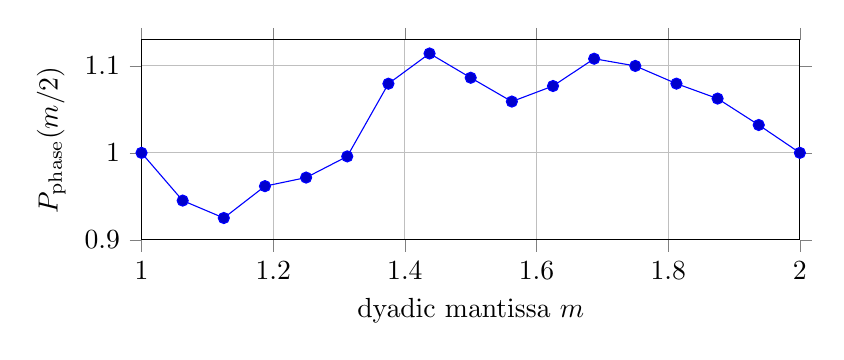
\begin{tikzpicture}
\begin{axis}[
 width=0.82\textwidth,
 height=0.34\textwidth,
 xlabel={dyadic mantissa $m$},
 ylabel={$\ShellPhaseProfile(m/2)$},
 xmin=1,xmax=2,
 ymin=0.90,ymax=1.13,
 grid=major,
 tick align=outside,
]
\addplot+[mark=*] coordinates {
 (1.0000,1.000000000)
 (1.0625,0.945118496)
 (1.1250,0.925107303)
 (1.1875,0.961711083)
 (1.2500,0.971580861)
 (1.3125,0.995925058)
 (1.3750,1.079490550)
 (1.4375,1.114228254)
 (1.5000,1.086316716)
 (1.5625,1.058951765)
 (1.6250,1.076832568)
 (1.6875,1.108201849)
 (1.7500,1.099910476)
 (1.8125,1.079553278)
 (1.8750,1.062385735)
 (1.9375,1.032028829)
 (2.0000,1.000000000)
};
\end{axis}
\end{tikzpicture}
\end{center}

\begin{remark}
A slowly varying correction, including every power of $\log x$, cannot remove this phase.
For a slowly varying $L$, the ratio $L(2^ny)/L(2^n)$ tends uniformly to one for
$y\in[1/2,1]$, so the profile \eqref{eq:phase-limit} survives.  An exact all-phase
normalizer would have to encode the singular conformal distribution, not merely add a
smooth logarithmic factor.
\end{remark}


\subsection{How far the unrestricted Cesaro obstruction extends}
\label{subsec:stabilizing-gauges}

The nonconstant profile in \Cref{thm:phase-limit} is not an artifact of having omitted a
power of $\log x$.  It survives every gauge whose relative shape settles down inside
successive dyadic shells.

\begin{theorem}[Impossibility in the stabilizing class]
\label{thm:stabilizing-impossibility}
Let $g:(X_0,\infty)\to(0,\infty)$ be a gauge.  Suppose there are constants $c_k>0$ and a
continuous $u:[0,1]\to(0,\infty)$ such that
\begin{equation}
 \frac{g(2^k(1+z))}{c_kE_{\kappa_1}(2^k(1+z))}
 \longrightarrow u(z)
 \quad\text{uniformly for }0\le z\le1.
 \label{eq:stabilizing-shape}
\end{equation}
Then the unrestricted limit
\begin{equation}
 \frac1{t-X_0}\int_{X_0}^t\frac{|\FourierTwoPi{\RvachevUp}(x)|}{g(x)}\Differential x\longrightarrow1
 \label{eq:Q2-final}
\end{equation}
cannot hold.
\end{theorem}

\begin{proof}
Assume \eqref{eq:Q2-final}.  If $\CesaroNumerator(t)$ denotes the numerator integral,
then for every fixed
$0\le z_1<z_2\le1$,
\begin{equation}
 \frac{\CesaroNumerator(2^k(1+z_2))-\CesaroNumerator(2^k(1+z_1))}{2^k}
 \longrightarrow z_2-z_1.
 \label{eq:partial-shell-linearity}
\end{equation}
The exact factorization in the coordinates $x=2^k(1+z)$ gives
\[
 \frac{|\FourierTwoPi{\RvachevUp}(2^k(1+z))|}{E_{\kappa_1}(2^k(1+z))}
 =\rho_1^{-(k+1)}W(z)\prod_{j=0}^{k}|\sin(\pi2^jz)|,
\]
where
$W(z)\DefinitionEquals{}W_{\kappa_1}((1+z)/2)=f_1(z)$ is continuous and positive on $[0,1)$.
Combining this identity with
\eqref{eq:stabilizing-shape} and the Ruelle--Perron--Frobenius limit shows that every
subsequential shell limit in \eqref{eq:partial-shell-linearity} is a constant multiple of
\[
 \nu_1\!\left(\frac{W}{u}\IndicatorOf{[z_1,z_2]}\right),
\]
where $\nu_1$ is the eigenmeasure of $\mathcal L_1^*$.  The full-shell case forces the
multiplicative constant to be finite and nonzero.  Equation
\eqref{eq:partial-shell-linearity} would therefore make the measure
$(W/u)\nu_1$ proportional to Lebesgue measure.  Since $W/u$ is continuous and positive on
$[0,1)$ and $\nu_1$ has no endpoint atoms, this would imply $\nu_1\ll\LebesgueMeasure$.

That is impossible.  If $\Differential\nu_1=r\Differential x$ had a nonzero absolutely continuous part, the
eigenmeasure equation would give
\begin{equation}
 |\sin(\pi z)|r(Tz)=\rho_1r(z)
 \quad\text{a.e.}
 \label{eq:conformal-density-final}
\end{equation}
On the positive support of $r$, iteration and Birkhoff's theorem yield
\[
 r(T^nz)=r(z)\frac{\rho_1^n}
 {\prod_{j=0}^{n-1}|\sin(\pi T^jz)|}
 =r(z)\exp\bigl(n(\log(2\rho_1)+\LittleO(1))\bigr).
\]
Here $2\rho_1>1$; for example, Cauchy--Schwarz together with the exact $L^2$ identity and
the Gelfond upper bound gives $\rho_1\ge1/\sqrt3>1/2$, consistently with the rigorous
bracket in \Cref{prop:rho1-rigorous-bound}.  On the other hand, invariance of
Lebesgue measure, Markov's inequality, and Borel--Cantelli imply
$r(T^nz)\le\EulerE^{\varepsilon n}$ eventually for a.e. $z$, for every $\varepsilon>0$.
Choosing $\varepsilon<\log(2\rho_1)$ is a contradiction.  Thus $\nu_1$ is singular and
\eqref{eq:Q2-final} cannot hold.
\end{proof}

The hypothesis covers all gauges of the form
$E_{\kappa_1}(x)L(x)p(\{\log_2x\})$, where $L$ is regularly varying (slow variation is the
most relevant case) and $p$ is positive, continuous, and periodic.  It also covers the
usual log-exp-algebraic or Hardy-field candidates of the correct rough size whenever their
relative logarithmic derivative has a finite limit, because the mean-value theorem then
gives a uniform limiting shell shape.  It does not, by itself, rule out a deliberately
scale-dependent analytic gauge whose within-shell shape keeps changing and attempts to
follow finer and finer dyadic cylinders.  The next theorem removes the assumption that a
limiting shell shape exists.

In shell coordinates put
\begin{equation}
 D_k(z)\DefinitionEquals\frac{\AbsoluteValue{\FourierTwoPi{\RvachevUp}(2^k(1+z))}}{g_1(2^k(1+z))},
 \qquad \Differential\mu_k(z)\DefinitionEquals{}D_k(z)\Differential z,
 \qquad 0\le z\le1.
 \label{eq:shell-finite-measures}
\end{equation}
The RPF limit used in \Cref{thm:phase-limit} says that
$\mu_k\Rightarrow\mu$, $\mu_k([0,1])\to1$, where $\mu$ is an atomless,
full-support singular probability measure.  Full support follows because every open interval
contains a dyadic cylinder and the positive interior transfer weights propagate positive
eigenmeasure mass into every cylinder.

\begin{theorem}[Bounded-distortion obstruction]
\label{thm:bounded-distortion}
Let $X_0>0$ and let $g:[X_0,\infty)\to(0,\infty)$ be measurable.  Suppose there are
constants $0<m<M<\infty$ and numbers $c_k>0$ such that, for every large $k$ and every
$z\in[0,1]$,
\begin{equation}
 m\le
 \frac{g(2^k(1+z))}{c_kg_1(2^k(1+z))}
 \le M.
 \label{eq:bounded-distortion}
\end{equation}
Then $g$ cannot satisfy the unrestricted limit \eqref{eq:Q2-final}.
\end{theorem}

\begin{proof}
Put $a_k\DefinitionEquals\mu_k([0,1])$ and $\bar\mu_k\DefinitionEquals{}a_k^{-1}\mu_k$.  Then
$a_k\to1$ and $\bar\mu_k\Rightarrow\mu$.  After the irrelevant scalar $c_k$ is cancelled,
the probability measure induced on the $k$th shell has the form
\[
 \Differential\eta_k(z)=
 \frac{q_k(z)\Differential\mu_k(z)}{\int_0^1q_k\Differential\mu_k},
 \qquad M^{-1}\le q_k\le m^{-1}.
\]
Since $\int q_k\Differential\mu_k\ge a_k/M$, we have the correctly normalized domination
$\eta_k\le(M/m)\bar\mu_k$: for every continuous $\varphi\ge0$,
\[
 \int\varphi\Differential\eta_k\le\frac{M}{m}\int\varphi\Differential\bar\mu_k.
\]
Any weak limit $\eta$ is therefore dominated by $(M/m)\mu$ and is singular.  But
\eqref{eq:Q2-final}, evaluated at $2^k$ and $2^k(1+z)$ and subtracted, forces the partial
shell masses to converge uniformly to $z$; hence $\eta_k$ must converge to Lebesgue
measure.  This contradiction proves the theorem.
\end{proof}

\begin{corollary}[Necessary shell microstructure]
\label{cor:necessary-microstructure}
Every gauge satisfying the unrestricted ordinary Cesaro limit must have unbounded
within-shell distortion relative to $g_1$, even after an arbitrary scalar renormalization
on each shell.
\end{corollary}

\begin{proof}
Otherwise some $m,M$ and shell scalars $c_k$ would satisfy
\eqref{eq:bounded-distortion}, contradicting \Cref{thm:bounded-distortion}.
\end{proof}

The word ``elementary'' must not be substituted for the hypotheses above.  For instance,
if $2c\varepsilon<1/a$, then
\[
 g_{\varepsilon,c}(x)
 \DefinitionEquals{}g_1(x)\exp\!\bigl(\varepsilon\sin(c(\log x)^2)\bigr)
\]
is elementary, positive, real-analytic, and eventually decreasing, but its shell shape need
not stabilize.  It still fails by \Cref{thm:bounded-distortion}, because the multiplier is
uniformly bounded above and below.  Thus no implication ``Hardy-field, hence elementary''
is valid here.

\section{A shell-adaptive analytic gauge with the exact unrestricted limit}
\label{sec:adaptive-gauge}

The bounded-distortion theorem also tells us how an exact gauge must look: it must resolve
progressively finer portions of the singular shell measure.  The deterministic baseline is
so steep that such a slowly increasing amount of microstructure can be inserted while the
total gauge remains decreasing.  This section gives the construction in full.

\subsection{Smooth asymptotic flattening}

\begin{lemma}[Smooth flattening of weakly convergent measures]
\label{lem:flattening}
Let $\mu_k$ be finite positive Borel measures on $[0,1]$ converging weakly to an atomless,
fully supported probability measure $\mu$, with $\mu_k([0,1])\to1$.  There are functions
$r_k\in C^\infty([0,1])$, $r_k>0$, such that
\begin{enumerate}
\item $r_k\equiv1$ in neighborhoods of $0$ and $1$;
\item
\begin{equation}
 \sup_{0\le z\le1}
 \left|\int_0^zr_k\Differential\mu_k-z\right|\longrightarrow0;
 \label{eq:flattening-cdf}
\end{equation}
\item
\begin{equation}
 \Norm{\log r_k}_\infty=\LittleO(k),
 \qquad
 \Norm{(\log r_k)'}_\infty=\LittleO(k).
 \label{eq:flattening-slopes}
\end{equation}
\end{enumerate}
\end{lemma}

\begin{proof}
Choose finite partitions
$0=x_{j,0}<x_{j,1}<\cdots<x_{j,N_j}=1$ whose meshes
$\varepsilon_j$ tend to zero.  Because $\mu$ is atomless, the boundary points may be taken
to be continuity points; because it has full support, every cell
$I_{j,i}=[x_{j,i-1},x_{j,i}]$ has positive mass.  For fixed $j$, weak convergence gives
$\mu_k(I_{j,i})\to\mu(I_{j,i})$ simultaneously over the finite partition.  Define the
cell equalizer
\[
 c_{k,j,i}\DefinitionEquals\frac{|I_{j,i}|}{\mu_k(I_{j,i})}.
\]

For fixed $j$, the finitely many ratios $c_{k,j,i}$ converge to positive finite limits.
Choose $B_j$ large enough that $|\log c_{k,j,i}|\le B_j/2$ for every cell and all large
$k$.  Now let $U_j$ be a finite union of sufficiently small intervals around all partition
boundaries, including $0$ and $1$, such that $\mu(\partial U_j)=0$ and
$\mu(U_j)+|U_j|$ is smaller than $\varepsilon_je^{-B_j}/20$.  Weak convergence then gives
$\mu_k(U_j)\to\mu(U_j)$.  Set $\ell_{k,j}=\log c_{k,j,i}$ on each cell outside $U_j$, join
these finitely many constants smoothly inside $U_j$, and arrange $\ell_{k,j}=0$ near the
endpoints.  The interpolation can be kept between its neighboring values and chosen with
bounds
\[
 \Norm{\ell_{k,j}}_\infty\le B_j,
 \qquad
 \Norm{\ell_{k,j}'}_\infty\le C_j.
\]
Put $r_{k,j}=\exp\ell_{k,j}$.  On a cell $I=I_{j,i}$ the definition
$c_{k,j,i}\mu_k(I)=|I|$ gives the exact error identity
\[
 \int_I r_{k,j}\Differential\mu_k-|I|
 =\int_{I\cap U_j}(r_{k,j}-c_{k,j,i})\Differential\mu_k.
\]
Thus the total error over any union of complete cells is at most
$2e^{B_j}\mu_k(U_j)$.  A cumulative interval $[0,z]$ has, in addition, at most one
partially traversed cell.  Its portion outside $U_j$ has weighted mass at most the full
cell length, hence at most the mesh, while its portion inside $U_j$ is bounded by
$e^{B_j}\mu_k(U_j)$; the omitted Lebesgue length is bounded in the same way by the mesh
and $|U_j|$.  Our choice of $U_j$, followed by large $k$, therefore gives (after harmlessly
rescaling the sequence $\varepsilon_j$)
\[
 \sup_z\left|\int_0^zr_{k,j}\Differential\mu_k-z\right|\le3\varepsilon_j.
\]

Choose increasing integers $K_j$ so that these conclusions hold for $k\ge K_j$ and
additionally
\[
 B_j/K_j\le\varepsilon_j,
 \qquad C_j/K_j\le\varepsilon_j.
\]
For $K_j\le k<K_{j+1}$ set $r_k=r_{k,j}$.  Then $j=j(k)\to\infty$, so the cumulative
error tends to zero and both estimates in \eqref{eq:flattening-slopes} hold.  The endpoint
condition was built into every interpolation.
\end{proof}

\subsection{The smooth exact gauge}

Apply \Cref{lem:flattening} to the measures in
\eqref{eq:shell-finite-measures}.  Define a multiplier $R$ on every sufficiently large
shell by
\begin{equation}
 R(2^k(1+z))\DefinitionEquals{}r_k(z),
 \qquad 0\le z\le1.
 \label{eq:R-global}
\end{equation}
Because $r_k=1$ in neighborhoods of both endpoints, adjacent pieces agree with all
derivatives near every power of two; hence $R$ is globally smooth on a half-line.  Put
\begin{equation}
 h_0(x)\DefinitionEquals\frac1{g_1(x)},
 \qquad h(x)\DefinitionEquals{}h_0(x)R(x),
 \qquad g_\infty(x)\DefinitionEquals\frac1{h(x)}.
 \label{eq:smooth-adaptive-gauge}
\end{equation}
In shell coordinates,
\begin{equation}
 \frac{\partial}{\partial z}\log h_0(2^k(1+z))
 =\frac{k+\kappa_1+a^{-1}\log(1+z)}{1+z}\ge\frac{k}{3}
 \label{eq:baseline-slope}
\end{equation}
for all large $k$, uniformly in $z$.  Equation \eqref{eq:flattening-slopes} therefore makes
$h$ eventually strictly increasing and $g_\infty$ eventually strictly decreasing.  It also
gives
\begin{equation}
 \log g_\infty(x)=\log g_1(x)+\LittleO(\log x).
 \label{eq:smooth-rough-scale}
\end{equation}

\begin{proposition}[Smooth exact arithmetic gauge]
\label{prop:smooth-adaptive}
For every fixed sufficiently large $X_0$,
\begin{equation}
 \frac1{t-X_0}\int_{X_0}^{t}
 \frac{\AbsoluteValue{\FourierTwoPi{\RvachevUp}(x)}}{g_\infty(x)}\Differential x\longrightarrow1.
 \label{eq:smooth-exact-limit}
\end{equation}
\end{proposition}

\begin{proof}
Let
\[
 C_k(z)\DefinitionEquals\int_0^zD_k(u)r_k(u)\Differential u.
\]
By \Cref{lem:flattening}, $\sup_z|C_k(z)-z|\to0$.  If
$t=2^K(1+z)$, complete and partial shells give, up to one fixed initial contribution,
\[
 \int_{X_0}^{t}\frac{\AbsoluteValue{\FourierTwoPi{\RvachevUp}(x)}}{g_\infty(x)}\Differential x
 =\sum_{k<K}2^kC_k(1)+2^KC_K(z).
\]
Replacing $C_k(1)$ by $1$ and $C_K(z)$ by $z$ costs $\LittleO(2^K)$: indeed
$\sum_{k<K}2^k\epsilon_k=\LittleO(2^K)$ whenever $\epsilon_k\to0$.  The main term is
$\sum_{k<K}2^k+2^Kz=t+\BigO(1)$, after absorbing the fixed choice of initial shell.
Division by $t-X_0$ proves \eqref{eq:smooth-exact-limit}.
\end{proof}

\subsection{Real-analytic upgrade by Carleman--Hoischen approximation}

We use the following precise classical input: if $f\in C^1(\RealNumbers)$ and
$\epsilon:\RealNumbers\to(0,\infty)$ is continuous, there is an entire function $g$, real on the
real axis, such that
\begin{equation}
 \AbsoluteValue{g(x)-f(x)}<\epsilon(x),
 \qquad \AbsoluteValue{g'(x)-f'(x)}<\epsilon(x)
 \quad(x\in\RealNumbers).
 \label{eq:Hoischen}
\end{equation}
This is Hoischen's derivative form of Carleman approximation; we use the formulation of
Gauthier and Kienzle \cite{gauthier-kienzle}.

Extend $h$ in \eqref{eq:smooth-adaptive-gauge} to a positive $C^1$ function on $\RealNumbers$
such that $h'(x)>0$ for every $x$.  This is possible because
\eqref{eq:baseline-slope} makes $h'$ positive on the retained tail; before a joining point,
a positive exponential chosen to match its value and first derivative supplies a $C^1$
extension.  Choose a continuous $\delta(x)>0$ with $\delta(x)\to0$ as $x\to+\infty$,
then choose a continuous positive tolerance $\epsilon$ satisfying
\begin{equation}
 \epsilon(x)<\frac12\min\{h(x),h'(x),\delta(x)h(x)\}.
 \label{eq:Hoischen-error}
\end{equation}
The real entire approximant $\widetilde h$ is positive and strictly increasing on $\RealNumbers$,
and $\widetilde h/h\to1$ at $+\infty$.  Define
\begin{equation}
 g_{\mathrm{ad}}(x)\DefinitionEquals\frac1{\widetilde h(x)},
 \qquad x>0.
 \label{eq:g-adaptive}
\end{equation}

\begin{theorem}[Literal analytic solution of the original Cesaro problem]
\label{thm:analytic-adaptive}
The gauge $g_{\mathrm{ad}}$ is positive, real-analytic, and strictly decreasing.  For every
fixed $t_0>0$ it satisfies
\begin{equation}
 \frac1{t-t_0}\int_{t_0}^{t}
 \frac{\AbsoluteValue{\FourierTwoPi{\RvachevUp}(x)}}{g_{\mathrm{ad}}(x)}\Differential x\longrightarrow1,
 \label{eq:adaptive-exact-limit}
\end{equation}
and
\begin{equation}
 \log g_{\mathrm{ad}}(x)
 =-\frac{(\log x)^2}{2\log2}-\kappa_1\log x+\LittleO(\log x).
 \label{eq:adaptive-rough-scale}
\end{equation}
\end{theorem}

\begin{proof}
The regularity and monotonicity follow from the construction.  The rough scale follows from
$\widetilde h/h\to1$, \eqref{eq:smooth-rough-scale}, and the definition of $g_1$.
For the integral, fix $\varepsilon>0$ and choose $X$ so that
$|\widetilde h/h-1|<\varepsilon$ for $x\ge X$.  Since $1/g_{\mathrm{ad}}=\widetilde h$
and $1/g_\infty=h$,
\[
 \left|\int_X^t\AbsoluteValue{\FourierTwoPi{\RvachevUp}(x)}(\widetilde h(x)-h(x))\Differential x\right|
 \le\varepsilon\int_X^t\AbsoluteValue{\FourierTwoPi{\RvachevUp}(x)}h(x)\Differential x
 =\varepsilon(t+\LittleO(t))
\]
by \Cref{prop:smooth-adaptive}.  The initial interval contributes $\BigO(1)$.  Divide by
$t$ and then let $\varepsilon\downarrow0$.
\end{proof}

\begin{remark}[Why there is no contradiction]
The natural profile is driven by the distribution function of an atomless singular measure,
but the profile itself also contains the ordinary factor $1/y$ and is not itself a singular
distribution function.  The multiplier $r_k$ corrects only finitely many cells at
level $k$, while the number of cells tends to infinity.  Its logarithm and logarithmic
slope are $\LittleO(k)$, so the gauge remains decreasing, yet its normalized shell shape never
converges and its distortion becomes unbounded.  Thus neither
\Cref{thm:stabilizing-impossibility} nor \Cref{thm:bounded-distortion} applies.
\end{remark}

\begin{remark}[Higher derivatives]
The natural gauge $g_1$ has alternating derivative signs eventually for each fixed order.
The adaptive construction above guarantees positivity and strict decrease, but not one
common tail on which every higher derivative has a prescribed sign.  Preserving any chosen
finite number of signs should be approachable by a higher-order Carleman--Hoischen theorem
and a slower diagonal selection, but the required derivative error budget is not proved
here.  We record that strengthening as a frontier rather than as a theorem.
\end{remark}

\begin{boxedremark}
Lean currently formalizes the shell-linearity reduction, finite-partition measure
equalization, and diagonal-selection core in \lean{ShellLinearity},
\lean{MeasureEqualization}, and \lean{DiagonalSelection}.  The RPF convergence, smooth
gluing, and Carleman--Hoischen approximation remain explicitly identified analytic inputs.
\end{boxedremark}

\section{The multiplicatively natural logarithmic mean}
\label{sec:logarithmic-mean}

The endpoint obstruction disappears if additive Cesaro averaging is replaced by logarithmic
averaging.  Each dyadic shell then has equal weight, and the final incomplete shell becomes
negligible.

\begin{theorem}[Unrestricted logarithmic mean]
\label{thm:logarithmic-mean}
There is a constant $A_1^{\log}>0$ such that, for every fixed $t_0>1$,
\begin{equation}
 \frac1{\log(t/t_0)}\int_{t_0}^t
 \frac{|\FourierTwoPi{\RvachevUp}(x)|}{E_{\kappa_1}(x)}\frac{\Differential x}{x}
 \longrightarrow A_1^{\log}
 \qquad(t\to\infty)
 \label{eq:logarithmic-mean}
\end{equation}
without any restriction on the endpoint.  In the normalization of
\Cref{prop:RPF}, if
$f_1(x)=W_{\kappa_1}((x+1)/2)$, then
\begin{equation}
 B_1\DefinitionEquals\left(\int_0^1h_1(x)\Differential x\right)
 \nu_1\!\left(\frac{f_1}{1+\cdot}\right),
 \qquad
 A_1^{\log}\DefinitionEquals\frac{B_1}{\log2}.
 \label{eq:A1log}
\end{equation}
Numerically,
\begin{equation}
 A_1^{\log}=0.09386063575678126354\ldots .
 \label{eq:A1log-numeric}
\end{equation}
\end{theorem}

\begin{proof}
Let
\[
 \beta_n=\int_{2^{n-1}}^{2^n}
 \frac{|\FourierTwoPi{\RvachevUp}(x)|}{E_{\kappa_1}(x)}\frac{\Differential x}{x}.
\]
The master factorization and $x=2^ny$, followed by $z=2y-1$, give
\[
 \beta_n=\rho_1^{-n}\int_0^1
 \frac{f_1(z)}{1+z}\prod_{j=0}^{n-1}|\sin(\pi T^jz)|\Differential z.
\]
The spectral limit in \Cref{prop:RPF} yields $\beta_n\to\beta_\infty$, where
$\beta_\infty=(\int h_1)\nu_1(f_1/(1+\cdot))$.  If
$2^N\le t<2^{N+1}$, the logarithmic integral equals
$\sum_{n<N}\beta_n+\BigO(1)$, while $\log(t/t_0)=N\log2+\BigO(1)$.  Ordinary Cesaro convergence of
the sequence $(\beta_n)$ proves \eqref{eq:logarithmic-mean} and
\eqref{eq:A1log}.
\end{proof}

\section{The sharp uniform envelope}
\label{sec:uniform}

The $L^\infty$ numerator rate can be proved by a sharp elementary inequality.  Put
\begin{equation}
 \lambda\DefinitionEquals\frac{\sqrt3}{2}.
 \label{eq:lambda}
\end{equation}

\begin{lemma}[Sharp two-step logarithmic inequality]
\label{lem:sharp-sine-inequality}
For every $x\in\RealNumbers$,
\begin{equation}
 \frac23\log s(x)+\frac13\log s(Tx)\le\log\lambda,
 \label{eq:weighted-log-inequality}
\end{equation}
with the usual interpretation at zeros.  Equality holds precisely when
$x\equiv1/3$ or $2/3\pmod1$.
\end{lemma}

\begin{proof}
Cubing the desired inequality gives
\[
 s(x)^2s(Tx)\le\lambda^3.
\]
With $\theta=\pi x$ and $u=\sin^2\theta$,
\[
 s(x)^2s(Tx)=2\AbsoluteValue{\sin^3\theta\cos\theta},
\]
whose square is $4u^3(1-u)$.  The maximum of $u^3(1-u)$ on $[0,1]$ is $27/256$, attained
at $u=3/4$.  Therefore the maximum of the original expression is
$3\sqrt3/8=\lambda^3$, with equality at $x\equiv1/3,2/3$.
\end{proof}

\begin{proposition}[Uniform lacunary-product bound]
\label{prop:Bn-uniform}
For every $n\ge1$,
\begin{equation}
 \lambda^n\le\sup_{x\in[0,1]}
 \prod_{j=0}^{n-1}s(T^jx)\le\lambda^{n-1}.
 \label{eq:Bn-uniform}
\end{equation}
Consequently
\begin{equation}
 \lim_{n\to\infty}\Norm{\prod_{j=0}^{n-1}s\circ T^j}_{\infty}^{1/n}
 =\lambda=\frac{\sqrt3}{2}.
 \label{eq:Gelfond-rate}
\end{equation}
\end{proposition}

\begin{proof}
At $x=1/3$ the orbit alternates between $1/3$ and $2/3$, and every factor equals
$\lambda$, proving the lower bound.  For $n=1$ the upper bound is
$\sup s=1=\lambda^0$.  Assume henceforth that $n\ge2$.  For the upper bound, sum
\eqref{eq:weighted-log-inequality} for $x,Tx,\dots,T^{n-2}x$.  If
$\phi=\log s$, the result is
\[
 3\sum_{j=0}^{n-2}\phi(T^jx)-\phi(x)+\phi(T^{n-1}x)
 \le3(n-1)\log\lambda.
\]
After adding the final factor,
\[
 \sum_{j=0}^{n-1}\phi(T^jx)
 \le(n-1)\log\lambda+\frac13\phi(x)+\frac23\phi(T^{n-1}x)
 \le(n-1)\log\lambda,
\]
because $\phi\le0$.  Exponentiation gives the upper bound.
\end{proof}

This is the classical Gelfond exponent for the Thue--Morse polynomial: by
\eqref{eq:TM-modulus}, the unnormalized polynomial grows like $3^{n/2}$ in supremum norm.
The ergodic-optimization formulation and its generalizations are developed in
\cite{fan-schmeling-shen}.

\begin{theorem}[Sharp global upper envelope]
\label{thm:uniform-envelope}
Define
\begin{equation}
 \boxed{\displaystyle
 \kappa_\infty
 \DefinitionEquals\frac{\log\pi+a/2-\log(\sqrt3/2)}{a}
 =\frac32+\frac{\log(\pi/\sqrt3)}{\log2}
 =2.3590148791117407073\ldots .}
 \label{eq:kappa-infty}
\end{equation}
Then there is a constant $C<\infty$ such that
\begin{equation}
 \AbsoluteValue{\FourierTwoPi{\RvachevUp}(x)}\le C E_{\kappa_\infty}(x),
 \qquad x\ge1.
 \label{eq:uniform-envelope}
\end{equation}
This exponent is sharp.  In fact, for every $n\ge0$,
\begin{equation}
 \AbsoluteValue{\FourierTwoPi{\RvachevUp}(2^n\cdot2/3)}
 =C_*E_{\kappa_\infty}(2^n\cdot2/3),
 \label{eq:exact-peak-ray}
\end{equation}
where
\begin{equation}
 C_*=W_{\kappa_\infty}(2/3)>0.
 \label{eq:Cstar}
\end{equation}
Numerically, $C_*=0.139129774734829\ldots$; the exact content is the preceding value of
$W_{\kappa_\infty}$, not a certified decimal enclosure.
\end{theorem}

\begin{proof}
In \eqref{eq:master-normalization}, the definition of $\kappa_\infty$ makes
\[
 \exp(n(\kappa_\infty a-\log\pi-a/2))=\lambda^{-n}.
\]
After the substitution $x=Ty$, the product is of the form bounded in
\eqref{eq:Bn-uniform}; therefore
\[
 \frac{\AbsoluteValue{\FourierTwoPi{\RvachevUp}(2^ny)}}{E_{\kappa_\infty}(2^ny)}
 \le\lambda^{-1}\max_{1/2\le y\le1}W_{\kappa_\infty}(y).
\]
This proves the uniform upper bound.  At $y=2/3$, the orbit alternates between $2/3$ and
$1/3$, so $B_n(2/3)=\lambda^n$ exactly.  Equation
\eqref{eq:master-normalization} then reduces to \eqref{eq:exact-peak-ray}.
\end{proof}

\begin{corollary}[Universal logarithmic order]
\label{cor:universal-log-order}
With the convention $\log0=-\infty$,
\begin{equation}
 \limsup_{x\to\infty}\frac{\log|\FourierTwoPi{\RvachevUp}(x)|}{(\log x)^2}
 =-\frac1{2\log2},
 \qquad
 \liminf_{x\to\infty}\frac{\log|\FourierTwoPi{\RvachevUp}(x)|}{(\log x)^2}=-\infty.
 \label{eq:universal-log-order}
\end{equation}
Equivalently, the coefficient $1/(2\log2)$ is the sharp global log-square order, but no
positive two-sided pointwise equivalent exists.
\end{corollary}

\begin{proof}
The upper bound in the limsup follows from \eqref{eq:uniform-envelope}; the exact period-two
ray \eqref{eq:exact-peak-ray} gives the reverse inequality.  The liminf is $-\infty$ because
$\FourierTwoPi{\RvachevUp}$ vanishes at every positive integer (and also because one may approach those zeros
arbitrarily closely).
\end{proof}

\begin{corollary}[Sharp smoothness class]
\label{cor:superpoly-subexp}
For every $M>0$, $\FourierTwoPi{\RvachevUp}(x)=\BigO(x^{-M})$ as $x\to\infty$.  On the other hand, for every
$c>0$, $\EulerE^{cx}\AbsoluteValue{\FourierTwoPi{\RvachevUp}(x)}$ is unbounded.  Thus the transform decays faster than every
power but not at any fixed exponential rate.
\end{corollary}

\begin{proof}
The first statement follows from \eqref{eq:uniform-envelope}, because the negative
quadratic in $\log x$ dominates $-M\log x$.  The exact peak ray
\eqref{eq:exact-peak-ray} decays only like $\exp(-\BigO((\log x)^2))$, which is much larger
than $\EulerE^{-cx}$ along that subsequence.
\end{proof}


\section{The raw dyadic-annulus maximum and its Lambert boundary layer}
\label{sec:annular-maxima}

The sharp pointwise envelope of \Cref{thm:uniform-envelope} is evaluated at the actual
argument $x$.  A different question is to compare every value in the shell
$[2^k,2^{k+1}]$ with the envelope at its \emph{left endpoint}.  The maximizer then moves
toward that endpoint and pays a second, slower log-normal cost.  This is the main result of
Wave 1, Document 2 \cite{wave1-doc2}; we reproduce the proof because it is the most delicate
asymptotic in the corpus.

Put
\begin{equation}
 \mathfrak M_k\DefinitionEquals\max_{2^k\le x\le2^{k+1}}|\FourierTwoPi{\RvachevUp}(x)|,
 \qquad n\DefinitionEquals{}k+1,
 \qquad \beta\DefinitionEquals\log\frac{\sqrt3}{2}<0.
 \label{eq:annular-M}
\end{equation}
Also define the tail factor
\[
 \mathcal H(y)\DefinitionEquals\prod_{m=1}^{\infty}\left|\SincRad\!\left(\frac{\pi y}{2^m}\right)\right|,
 \qquad y\in\RealNumbers.
\]
Thus $\mathcal H(y)=|\FourierTwoPi{\RvachevUp}(y/2)|$ globally.  In particular it is continuous and bounded;
on compact sets avoiding the nonzero even integers it is bounded away from zero.

\subsection{Exact reduction and transition coordinates}

Writing $x=2^k(1+\theta)$, $0\le\theta\le1$, gives
\begin{equation}
 |\FourierTwoPi{\RvachevUp}(2^k(1+\theta))|
 =\frac{2^{-k(k+1)/2}}{\pi^n}
 \mathcal H(1+\theta)(1+\theta)^{-n}Q_n(\theta),
 \label{eq:annular-exact-final}
\end{equation}
where
\[
 Q_n(\theta)=\prod_{j=0}^{n-1}|\sin(\pi2^j\theta)|.
\]
Hence
\begin{equation}
 \mathfrak M_k=\pi^{-n}2^{-k(k+1)/2}A_n,
 \quad
 A_n\DefinitionEquals\sup_{0\le\theta\le1}
 \mathcal H(1+\theta)(1+\theta)^{-n}Q_n(\theta).
 \label{eq:An-final}
\end{equation}
The weight $(1+\theta)^{-n}$ pushes the maximum toward $0$, where $Q_n$ vanishes.
For $0<\theta\le1/2$, write uniquely up to endpoints
\begin{equation}
 \theta=2^{-r}s,
 \qquad r\in\NaturalNumbers,\quad s\in I\DefinitionEquals[1/4,1/2].
 \label{eq:transition-final}
\end{equation}
If $r<n$, then
\begin{equation}
 Q_n(2^{-r}s)=R_r(s)Q_{n-r}(s),
 \quad
 R_r(s)=\prod_{h=1}^{r}\sin\!\left(\frac{\pi s}{2^h}\right).
 \label{eq:transition-product-final}
\end{equation}
Uniformly for $s\in I$,
\begin{equation}
 \log R_r(s)
 =-\frac a2r^2+r\left(\log(\pi s)-\frac a2\right)+\BigO(1).
 \label{eq:small-block-final}
\end{equation}
The remaining tail satisfies $Q_m(s)\le C\EulerE^{m\beta}$ by
\Cref{prop:Bn-uniform}.

For a matching lower bound one needs near-maximizing tails at essentially arbitrary $s$.

\begin{lemma}[Dense preimages of the maximizing cycle]
\label{lem:dense-preimages-final}
There is $C>0$ such that for every $s_0\in I$ and $q\ge1$ one can choose $s_q\in I$ with
\begin{equation}
 |s_q-s_0|\le2^{-q},
 \qquad T^qs_q\in\{1/3,2/3\},
 \label{eq:preimage-close-final}
\end{equation}
and, for every $m\ge q$,
\begin{equation}
 Q_m(s_q)\ge\exp(m\beta-Cq^2).
 \label{eq:preimage-lower-final}
\end{equation}
\end{lemma}

\begin{proof}
The $q$-fold preimages $(j+1/3)/2^q$ have spacing $2^{-q}$; together with the preimages of
$2/3$ they approximate every point of $I$ as in \eqref{eq:preimage-close-final}.  Before
time $q$, every orbit point is a nonintegral rational with reduced denominator at most
$3\cdot2^{q-j}$.  Therefore
\[
 |\sin(\pi T^js_q)|\ge2\MetricDistance(T^js_q,\IntegerNumbers)
 \ge\frac{2}{3\cdot2^{q-j}}.
\]
The first $q$ factors lose at most $\exp(\BigO(q^2))$.  Thereafter the orbit alternates between
$1/3$ and $2/3$, and every factor equals $\sqrt3/2=\EulerE^\beta$.
\end{proof}

Define the finite-dimensional objective
\begin{equation}
 \DecayOptimizationObjective{n}(r,s)
 =-\frac a2r^2+r\left(\log(\pi s)-\frac a2-\beta\right)
 -n\log(1+s2^{-r}).
 \label{eq:Fn-final}
\end{equation}

\begin{lemma}[Reduction to the boundary-layer objective]
\label{lem:An-reduction-final}
As $n\to\infty$,
\begin{equation}
 \log A_n=n\beta+
 \sup_{\substack{r\in\NaturalNumbers\\s\in I}}\DecayOptimizationObjective{n}(r,s)
 +\BigO((\log\log n)^2).
 \label{eq:An-reduction-final}
\end{equation}
\end{lemma}

\begin{proof}
First take $0<\theta\le1/2$, write $\theta=2^{-r}s$, and suppose $r<n$.
Equations \eqref{eq:transition-product-final}--\eqref{eq:small-block-final} and the uniform
Gelfond bound give, uniformly in $r,s$,
\begin{equation}
 \log\!\left(\mathcal H(1+\theta)(1+\theta)^{-n}Q_n(\theta)\right)
 \le n\beta+\DecayOptimizationObjective{n}(r,s)+C.
 \label{eq:An-phase-upper}
\end{equation}
Here $\mathcal H$ is bounded on $[1,2]$.  If $\theta\ge1/2$, the left side is at most
$-n\log(3/2)+\BigO(1)$.  If $r\ge n$, the elementary bounds
$|\sin u|\le|u|$ give
\[
 \log Q_n(2^{-r}s)
 \le n\log(\pi s)+a\frac{n(n-1)}2-anr,
\]
so this range is $-\Omega(n^2)$.  Both are exponentially inferior to the admissible trial
$r=\Floor{\log_2n}$, $s=1/3$, whose tail lies exactly on the maximizing two-cycle and
whose logarithm is $n\beta-\BigO((\log n)^2)$.  This proves that every phase within
$\BigO((\log\log n)^2)$ of the maximum has $r<n$.

The same comparison yields the two uniform localization estimates used below.  Since
$s\in[1/4,1/2]$,
\[
 \DecayOptimizationObjective{n}(r,s)\le-\frac a2r^2+C_1r,
 \qquad
 \log(1+s2^{-r})\ge\frac12s2^{-r}.
\]
Comparison with the trial value first gives $r=\BigO(\log n)$ and then, after retaining the
last negative term in $\DecayOptimizationObjective{n}$,
\begin{equation}
 ns2^{-r}=\BigO((\log n)^2).
 \label{eq:boundary-localization}
\end{equation}
Thus \eqref{eq:An-phase-upper} gives the desired upper bound by taking the supremum of
$\DecayOptimizationObjective{n}$.

For the reverse inequality choose a localized pair $(r,s)$ within one of the supremum of
$\DecayOptimizationObjective{n}$ and put
$q=\Ceiling{4\log_2\log(n+\EulerE^\EulerE)}$.  For large $n$ we have $n-r\ge q$.
Choose $s_q$ by \Cref{lem:dense-preimages-final}.  In the localized region
\[
 \left|\frac{\partial\DecayOptimizationObjective{n}}{\partial s}\right|
 \le4r+n2^{-r}=\BigO((\log n)^2),
\]
so $|\DecayOptimizationObjective{n}(r,s_q)-\DecayOptimizationObjective{n}(r,s)|=\BigO(1)$.  The dense-preimage lower bound gives
\[
 \log Q_{n-r}(s_q)\ge(n-r)\beta-Cq^2,
\]
while \eqref{eq:small-block-final} supplies the matching prefix and
$\mathcal H(1+2^{-r}s_q)$ is bounded below because its argument tends to $1$.
Consequently the resulting phase has logarithm at least
\[
 n\beta+\sup_{r,s}\DecayOptimizationObjective{n}(r,s)-\BigO(q^2).
\]
Since $q^2=\BigO((\log\log n)^2)$, this completes both sides of
\eqref{eq:An-reduction-final}.
\end{proof}

\subsection{Lambert optimization}

Set
\begin{equation}
 C_0\DefinitionEquals\log\pi-\frac a2-\beta=\log\!\left(\pi\sqrt{\frac23}\right),
 \qquad
 c\DefinitionEquals{}a\EulerE^{-C_0}=\frac a\pi\sqrt{\frac32}.
 \label{eq:annular-c}
\end{equation}
At the localized maximum, \eqref{eq:boundary-localization} implies
\[
 n\left|\log(1+s2^{-r})-s2^{-r}\right|
 =O\!\left(\frac{(\log n)^4}{n}\right)=\LittleO(1).
\]
Put $A=C_0+\log s$ and $z=ar-A$.  Then
\begin{equation}
 -\frac a2r^2+rA-ns2^{-r}
 =-\frac{z^2}{2a}-n\EulerE^{-C_0}\EulerE^{-z}+\frac{A^2}{2a}.
 \label{eq:z-objective}
\end{equation}
As $s$ traverses $[1/4,1/2]$, the interval of possible $A$ has length exactly $a$.
Successive integer values of $r\ge0$ therefore make the corresponding $z$-intervals tile a
half-line.  That half-line contains the maximizer below for all large $n$.  Since
$A^2/(2a)=\BigO(1)$, the supremum is, up to $\BigO(1)$, the real maximum of
\[
 \phi_n(z)=-\frac{z^2}{2a}-n\EulerE^{-C_0}\EulerE^{-z}.
\]
Its critical equation is $z\EulerE^z=cn$, so the maximizer is $w_n=W(cn)$ and
we use the principal real branch of $W$ throughout \cite{corless-lambert}.  Thus
\begin{equation}
 \max\phi_n=-\frac{w_n^2+2w_n}{2a}.
 \label{eq:Lambert-value}
\end{equation}

\begin{theorem}[Sharp dyadic-annulus maximum]
\label{thm:annular-main}
Let $w_k=W(c(k+1))$, with $c$ from \eqref{eq:annular-c}.  Then, as $k\to\infty$,
\begin{equation}
 \boxed{\displaystyle
 \log\mathfrak M_k
 =-\frac a2k(k+1)-(k+1)\log\pi+(k+1)\beta
 -\frac{w_k^2+2w_k}{2a}
 +\BigO((\log\log k)^2).}
 \label{eq:annular-main}
\end{equation}
Equivalently,
\begin{equation}
 \log\mathfrak M_k
 =-\frac a2k^2-a\kappa_\infty k
 -\frac{W(c(k+1))^2+2W(c(k+1))}{2a}
 +\BigO((\log\log k)^2).
 \label{eq:annular-main-compact}
\end{equation}
Any maximizing phase $\theta_k$ satisfies
\begin{equation}
 \theta_k=\frac{W(c(k+1))}{a(k+1)}\EulerE^{\LittleO(1)}.
 \label{eq:annular-location}
\end{equation}
\end{theorem}

\begin{proof}
Combine \eqref{eq:An-final}, \Cref{lem:An-reduction-final}, and
\eqref{eq:Lambert-value}.  The compact form uses
$a\kappa_\infty=a/2+\log\pi-\beta$.

For the location statement, \eqref{eq:An-phase-upper} and the matching lower bound show
that the $z$ associated with any maximizing phase satisfies
$\phi_n(w_n)-\phi_n(z)=\BigO((\log\log n)^2)$.  Writing $z=w_n+u$ and using
$n\EulerE^{-C_0-w_n}=w_n/a$, one has
\[
 \phi_n'(w_n+u)=\frac{w_n(\EulerE^{-u}-1)-u}{a}.
\]
For $u\le0$ this gives a loss at least $w_nu^2/(2a)$; for $0\le u\le1$ it gives the same
bound up to an absolute constant.  A displacement $u\ge1$ already costs a fixed positive
multiple of $w_n$.  Since $w_n\asymp\log n$ while $(\log\log n)^2=\LittleO(w_n)$, every maximizer
therefore satisfies
\[
 z=w_n+O\!\left(\frac{\log\log n}{\sqrt{w_n}}\right)=w_n+\LittleO(1).
\]
Since
$\theta=s2^{-r}=\EulerE^{-C_0-z}$ and
$n\EulerE^{-C_0-w_n}=w_n/a$, this gives \eqref{eq:annular-location}.
\end{proof}

Let $R=2^k$, $L=\log R$, and $d=\pi^{-1}\sqrt{3/2}$.  Since
$c(k+1)=d(L+a)$, \eqref{eq:annular-main-compact} becomes
\begin{equation}
 \log\max_{R\le x\le2R}|\FourierTwoPi{\RvachevUp}(x)|
 =-\frac{L^2}{2a}-\kappa_\infty L
 -\frac{W(d(L+a))^2+2W(d(L+a))}{2a}
 +\BigO((\log\log\log R)^2).
 \label{eq:annular-physical}
\end{equation}
The extra term begins
\begin{equation}
 -\frac{(\log\log R)^2}{2a}
 +\frac{\log\log R\,\log\log\log R}{a}
 +\BigO(\log\log R).
 \label{eq:second-lognormal}
\end{equation}
Thus the annular maximum is smaller than the left-endpoint envelope
$E_{\kappa_\infty}(R)$ by a second log-normal factor, even though the pointwise-envelope
rate is realized exactly up to $C_*$ on the fixed ray $x=2^n(2/3)$.  There is no
contradiction: the
fixed ray is a constant fraction into its shell, whereas the raw annular maximizer migrates
toward the left boundary according to \eqref{eq:annular-location}.

\section{Exceptional extrema near dyadic boundaries}
\label{sec:exceptional-extrema}

The sharp envelope in \Cref{thm:uniform-envelope} describes the largest possible values in
a shell, but it does not make every local extremum comparable to one constant.  The deepest
and most explicit obstruction occurs immediately after powers of two.

\subsection{The first lobe after a fixed odd multiple}

\begin{theorem}[Peaks after an odd multiple of a power of two]
\label{thm:odd-multiple-valley}
Fix an odd positive integer $m$, and let $k\in\NaturalNumbers$.  Write the unique
maximizer in $(m2^k,m2^k+1)$ as $m2^k+t_k$, $0<t_k<1$.  Then, as $k\to\infty$,
\begin{equation}
 (k+1)(1-t_k)\longrightarrow1,
 \label{eq:odd-multiple-location}
\end{equation}
and
\begin{equation}
 \boxed{\displaystyle
 M_{m2^k}\sim
 \frac{\mathcal H(1)\AbsoluteValue{\mathcal H(m)}}{\EulerE(k+1)}
 (m2^k)^{-(k+1)}.}
 \label{eq:odd-multiple-amplitude}
\end{equation}
In particular,
\begin{equation}
 M_{2^k}\sim\frac{\mathcal H(1)^2}{\EulerE(k+1)}2^{-k(k+1)}.
 \label{eq:power-two-first-lobe}
\end{equation}
\end{theorem}

\begin{proof}
Put $N=m2^k$.  Splitting the product at $h=k$ and using the integral-periodicity of the
sine numerators gives the exact zero-safe identity
\begin{equation}
 \AbsoluteValue{\FourierTwoPi{\RvachevUp}(N+t)}
 =\left(\frac{t}{N+t}\right)^{k+1}
   \frac{\AbsoluteValue{\FourierTwoPi{\RvachevUp}(t)}}{\AbsoluteValue{\FourierTwoPi{\RvachevUp}(t/2^{k+1})}}
   \mathcal H\!\left(m+\frac{t}{2^k}\right),
 \qquad 0\le t\le1.
 \label{eq:odd-multiple-exact}
\end{equation}
Indeed, the first $k+1$ sine numerators have the same absolute values as those of
$\FourierTwoPi{\RvachevUp}(t)$, the denominator quotient is $(t/(N+t))^{k+1}$, and reindexing the two tails
produces the remaining quotient and $\mathcal H$ factor.

Uniformly for $0\le t\le1$,
$\FourierTwoPi{\RvachevUp}(t/2^{k+1})\to1$,
$\mathcal H(m+t/2^k)\to\mathcal H(m)$, and
$(1+t/N)^{-(k+1)}\to1$.  Hence
\begin{equation}
 \AbsoluteValue{\FourierTwoPi{\RvachevUp}(N+t)}
 =N^{-(k+1)}\AbsoluteValue{\mathcal H(m)}\,t^{k+1}\FourierTwoPi{\RvachevUp}(t)(1+\LittleO(1))
 \label{eq:odd-multiple-uniform}
\end{equation}
uniformly on $[0,1]$.  On any fixed neighborhood of $1$ the logarithmic derivative of the omitted multiplier is
$\BigO((k+1)/N)+\BigO(2^{-k})=\LittleO(1)$, by local uniform convergence of the product and its
derivative.  Thus the critical-point equation below is perturbed only by $\LittleO(1)$.
On $[0,1)$ the function $\FourierTwoPi{\RvachevUp}(t)$ is positive, and
\Cref{prop:zero-divisor} at the simple zero $1$ gives
\begin{equation}
 \FourierTwoPi{\RvachevUp}(t)=\mathcal H(1)(1-t)(1+\BigO(1-t)).
 \label{eq:Phi-near-one}
\end{equation}

Let $p=k+1$.  A maximizer of $t^p\FourierTwoPi{\RvachevUp}(t)$ must tend to $1$: values on
$[0,1-\delta]$ are exponentially smaller than the value at $1-1/p$.  At its interior
maximizer $t_p$, logarithmic differentiation gives
$p/t_p+\FourierTwoPi{\RvachevUp}'(t_p)/\FourierTwoPi{\RvachevUp}(t_p)=0$.  Equation \eqref{eq:Phi-near-one} implies
$(1-t)\FourierTwoPi{\RvachevUp}'(t)/\FourierTwoPi{\RvachevUp}(t)\to-1$, so $p(1-t_p)\to1$.  Consequently
$t_p^p\to\EulerE^{-1}$ and
$p\FourierTwoPi{\RvachevUp}(t_p)\to\mathcal H(1)$.  For the exact lobe expression, logarithmic
differentiation adds only the $\LittleO(1)$ term estimated above, so its critical equation gives
$p(1-t_k)=1+\LittleO(1)$ by the same argument.  Substitution into the uniform value asymptotic
\eqref{eq:odd-multiple-uniform} proves
\eqref{eq:odd-multiple-location}--\eqref{eq:odd-multiple-amplitude}.  Taking $m=1$ gives
\eqref{eq:power-two-first-lobe}.
\end{proof}

\subsection{Every fixed offset after a power of two}

\begin{theorem}[Dyadic valleys: exact extremal asymptotic]
\label{thm:dyadic-valleys}
Fix an integer $r\ge0$, and put
\[
 b\DefinitionEquals{}r+1,
 \qquad
 d\DefinitionEquals1+\TwoAdicValuation(b),
 \qquad
 N\DefinitionEquals2^{n-1}.
\]
Let $\xi_{N+r}$ be the unique critical point in $(N+r,N+r+1)$ and
$M_{N+r}=\AbsoluteValue{\FourierTwoPi{\RvachevUp}(\xi_{N+r})}$.  Then, as $n\to\infty$,
\begin{align}
 \xi_{N+r}
 &=N+b-\frac{db}{n}+\LittleO(n^{-1}),
 \label{eq:valley-location}\\
 M_{N+r}
 &\sim
 \AbsoluteValue{\FourierTwoPi{\RvachevUp}(1/2)\FourierTwoPi{\RvachevUp}(b/2^d)}
 \left(\frac bN\right)^n
 \left(\frac d{\EulerE n}\right)^d.
 \label{eq:valley-amplitude}
\end{align}
In particular,
\begin{equation}
 \log M_{N+r}
 =-\frac{(\log N)^2}{\log2}+\BigO(\log N).
 \label{eq:valley-log-rate}
\end{equation}
The leading quadratic coefficient in \eqref{eq:valley-log-rate} is twice the coefficient in
$E_\kappa$.
\end{theorem}

\begin{proof}
Write $x=N+z$, $r<z<b$, in the exact boundary identity
\eqref{eq:dyadic-boundary}, and define
\[
 Q_n(z)\DefinitionEquals
 \frac{\AbsoluteValue{\FourierTwoPi{\RvachevUp}(\tfrac12+z/(2N))}}
      {\AbsoluteValue{\FourierTwoPi{\RvachevUp}(z/(2N))}}
 \left(1+\frac zN\right)^{-n},
 \qquad
 A_n(z)\DefinitionEquals{}Q_n(z)z^n\AbsoluteValue{\FourierTwoPi{\RvachevUp}(z)}.
\]
For all sufficiently large $n$ the denominator in $Q_n$ is nonzero on $[r,b]$.
Uniformly on this interval,
\begin{equation}
 Q_n(z)\longrightarrow Q_\infty\DefinitionEquals\AbsoluteValue{\FourierTwoPi{\RvachevUp}(1/2)},
\label{eq:valley-uniform-factors}
\end{equation}
because $n/N\to0$.  Hence
\begin{equation}
 M_{N+r}=N^{-n}A_n(z_{n,r})
 =N^{-n}\max_{r\le z\le b}A_n(z),
 \qquad z_{n,r}\DefinitionEquals\xi_{N+r}-N.
 \label{eq:valley-exact-max}
\end{equation}
Indeed, this is exactly \eqref{eq:dyadic-boundary} in the open interval; at both
endpoints the continuous extension vanishes.  Thus it is the exact objective $A_n$,
not merely its uniformly equivalent principal factor, whose maximizer determines
$\xi_{N+r}$.

By \eqref{eq:zero-local-coefficient}, as $z\uparrow b$,
\[
 \AbsoluteValue{\FourierTwoPi{\RvachevUp}(z)}
 =D_b(b-z)^d(1+\BigO(b-z)),
 \qquad
 D_b=b^{-d}\AbsoluteValue{\FourierTwoPi{\RvachevUp}(b/2^d)}.
\]
Choose $\delta_0>0$ so small that the local expansion bounds
$|\FourierTwoPi{\RvachevUp}(z)|$ above and below by fixed positive multiples of $(b-z)^d$ on
$[b-\delta_0,b]$.  By \eqref{eq:valley-uniform-factors}, $Q_n$ is bounded above
and below there by positive constants.  Consequently the trial point $z=b-db/n$
has
\[
 A_n(b-db/n)\ge c\,b^{n+d}n^{-d}
\]
for large $n$, whereas $A_n(z)$ is exponentially smaller when
$z\le b-\delta_0$.  On the remaining interval put $u=n(b-z)/b$.  Since
$(1-u/n)^n\le \EulerE^{-u}$,
\[
 A_n(z)\le C b^{n+d}n^{-d}u^d\EulerE^{-u}.
\]
Choose $U>d$ so large that this upper bound for $u\ge U$ is smaller than the
trial-point lower bound.  It follows that the exact maximizing coordinate
\[
 u_{n,r}\DefinitionEquals\frac{n(b-z_{n,r})}{b}
\]
lies in the fixed compact interval $[0,U]$.  Uniformly for $u\in[0,U]$, the local
zero expansion and \eqref{eq:valley-uniform-factors} give
\[
 \frac{A_n(b-bu/n)}{Q_\infty D_b b^{n+d}n^{-d}}
 =\frac{Q_n(b-bu/n)}{Q_\infty}
   u^d\left(1-\frac un\right)^n(1+\LittleO(1))
 \longrightarrow u^d\EulerE^{-u}.
\]
The function $u^d\EulerE^{-u}$ has its unique maximum at $u=d$, with value $d^d\EulerE^{-d}$.
Every convergent subsequence of the exact maximizers $u_{n,r}$ must therefore maximize
this limiting function; uniqueness forces
\[
 u_{n,r}\longrightarrow d,
 \qquad
 b-z_{n,r}=\frac{db}{n}+\LittleO(n^{-1}),
\]
and uniform convergence also gives
\[
 \max_{r\le z\le b}A_n(z)
 \sim Q_\infty D_b b^{n+d}n^{-d}d^d\EulerE^{-d}.
\]
Insert $D_b=b^{-d}\AbsoluteValue{\FourierTwoPi{\RvachevUp}(b/2^d)}$ into
\eqref{eq:valley-exact-max} to obtain \eqref{eq:valley-amplitude}; the location statement
is \eqref{eq:valley-location}.  Finally,
$-n\log N=-(\log N)^2/a+\BigO(\log N)$, proving
\eqref{eq:valley-log-rate}.
\end{proof}

For example, in the first interval after $N=2^{n-1}$, $r=0$, $b=d=1$, and
\begin{equation}
 M_N\sim\frac{\FourierTwoPi{\RvachevUp}(1/2)^2}{\EulerE n}N^{-n},
 \qquad
 \xi_N=N+1-\frac1n+\LittleO(n^{-1}).
 \label{eq:first-dyadic-valley}
\end{equation}
Numerically,
$\FourierTwoPi{\RvachevUp}(1/2)=0.553771275888810\ldots$.

\subsection{Consequences for the sequence of extrema}

\begin{corollary}[The upper envelope is sharp but not two-sided]
\label{cor:extrema-limsup-liminf}
For $M_m=\max_{[m,m+1]}\AbsoluteValue{\FourierTwoPi{\RvachevUp}}$,
\begin{equation}
 0<\limsup_{m\to\infty}\frac{M_m}{E_{\kappa_\infty}(m)}<\infty,
 \qquad
 \liminf_{m\to\infty}\frac{M_m}{E_{\kappa_\infty}(m)}=0.
 \label{eq:extrema-limsup-liminf}
\end{equation}
Therefore no constant multiple of the sharp uniform envelope makes all local extrema
approach one nonzero amplitude.
\end{corollary}

\begin{proof}
The upper bound follows from \eqref{eq:uniform-envelope}.  Let
$x_n=2^n(2/3)$ and $m_n=\Floor{x_n}$.  The local maximum in the containing unit interval is
at least $\AbsoluteValue{\FourierTwoPi{\RvachevUp}(x_n)}$, and \eqref{eq:exact-peak-ray} gives a positive lower bound
after division by $E_{\kappa_\infty}(m_n)$; changing the argument by less than one changes
$E_{\kappa_\infty}$ by a factor tending to one.  This proves the positive limsup.

For the liminf, take $m=N+r$ with fixed $r$.  Comparing
\eqref{eq:valley-log-rate} with
$\log E_{\kappa_\infty}(N)=-(\log N)^2/(2a)+\BigO(\log N)$ shows that the quotient tends to
zero.
\end{proof}

This is a stronger obstruction than the integer zeros alone: even after replacing the
function by the absolute values of its unique local extrema, a constant-amplitude
normalization does not exist.

\section{A continuum of intermediate boundary rates}
\label{sec:intermediate-rates}

The boundary identity also explains why many intermediate effective decay rates appear.
Suppose $N=2^{n-1}$, $z=z_n=\LittleO(N)$, and $z_n\to\infty$.  From
\eqref{eq:dyadic-boundary}, provided the tail ratio remains bounded away from zero and
infinity,
\begin{equation}
 \log\AbsoluteValue{\FourierTwoPi{\RvachevUp}(N+z_n)}
 =\log\AbsoluteValue{\FourierTwoPi{\RvachevUp}(z_n)}+n\log\frac{z_n}{N}+\LittleO(n).
 \label{eq:intermediate-master}
\end{equation}
If $\log z_n\sim\alpha\log N$ with $0\le\alpha<1$ and $z_n$ itself follows a typical
fixed-phase decay law, then substitution of \eqref{eq:typical-ray} into
\eqref{eq:intermediate-master} gives the quadratic coefficient
\begin{equation}
 \log\AbsoluteValue{\FourierTwoPi{\RvachevUp}(N+z_n)}
 =-\frac{1-\alpha+\alpha^2/2}{a}(\log N)^2
  +\BigO(\log N)+\LittleO((\log N)^2).
 \label{eq:intermediate-quadratic}
\end{equation}
The coefficient decreases continuously from $1/a$ at $\alpha=0$ to $1/(2a)$ as
$\alpha\uparrow1$.  This calculation is conditional only on the specified decay law for
$z_n$ and makes precise the recursive origin of the broad scatter visible in plots of the
extrema.

\section{Integer geometric ratios and a general variance law}
\label{sec:integer-ratios}

The dyadic product belongs to a natural one-parameter family.  Let $b>1$ and define
\begin{equation}
 \GeometricSincProduct{b}(z)\DefinitionEquals\prod_{n=0}^{\infty}
 \SincRad\!\left(\frac{\pi z}{b^n}\right).
 \label{eq:Phi-b}
\end{equation}
Local uniform convergence follows from $\SincRad w=1-w^2/6+\BigO(w^4)$ and
$\sum b^{-2n}<\infty$.  The product is therefore entire for every real $b>1$.

\subsection{Global and arbitrary-radius Pochhammer factorizations}

\begin{proposition}[Global spectral Pochhammer factorization]
\label{prop:global-spectral-pochhammer}
For every $b>1$ and $z\in\ComplexNumbers$,
\begin{equation}
 \boxed{\displaystyle
 \GeometricSincProduct{b}(z)=\prod_{\ell=1}^{\infty}
 \QPochhammer{z^2/\ell^2}{b^{-2}}{\infty}.}
 \label{eq:global-spectral-pochhammer}
\end{equation}
More generally, for the tail
$R_{b,m}(z)\DefinitionEquals\prod_{n=m}^{\infty}\SincRad(\pi z/b^n)$,
\begin{equation}
 R_{b,m}(z)=\prod_{\ell=1}^{\infty}
 \QPochhammer{z^2/(\ell^2b^{2m})}{b^{-2}}{\infty}.
 \label{eq:global-spectral-pochhammer-tail}
\end{equation}
Both products converge locally uniformly.
\end{proposition}

\begin{proof}
Euler's sine product gives
\[
 \SincRad\!\left(\frac{\pi z}{b^n}\right)
 =\prod_{\ell=1}^{\infty}
  \left(1-\frac{z^2}{\ell^2b^{2n}}\right).
\]
The perturbations from $1$ are absolutely summable on every compact set because
\[
 \sum_{n=0}^{\infty}\sum_{\ell=1}^{\infty}
 \frac{|z|^2}{\ell^2b^{2n}}
 =\frac{|z|^2\zeta(2)}{1-b^{-2}}<\infty.
\]
Hence the double product may be rearranged, including when one factor is zero.  Grouping by
$\ell$ proves \eqref{eq:global-spectral-pochhammer}; replacing $z$ by $z/b^m$ proves
\eqref{eq:global-spectral-pochhammer-tail}.
\end{proof}

\begin{corollary}[Zero divisor for an integer ratio]
\label{cor:integer-ratio-zero-divisor}
If $b\ge2$ is an integer, the nonzero zeros of $\GeometricSincProduct{b}$ are precisely the nonzero integers.
The zero at $M\ne0$ has multiplicity
\[
 1+\BasePowerValuation{b}(|M|),
 \qquad
 \BasePowerValuation{b}(M)\DefinitionEquals\max\{j\ge0:b^j\mid M\}.
\]
\end{corollary}

\begin{proof}
In \eqref{eq:global-spectral-pochhammer}, a zero at $M$ occurs once for every representation
$|M|=\ell b^n$ with $\ell\ge1$, $n\ge0$.  These representations correspond exactly to
$0\le n\le\BasePowerValuation{b}(|M|)$.
\end{proof}

For an integer $J\ge1$, put
\[
 H_J^{(s)}\DefinitionEquals\sum_{\ell=1}^{J}\ell^{-s},
 \qquad d_{J,k}\DefinitionEquals\frac{\zeta(2k)-H_J^{(2k)}}{k}.
\]

\begin{theorem}[Arbitrary-radius finite-zero extraction]
\label{thm:arbitrary-zero-extraction}
Let $b>1$, let $m\ge0$ be an integer, and let $J\ge1$ be an integer.
If $|z|<(J+1)b^m$, then
\begin{align}
 R_{b,m}(z)
 ={}&\prod_{\ell=1}^{J}
 \QPochhammer{z^2/(\ell^2b^{2m})}{b^{-2}}{\infty} \notag\\
 &\times\exp\!\left(
  -\sum_{k=1}^{\infty}
   \frac{d_{J,k}}{1-b^{-2k}}
   \left(\frac{z}{b^m}\right)^{2k}
 \right).
 \label{eq:arbitrary-zero-extraction}
\end{align}
The exponent series has radius exactly $(J+1)b^m$.
\end{theorem}

\begin{proof}
Separate the factors $1\le\ell\le J$ in
\eqref{eq:global-spectral-pochhammer-tail}.  With $u=z/b^m$, the remaining logarithmic
series is absolutely convergent for $|u|<J+1$, and
\begin{align*}
 &\prod_{\ell=J+1}^{\infty}\prod_{j=0}^{\infty}
 \left(1-\frac{u^2}{\ell^2b^{2j}}\right)\\
 &\quad=\exp\!\left[
  -\sum_{k=1}^{\infty}\frac{u^{2k}}{k}
  \left(\sum_{\ell=J+1}^{\infty}\ell^{-2k}\right)
  \left(\sum_{j=0}^{\infty}b^{-2jk}\right)
 \right],
\end{align*}
which is \eqref{eq:arbitrary-zero-extraction}.  Finally
$\zeta(2k)-H_J^{(2k)}=(J+1)^{-2k}(1+\LittleO(1))$, so the root test gives the stated exact
radius.  The next unextracted zeros at $u=\pm(J+1)$ give the same geometric explanation.
\end{proof}

The dyadic theorem \ref{thm:pochhammer-tail} is the case $b=2$, $J=1$.  Thus the original
idea admits two independent accuracy controls: increase the tail index $m$, extract more
zero layers $J$, or balance both.  This is a bounded-range evaluation mechanism, not a
substitute for the shell dynamics as $z\to\infty$.

\subsection{Exact integer-\texorpdfstring{$b$}{b} shell and ray laws}

Now assume $b\ge2$ is an integer.  Let
$T_b(t)=bt\pmod1$ on $[0,1)$ and
$\phi(t)=\log|\sin(\pi t)|$, with $\phi(0)=-\infty$.

\begin{theorem}[Exact $b$-adic shell identity]
\label{thm:b-adic-shell}
Let $b\ge2$ be an integer, let $N\ge0$, $1\le y<b$, and $z=\{y\}$.  In the extended
real line,
\begin{align}
 \log|\GeometricSincProduct{b}(b^Ny)|
 ={}&\log|\GeometricSincProduct{b}(y)|-N\log(\pi y)
 -\frac{\log b}{2}N(N+1) \notag\\
 &+\sum_{k=1}^{N}\phi(T_b^kz).
 \label{eq:b-adic-shell}
\end{align}
At a zero, both sides are interpreted as $-\infty$.
\end{theorem}

\begin{proof}
Reindexing \eqref{eq:Phi-b} gives
\[
 \GeometricSincProduct{b}(b^Ny)=\GeometricSincProduct{b}(y)\prod_{k=1}^{N}\SincRad(\pi b^ky).
\]
Because $b$ is an integer,
$|\sin(\pi b^ky)|=|\sin(\pi T_b^kz)|$.  Take absolute values and logarithms and use
$\sum_{k=1}^{N}k\log b=\tfrac12N(N+1)\log b$.
\end{proof}

\begin{theorem}[Fixed-ray and typical integer-ratio decay]
\label{thm:b-adic-ray}
Let $b\ge2$ be an integer and $1\le y<b$.  Assume $\GeometricSincProduct{b}(y)\ne0$ and that
\[
 \alpha_b(y)\DefinitionEquals\lim_{N\to\infty}\frac1N
 \sum_{k=1}^{N}\phi(T_b^kz)
\]
exists and is finite.  For $x_N=b^Ny$,
\begin{equation}
 \log|\GeometricSincProduct{b}(x_N)|
 =-\frac{(\log x_N)^2}{2\log b}
  -\kappa_b(\alpha_b(y))\log x_N+\LittleO(\log x_N),
 \label{eq:b-adic-ray}
\end{equation}
where
\begin{equation}
 \kappa_b(\alpha)
 \DefinitionEquals\frac{\log\pi+\tfrac12\log b-\alpha}{\log b}.
 \label{eq:kappa-b-alpha}
\end{equation}
For Lebesgue-almost every $y\in(1,b)$,
\begin{equation}
 \boxed{\displaystyle
 \kappa_{\mathrm{typ}}(b)
 =\frac12+\log_b(2\pi).}
 \label{eq:kappa-b-typical}
\end{equation}
\end{theorem}

\begin{proof}
Put $B=\log b$.  If the Birkhoff average is $\alpha_b(y)$, then
\eqref{eq:b-adic-shell} is
\[
 -\frac B2N^2
 +N\left(\alpha_b(y)-\log(\pi y)-\frac B2\right)+\LittleO(N)
\]
up to the constant $\log|\GeometricSincProduct{b}(y)|$.  Substitute
$N=(\log x_N-\log y)/B$.  The two mixed terms involving
$\log y\,\log x_N$ cancel, leaving
\eqref{eq:b-adic-ray}--\eqref{eq:kappa-b-alpha}.

The map $T_b$ preserves Lebesgue measure and is ergodic, while
$\phi\in L^1(0,1)$ and $\int_0^1\phi=-\log2$.  Birkhoff's theorem gives
$\alpha_b(y)=-\log2$ for almost every mantissa, and substitution yields
\eqref{eq:kappa-b-typical}.  For $b=2$ this is
$\tfrac32+\log_2\pi=\kappa_0$.
\end{proof}

The centered form makes the mechanism especially transparent.  With
$\psi(t)=\log|2\sin(\pi t)|$ and
$C_b(y)=\log|\GeometricSincProduct{b}(y)|+(\log y)^2/(2\log b)
+\kappa_{\mathrm{typ}}(b)\log y$, one has, away from zeros,
\begin{align}
 &\log|\GeometricSincProduct{b}(b^Ny)|
 +\frac{(\log(b^Ny))^2}{2\log b}
 +\kappa_{\mathrm{typ}}(b)\log(b^Ny) \notag\\
 &\qquad=\sum_{k=1}^{N}\psi(T_b^kz)+C_b(y).
 \label{eq:b-adic-centered}
\end{align}

\subsection{Exact covariance, variance, CLT, and LIL for every integer ratio}

\begin{theorem}[Exact $b$-adic logarithmic variance]
\label{thm:b-adic-variance}
Let $b\ge2$ be an integer, let $N\ge1$, and put
$S_N(t)=\sum_{j=0}^{N-1}\psi(T_b^jt)$.  Then, for
$j\ge0$,
\begin{equation}
 \int_0^1\psi(t)\psi(T_b^jt)\Differential t=\frac{\pi^2}{12b^j},
 \label{eq:b-adic-covariance}
\end{equation}
and
\begin{align}
 \int_0^1S_N(t)^2\Differential t
 &=\frac{\pi^2}{12}
 \left[N+2\sum_{j=1}^{N-1}(N-j)b^{-j}\right] \notag\\
 &=\frac{\pi^2}{12}
 \left[\frac{b+1}{b-1}N-\frac{2b}{(b-1)^2}
       +\frac{2b^{1-N}}{(b-1)^2}\right].
 \label{eq:b-adic-variance}
\end{align}
Thus the asymptotic variance is
\begin{equation}
 \boxed{\displaystyle
 \sigma_b^2=\frac{\pi^2}{12}\frac{b+1}{b-1}.}
 \label{eq:b-adic-asymptotic-variance}
\end{equation}
\end{theorem}

\begin{proof}
In $L^2(0,1)$,
\[
 \psi(t)=-\sum_{n=1}^{\infty}\frac{\cos(2\pi nt)}n.
\]
After replacing $t$ by $b^jt$, cosine orthogonality leaves only pairs
$n=mb^j$, so
\[
 \int_0^1\psi(t)\psi(T_b^jt)\Differential t
 =\frac12\sum_{m=1}^{\infty}\frac1{(mb^j)m}
 =\frac{\pi^2}{12b^j}.
\]
Stationarity makes the covariance depend only on the lag.  Summing the diagonal and two
off-diagonal halves gives the first line of \eqref{eq:b-adic-variance}.  The finite
geometric-arithmetic sum is
\[
 \sum_{j=1}^{N-1}(N-j)b^{-j}
 =\frac{N}{b-1}-\frac{b}{(b-1)^2}
  +\frac{b^{1-N}}{(b-1)^2},
\]
which proves the second line and \eqref{eq:b-adic-asymptotic-variance}.
\end{proof}

There is also an exact martingale decomposition.  For the Lebesgue transfer operator
\[
 (\mathcal P_bf)(x)=\frac1b\sum_{r=0}^{b-1}
 f\!\left(\frac{x+r}{b}\right),
\]
the Fourier series gives $\mathcal P_b\psi=\psi/b$.  Hence, with
\[
 h=\frac{\psi}{b-1},
 \qquad d=\psi+h-h\circ T_b
 =\frac{b\psi-\psi\circ T_b}{b-1},
\]
one has $\mathcal P_bd=0$ and
\begin{equation}
 S_N=\sum_{j=0}^{N-1}d\circ T_b^j-h+h\circ T_b^N,
 \qquad \Norm d_2^2=\sigma_b^2.
 \label{eq:b-adic-Gordin}
\end{equation}
\begin{corollary}[Integer-ratio CLT and LIL; imported martingale theorem]
\label{cor:b-adic-clt-lil}
For every integer $b\ge2$, put
$S_N(t)=\sum_{j=0}^{N-1}\psi(T_b^jt)$ and
$\sigma_b^2=\frac{\pi^2}{12}\frac{b+1}{b-1}$.  Then
\[
 \frac{S_N}{\sigma_b\sqrt N}\Longrightarrow\mathcal N(0,1),
 \qquad
 \limsup_{N\to\infty}
 \frac{S_N}{\sqrt{2\sigma_b^2N\log\log N}}=1,
 \quad
 \liminf_{N\to\infty}
 \frac{S_N}{\sqrt{2\sigma_b^2N\log\log N}}=-1
\]
for Lebesgue-almost every $t$.  At $b=2$, \eqref{eq:b-adic-variance} is exactly
\Cref{thm:exact-variance}, and $\sigma_2^2=\pi^2/4$ recovers the corrected dyadic
constant.
\end{corollary}

\begin{proof}
The sequence $(d\circ T_b^j)$ is a stationary ergodic reverse martingale difference.
Its predictable quadratic variation divided by $N$ converges almost surely to
$\|d\|_2^2=\sigma_b^2$ by the ergodic theorem.  The logarithmic singularities give moments
of every finite order and exponential tails, hence the conditional Lindeberg condition for
the distributional martingale CLT.  Since $T_b$ is ergodic and $d\in L^2$, the direct
reverse-martingale ASIP of Cuny--Merlev\`ede cited in the proof of
\Cref{thm:correct-lil} gives the positive-time LIL with variance $\sigma_b^2$.  Finally the coboundary
$-h+h\circ T_b^N$ is negligible on both normalizations by the identical exponential-tail
argument.
\end{proof}

\begin{boxedremark}
The global dyadic Pochhammer identity is represented in the current Lean source by
\lean{RvachevPochhammerFactorization}; more generally,
\decl{geometricSincProduct_eq_tprod_complexQPochhammerInf} proves the global
contracting-ratio product for every strict complex contraction.  The reciprocal-Gamma layer
is developed in \lean{GeometricReciprocalGamma}, and the case $b=2$ of the shell and
variance algebra is formalized in \lean{SincProductShells} and \lean{BirkhoffVariance}.
The integer-$b$ ray law and general covariance theorem above remain new human-readable
results and explicit Lean targets.
\end{boxedremark}

\section{Numerical evaluation of the finite-\texorpdfstring{$q$}{q} spectrum}
\label{sec:numerics}

\subsection{Chebyshev collocation}

For the integer values $q\ge1$ computed below, the endpoint weights are smooth, and
Chebyshev--Lobatto collocation efficiently approximates the Perron root of
\eqref{eq:transfer-operator}.
Let
\[
 x_j=\frac{1-\cos(j\pi/(N-1))}{2},\qquad 0\le j<N,
\]
interpolate $f$ at the points $x_j/2$ and $(x_j+1)/2$ by the barycentric formula, and form
the matrix representation of $\mathcal L_q$.  Its leading eigenvalue exhibits rapid
numerical stabilization toward $\rho_q$; no independent collocation-convergence theorem is
claimed here.

For $q=1$ the convergence is:
\begin{center}
\begin{tabular}{@{}rr@{}}
\toprule
$N$ & leading collocation eigenvalue\\
\midrule
8  & 0.661322639955074\\
10 & 0.661322602233874\\
12 & 0.661322602061258\\
16 & 0.661322602060566\\
24 & 0.661322602060565\\
\bottomrule
\end{tabular}
\end{center}
The rational enclosure in \Cref{prop:rho1-rigorous-bound} is independent of this numerical
convergence and provides a rigorous check on the computed value.

\subsection{Sample spectrum}

The following values illustrate the interpolation from typical behavior to the sharp
uniform envelope.  The rows $q=0,2,\infty$ are exact; the remaining rows are numerical
collocation values.

\begin{center}
\begin{tabular}{@{}rlll@{}}
\toprule
$q$ & $\rho_q$ & $\Lambda_q=\rho_q^{1/q}$ & $\kappa_q$\\
\midrule
$0$ & -- & $0.5000000000$ & $3.1514961295$\\
$1$ & $0.6613226021$ & $0.6613226021$ & $2.7480700149$\\
$2$ & $0.5000000000$ & $0.7071067812$ & $2.6514961295$\\
$3$ & $0.3948966324$ & $0.7336593838$ & $2.5983138062$\\
$4$ & $0.3201941016$ & $0.7522346457$ & $2.5622414703$\\
$8$ & $0.1612444589$ & $0.7960412993$ & $2.4805809434$\\
$16$& $0.0500719357$ & $0.8293247927$ & $2.4214870020$\\
$\infty$ & -- & $0.8660254038$ & $2.3590148791$\\
\bottomrule
\end{tabular}
\end{center}

\begin{center}
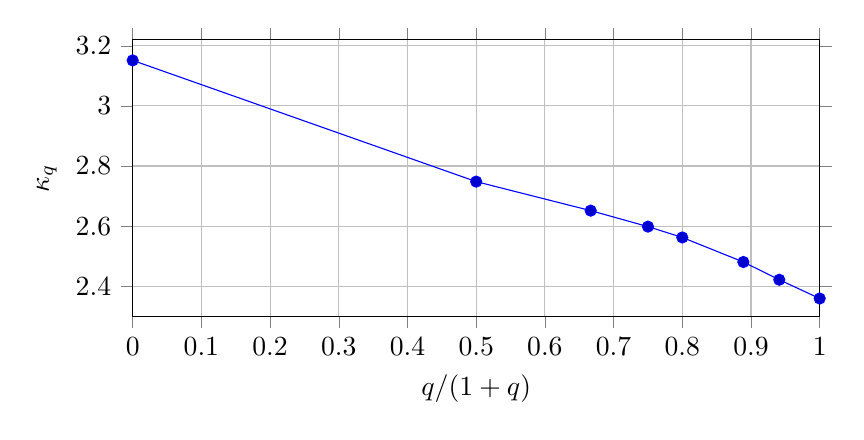
\begin{tikzpicture}
\begin{axis}[
 width=0.85\textwidth,
 height=0.42\textwidth,
 xlabel={$q/(1+q)$},
 ylabel={$\kappa_q$},
 xmin=0,xmax=1,
 ymin=2.30,ymax=3.22,
 grid=major,
 tick align=outside,
]
\addplot+[mark=*] coordinates {
 (0,3.1514961295)
 (0.5,2.7480700149)
 (0.6666666667,2.6514961295)
 (0.75,2.5983138062)
 (0.8,2.5622414703)
 (0.8888888889,2.4805809434)
 (0.9411764706,2.4214870020)
 (1,2.3590148791)
};
\end{axis}
\end{tikzpicture}
\end{center}

The monotone curve is not a cosmetic refinement: choosing one row answers one specific
notion of ``amplitude.''  Moving from $q=0$ to $q=\infty$ changes the power of $x$ by almost
$0.8$, an effect much larger than any logarithmic correction.

\section{Source-by-source reconciliation and correction of the draft}
\label{sec:source-reconciliation}

The pre-consolidation directory contained the original question, eight research reports, a
gentle guide, two audits, and two script suites.  Repetition was useful while the reports
were independent; it is harmful in the final account because later corrections can leave an
earlier theorem looking authoritative.  This section records exactly what was retained,
corrected, demoted, or generalized.  The complete pre-consolidation evidence remains
available in Git at commit
\texttt{2e3567feb14947ee3ebcdab11adca64e746ad26f}.

\subsection{Evidence-status legend}

Six statuses are kept separate throughout this volume.

\begin{enumerate}
\item \emph{Exact proof}: a complete argument is given here; many such results also have a
      named Lean declaration.
\item \emph{Imported theorem}: the product-specific reduction is proved here, while a
      precisely stated classical theorem such as RPF, a martingale limit theorem, or
      Carleman--Hoischen approximation is cited.
\item \emph{Rigorous certificate}: exact rational or interval arithmetic proves a stated
      enclosure, but does not validate every digit of a longer computed decimal.
\item \emph{Numerical evidence}: stable computation or collocation supports a value or
      pattern, but supplies neither interval certification nor a proof of a limit.
\item \emph{Frontier / conjectural}: a conjecture, proof architecture, or proposed
      strengthening is recorded with its missing bound or bridge stated explicitly.
\item \emph{Lean-source-only}: current Lean source contains an exact declaration, but this
      volume has not yet supplied the corresponding conventional proof.  Source presence
      and a fresh successful Lean build are reported separately.
\end{enumerate}

In particular, a long stable decimal is not a rigorous enclosure, an exhibited eigenvalue
is not automatically the second eigenvalue, and a formal Lean skeleton with an analytic
hypothesis is not a proof of that hypothesis.

\subsection{Source concordance}

\begin{center}
\small
\begin{tabularx}{\textwidth}{@{}>{\raggedright\arraybackslash}p{0.17\textwidth}
 X>{\raggedright\arraybackslash}p{0.29\textwidth}@{}}
\toprule
Source & Material retained & Adjudication in this volume\\
\midrule
Original 2018 question \cite{decay-draft}
 & Q2/Q3, finite Thue--Morse product-to-sum idea, reciprocal-Gamma and Pochhammer approach.
 & Questions restated precisely; formula (10) corrected in
   \Cref{thm:pochhammer-tail}; false radius inference removed.\\[0.35em]
Report 1 \cite{wave1-doc1}
 & Exact shell law, fixed rays, typical law, correct variance/CLT/LIL, integer-ratio
   generalization.
 & Dyadic core retained; integer-ratio result strengthened to
   \Cref{prop:global-spectral-pochhammer,thm:b-adic-variance}.\\[0.35em]
Report 2 \cite{wave1-doc2}
 & Calibrated Gelfond inequality, dense preimages, Lambert boundary layer, odd-multiple
   valleys.
 & Detailed extremal proofs retained in
   \Cref{sec:uniform,sec:annular-maxima,thm:odd-multiple-valley}.\\[0.35em]
Report 3 \cite{wave1-doc3}
 & First arithmetic-mean gauge and finite-$q$ spectrum.
 & Mean theory retained conditional on RPF; inherited LIL constant $\pi$ corrected to
   $\pi/\sqrt2$.\\[0.35em]
Report 4 \cite{wave1-doc4}
 & Systematic transfer operator, exact $q=0,2$ rows, rational $\rho_1$ certificate,
   fixed-offset valleys.
 & Retained; its continuum of intermediate rates remains explicitly conditional.\\[0.35em]
Reports 5--6 \cite{wave1-doc5,wave1-doc6}
 & Broad reconciliations, clean Gordin proof, numerical spectrum, source audit.
 & Deduplicated into the main spine; their \emph{adaptive gauge still open} status is
   superseded.\\[0.35em]
Report 7 \cite{wave1-doc7}
 & Bounded-distortion obstruction and first shell-adaptive analytic gauge.
 & Strong obstruction restored; malformed CLT quantifier corrected; smoothing replaced by
   the stronger Report 8 lemma.\\[0.35em]
Report 8 \cite{wave1-doc8}
 & Clean reciprocal construction, derivative-controlled flattening, analytic upgrade.
 & Canonical adaptive proof in \Cref{sec:adaptive-gauge}.\\[0.35em]
Comparative audit \cite{comparative-audit}
 & LIL forensic audit, grid and energy identities, peak--area comparison, RMS
   eigen-identities.
 & Exact pieces proved in \Cref{lem:peak-integral,prop:grid-identities,prop:L2-eigen-identities,prop:total-energy}; spectral-rate and peak-CLT overclaims
   demoted.\\[0.35em]
Second-wave audit \cite{second-wave-audit}
 & Corrected Q2 map, adversarial check of Reports 5--8, high-precision scripts.
 & Central logical corrections retained; its own appendix misprints are corrected below.\\[0.35em]
Gentle guide \cite{gentle-guide}
 & Accessible explanation of the log-square term, binary dynamics, four decay notions.
 & Intuition integrated into the introduction and proof commentary; unsupported numerical
   and \emph{formula-like gauge} language removed.\\
\bottomrule
\end{tabularx}
\end{center}

\subsection{Immutable source snapshot ledger}

The twelve absorbed TeX sources remain available at pre-consolidation commit
\nolinkurl{2e3567feb14947ee3ebcdab11adca64e746ad26f}.  To identify the precise inputs
independently of their filenames, the following are SHA-256 digests of the TeX bytes
extracted from that commit.

\begin{longtable}{@{}>{\raggedright\arraybackslash}p{0.24\textwidth}
 >{\raggedright\arraybackslash\ttfamily\scriptsize}p{0.70\textwidth}@{}}
\toprule
\normalfont\small Source & \normalfont\small SHA-256 of absorbed TeX\\
\midrule
\endhead
Original question & \nolinkurl{62586a1f0e6d9a12a23bfd38c006365ffc0bf897e84c6b4d3d318ac6c0c29b62}\\
Report 1 & \nolinkurl{27a9fda6220d3e3cde110919c40f1946ccdeff1463e8ef7a5055fbb6c26ef7ed}\\
Report 2 & \nolinkurl{df24e59e68f1cacf0aa1c26f1f48b0e6bb2a643fccf8ac805a96b373a56576a8}\\
Report 3 & \nolinkurl{ae5ba2d44c565ce826471893cf867d6cf4c365a0a5f580fdd4548d0a2dedb73d}\\
Report 4 & \nolinkurl{b0a76b35fbb9a9af78c469f07d94eb4346bfaeace20cca193b3c9afa97ed6816}\\
Report 5 & \nolinkurl{12af56c41c2a2dad549bddf77477e17ec47cf7a5d2dc65df1ca96dd89880b455}\\
Report 6 & \nolinkurl{de912bde5096ff4e4db8b4ad3a176e3f7c35551688fcf4bb450437626619a924}\\
Report 7 & \nolinkurl{17426ff49f76d580c922045d693fb215552a51e68e5a45cff8442d5a46cf9ad9}\\
Report 8 & \nolinkurl{a1dcad9e686f4f0b39ef326c953501a3e03eef7fbd9b8c05351bbaaa6c211749}\\
Comparative audit & \nolinkurl{871c3790ace2ce71bb906d17e96129aec79fcbb4fd069c412109b5da138e2ce7}\\
Second-wave audit & \nolinkurl{e2aa812e12ba613cdb89a7bce56814aa034db99b4db68457e46848340f480684}\\
Gentle guide & \nolinkurl{300cff33d98720436d655000b6d1070d1a86016e0ecc97235bc9e4b0a11f1791}\\
\bottomrule
\end{longtable}

\subsection{Why apparently different decay rates coexist}

The power of $x$ is determined by the numerator scale being sampled:
\[
 \frac12\quad(q=0),\qquad
 \rho_1\quad(q=1),\qquad
 \frac1{\sqrt2}\quad(q=2),\qquad
 \frac{\sqrt3}{2}\quad(q=\infty).
\]
Substitution into
$\kappa=\tfrac12+\log_2(\pi/\Lambda)$ gives four different, simultaneously correct
answers.  The old draft's value $\log_2(2\pi)$ is exactly the $q=2$ row.

The Lambert term is not a fifth power.  It refines the $q=\infty$ scale when comparison is
anchored at the left endpoint of a moving dyadic annulus.  The exact $4/3$ ray is sharp
relative to $E_{\kappa_\infty}$ at its own argument; the annular maximizer exploits the much
larger deterministic baseline nearer the left endpoint.  The fixed-offset and odd-multiple
valleys are different again: they describe exceptional individual lobes and force zero
liminf on the global-envelope scale.

\subsection{Correction ledger}

\begin{enumerate}
\item The published and Report 3 LIL constant $\pi$ with denominator
      $\sqrt{n\log\log n}$ is too large by $\sqrt2$.  The exact variance and Gordin
      decomposition prove $\pi/\sqrt2$; see \Cref{thm:exact-variance,thm:correct-lil}.
\item The original Pochhammer formula needs a negative exponent, denominator
      $1-4^{-k}$ independent of $m$, a sum beginning at $k=1$, and consistent prefix
      indices.  A convergence radius never implies that the represented entire function
      vanishes outside it.
\item The natural-gauge obstruction is not an impossibility theorem for all analytic or all
      elementary functions.  It excludes stabilizing and bounded-distortion shell shapes.
      The analytic adaptive gauge in \Cref{thm:analytic-adaptive} proves unrestricted Q2
      affirmatively.
\item The implication \emph{Hardy-field, hence elementary} is invalid.  Elementary
      oscillatory compositions can leave every Hardy field; the bounded oscillatory example
      before \Cref{sec:adaptive-gauge} is handled instead by bounded distortion.
\item The Gelfond estimate is sharp in exponential rate.  The lower orbit attains
      $(\sqrt3/2)^n$; the convenient upper bound with one fewer power is not itself attained
      for every $n$.
\item The eigen-identities at $-1/4$ are exact, but the \emph{second eigenvalue} claim and
      the $(-1/2)^n$ relative RMS rate were inferred from collocation.  They are not theorem
      statements here.
\item The limiting arithmetic profile is continuous and driven by the distribution function
      of an atomless singular measure.  Division by the mantissa contributes an ordinary
      absolutely continuous factor, so the profile itself is not a singular distribution
      function or a measure.
\item Complete logarithmic shells have masses converging to one common limit; they are not
      exactly equal at finite level.
\item Finite-grid profile calculations suggest excursions at least as far as roughly
      $0.91627$ and $1.11814$, but no interval-arithmetic argument certifies the global
      extrema of the limiting profile.
\item The comparative audit's peak CLT and limiting peak/area ratio require a certified
      cell-to-maximum transfer.  The rigorous peak--area inequality is retained, but the
      limit $1.92372\ldots$ remains numerical evidence.
\end{enumerate}

\subsection{Correct constants and their status}

The exact closed forms give
\[
 \begin{aligned}
 \kappa_0&=3.151496129472318798043279\ldots,\\
 \kappa_2&=2.651496129472318798043279\ldots,\\
 \kappa_\infty&=2.359014879111740707316409\ldots.
 \end{aligned}
\]
High-precision collocation, stable to substantially more digits than displayed but not an
interval proof, gives
\[
 \begin{aligned}
 \rho_1&=0.66132260206056561507352912\ldots,\\
 \kappa_1&=2.74807001487133267391714356\ldots,\\
 A_1&=0.09126612413158821228656307\ldots,\\
 B_1&=0.06505923504037692143099053\ldots,\\
 A_1^{\log}&=0.09386063575678126354068341\ldots.
 \end{aligned}
\]
The rigorous enclosures remain the much wider published and exact-rational intervals in
\Cref{prop:rho1-rigorous-bound}.  In particular, the longer decimals must not be cited as
certified.

The second-wave appendix itself had four unnoticed transcription errors: the tails of
$\kappa_0,\kappa_2,\kappa_\infty$ were printed incorrectly, and
$\rho_8$ was printed as $0.161244458899776$.  Its own bundled spectral data instead stabilize
at
\[
 \rho_8=0.1612444588997785467769607\ldots.
\]

\subsection{The literal Cesaro question, finally}

The natural gauge
\[
 g_1(x)=A_1x^{-\kappa_1}
 \exp\!\left(-\frac{(\log x)^2}{2\log2}\right)
\]
is positive, analytic, eventually decreasing, and has alternating derivative signs
eventually for each fixed derivative order.  It solves Q3, and Q2 along dyadic endpoints.
For unrestricted endpoints it has the nonconstant profile
\eqref{eq:phase-limit}.  No bounded-distortion shell correction can flatten that profile.
The shell-adaptive gauge $g_{\mathrm{ad}}$ escapes precisely by developing unbounded,
finer-and-finer microstructure and solves the literal unrestricted Q2.  If one insists on a
fixed nonadaptive scale, the logarithmic mean in \Cref{thm:logarithmic-mean} is the canonical
all-endpoint repair.

\subsection{Imported inputs and formalization boundary}

The product algebra, zero divisor, Thue--Morse sign, exact factorization, finite variance,
finite-grid Parseval, Gelfond inequality, Lambert optimization, peak--area estimate, and both
valley theorems are proved here.  The exact $L^2$ numerator identity and exponent are finite
Fourier algebra; convergence of the weighted shell-limit constant still uses RPF.  Four
classical analytic, ergodic, and probabilistic packages remain imported with their hypotheses
visible:

\begin{enumerate}
\item Ruelle--Perron--Frobenius quasi-compactness and simplicity for
      \eqref{eq:transfer-operator};
\item Birkhoff's ergodic theorem for the doubling and integer-base maps;
\item the distributional martingale CLT and the stationary reverse-martingale ASIP/LIL;
\item Carleman--Hoischen simultaneous approximation of a $C^1$ function and its derivative.
\end{enumerate}

The Collatz--Wielandt/Sturm appendix gives an exact machine-checkable enclosure for
$\rho_1$.  The verification scripts supply reproducible numerical evidence for the longer
constants and finite-level profiles, but they do not change that evidence category.  The
Lean cross-reference in \Cref{app:lean-crosswalk} records, theorem by theorem, which exact
substrate is already represented by exact Lean declarations and which analytic bridge remains a frontier.

\section{Conclusion}
\label{sec:conclusion}

The Fourier image of Rvachev's up-function has one deterministic core and several genuinely
different stochastic or extremal refinements.  The exact identity
\[
 |\FourierTwoPi{\RvachevUp}(2^ny)|
 =|\FourierTwoPi{\RvachevUp}(y)|\pi^{-n}y^{-n}2^{-n(n+1)/2}
 \prod_{j=1}^n|\sin(\pi2^jy)|
\]
separates them perfectly.  The triangular denominator produces
$-(\log x)^2/(2\log2)$.  The lacunary numerator then selects a pressure level:
Lebesgue geometric mean, Perron $L^1$ mean, Parseval $L^2$ mean, or maximizing orbit.

The final quantitative dictionary is:
\begin{align*}
 \kappa_0&=3.1514961294723187980\ldots &&\text{typical / geometric mean},\\
 \kappa_1&=2.7480700148713326739\ldots &&\text{arithmetic mean and Cesaro gauge},\\
 \kappa_2&=2.6514961294723187980\ldots &&\text{RMS; the old draft's exponent},\\
 \kappa_\infty&=2.3590148791117407073\ldots &&\text{sharp pointwise upper envelope}.
\end{align*}
The other three rows have exact closed forms; the displayed $\kappa_1$ digits are spectral
computation accompanied by a separate rigorous enclosure.
Typical logarithms fluctuate as
$(\pi/\sqrt2+\LittleO(1))\sqrt{(\log x/\log2)\log\log\log x}$ along the LIL extremal
subsequences.
Raw dyadic-annulus maxima carry an additional Lambert-$W$ term of order
$-(\log\log x)^2/(2\log2)$.  Fixed-offset lobe maxima after powers of two can instead have
the doubled leading coefficient $-(\log x)^2/\log2$.

For the question that originally motivated the investigation, the positive analytic gauge
$A_1E_{\kappa_1}$ gives the requested two-sided bounded Cesaro normalization and the exact
dyadic-endpoint limit.  Its failure at unrestricted endpoints, and the stronger
bounded-distortion obstruction, are structural: the last dyadic shell retains a singular
distribution of mass.  They do not contradict existence.  The adaptive gauge
$g_{\mathrm{ad}}$ develops the necessary finer-and-finer shell microstructure and solves the
literal unrestricted analytic problem.  Logarithmic averaging gives a simpler, fixed-scale
all-endpoint alternative.

The corrected Pochhammer theorem recovers the useful part of the original attempted answer
without confusing a local convergence disk with an asymptotic law.  Its arbitrary-radius
and integer-ratio extensions show that the dyadic case belongs to a broader family with
\[
 \kappa_{\mathrm{typ}}(b)=\frac12+\log_b(2\pi),
 \qquad
 \sigma_b^2=\frac{\pi^2}{12}\frac{b+1}{b-1}.
\]
Thus what looked like one irregular asymptotic is a compact pressure spectrum, one Lambert
boundary layer, several arithmetic valley mechanisms, and a clean geometric-ratio
universality class.  Every surviving claim now carries its proof status and source
provenance explicitly.

\appendix

\section{Exact Collatz--Wielandt certificate for \texorpdfstring{$\rho_1$}{rho1}}
\label{app:certificate}

The following SymPy script uses only exact rational arithmetic.  It constructs the rational
function in the proof of \Cref{prop:rho1-rigorous-bound}; Sturm's theorem, invoked by
\texttt{count\_roots}, certifies that the relevant numerators and denominators have no roots
on $[0,1]$.  Positivity at $t=0$ therefore proves positivity throughout the interval.

\begin{lstlisting}[style=code,language=Python]
import sympy as sp

t = sp.symbols("t", real=True)
u = 2*t/(1+t**2)
v = (1-t**2)/(1+t**2)

c = sp.Rational(376189, 10**6)
d = sp.Rational(-69093, 10**6)
e = sp.Rational(15483, 10**6)
p_cert = lambda z: 1 + c*z + d*z**2 + e*z**3

R = sp.cancel((u*p_cert(u) + v*p_cert(v)) / (2*p_cert(2*u*v)))
lo = sp.Rational(66126807, 10**8)
hi = sp.Rational(66134891, 10**8)

for expr in (R - lo, hi - R):
    num, den = map(lambda p: sp.Poly(p, t),
                   sp.together(expr).as_numer_denom())
    assert num.eval(0) > 0 and den.eval(0) > 0
    assert num.count_roots(0, 1) == 0
    assert den.count_roots(0, 1) == 0

print("Certified:", lo, "< rho_1 <", hi)
\end{lstlisting}

For the high-precision decimal, one may replace the exact certificate by a Chebyshev
collocation matrix.  The rapid stabilization displayed in \Cref{sec:numerics} is typical
for this analytic weighted-composition operator.

\section{Notation cross-reference}
\label{app:notation}

\begin{center}
\begin{tabularx}{\textwidth}{@{}lX@{}}
\toprule
Symbol & Meaning\\
\midrule
$\FourierTwoPi{\RvachevUp}$ & Fourier transform of Rvachev's up-function under the
$\EulerE^{-2\pi\ImaginaryUnit t\xi}$ convention\\
$a$ & $\log2$\\
$T$ & doubling map $x\mapsto2x\pmod1$\\
$s(x)$ & $\AbsoluteValue{\sin(\pi x)}$\\
$B_n(y)$ & $\prod_{j=1}^n s(T^jy)$\\
$E_\kappa(x)$ & $x^{-\kappa}\exp(- (\log x)^2/(2\log2))$\\
$W_\kappa(y)$ & bounded dyadic phase factor in \eqref{eq:master-normalization}\\
$\mathcal L_q$ & weighted Perron operator \eqref{eq:transfer-operator}\\
$\rho_q$ & Perron root of $\mathcal L_q$\\
$\Lambda_q$ & $\rho_q^{1/q}$, the $L^q$ numerator growth per dyadic level\\
$\kappa_q$ & sharp power in the normalized $L^q$ shell decay\\
$M_m$ & unique maximum of $\AbsoluteValue{\FourierTwoPi{\RvachevUp}}$ on $[m,m+1]$\\
\bottomrule
\end{tabularx}
\end{center}

\section{Lean declaration crosswalk and parity ledger}
\label{app:lean-crosswalk}

This appendix enforces the intended two-way documentation discipline.  It lists each
substantive theorem family used in this volume, not every implementation lemma.  An
\emph{exact} row means that current Lean source contains a theorem with the displayed
mathematical content; an \emph{abstract} row means Lean proves the deduction from explicit
hypotheses but not the analytic hypothesis itself.  The present document build does not by
itself constitute a fresh aggregate Lean compilation, so compilation evidence must be
reported separately from this source crosswalk.

\subsection{Human-readable results with exact Lean counterparts}

The middle column names declarations, not merely files.  All are in namespace
\lean{Fabius}.  Mixed results are split so a Lean declaration is never made to cover a
strictly stronger human theorem.

\begin{longtable}{@{}p{0.29\textwidth}p{0.40\textwidth}p{0.24\textwidth}@{}}
\toprule
Human-readable result & Exact Lean declaration(s) & Location in this volume\\
\midrule
\endfirsthead
\toprule
Human-readable result & Exact Lean declaration(s) & Location in this volume\\
\midrule
\endhead
Entire sinc product, evenness, real-axis reality, value at zero, and the classical
Fourier-product bridge
 & \decl{rvachevFourierProduct_differentiable},
   \decl{rvachevFourier_neg}, \decl{rvachevFourier_ofReal_im_eq_zero},
   \decl{rvachevFourier_zero}, \decl{rvachevFourier_eq_product}
 & \Cref{sec:introduction,sec:exact-products}\\
Super-polynomial real-axis decay of the Fourier transform
 & \decl{rvachevFourier_real_rapidDecay}
 & \Cref{cor:superpoly-subexp}\\
Energy from the dual-lattice samples, in two-sided form
\(\int\RvachevUp^2=\tfrac12\sum_{k\in\mathbb Z}\AbsoluteValue{\FourierTwoPi{\RvachevUp}(k/2)}^2\),
as an instance of interval Parseval for any time-limited square-integrable function
 & \decl{integral_sq_rvachevUp_eq_half_tsum_sq_rvachevFourier},
   \decl{integral_sq_rvachevUp_eq_half_add_tsum_sq_rvachevFourier},
   \decl{rvachevFourier_eq_fourierIntegral},
   \decl{IntervalParseval.integral_sq_eq_tsum_sq_fourierIntegral},
   \decl{IntervalParseval.integral_sq_eq_tsum_sq_fourierIntegral_of_le},
   \decl{IntSum.tsum_eq_zero_add_two_mul_tsum_odd}
 & \Cref{prop:total-energy} (second equality, in both its two-sided and its
   folded \(\tfrac12+\sum_{m\ge0}\) form; the decimal is not formal)\\
Exact nonzero complex zero set and analytic multiplicity $1+\TwoAdicValuation(m)$
 & \decl{rvachevFourierProduct_eq_zero_iff},
   \decl{analyticOrderAt_rvachevFourierProduct_int}
 & \Cref{prop:zero-divisor}\\
Exact zero-safe dyadic shell factorization and exponent algebra
 & \decl{norm_rvachevFourierProduct_two_pow_mul_cross},
   \decl{norm_rvachevFourierProduct_two_pow_mul},
   \decl{shell_exponent_identity}
 & \Cref{thm:exact-dyadic-factorization}\\
Finite Thue--Morse product-to-sum identity
 & \decl{prod_sin_two_pow_eq_thueMorse_sum}
 & \Cref{cor:finite-TM-sinc-expansion}\\
Strict central/side-lobe concavity, unique lobe maxima, and Thue--Morse lobe sign
 & \decl{strictConcaveOn_central_log_series},
   \decl{strictConcaveOn_lobe_log_series},
   \decl{existsUnique_isMaxOn_rvachevFourier_lobe},
   \decl{existsUnique_isMaxOn_rvachevFourier_neg_lobe},
   \decl{isMaxOn_norm_rvachevFourier},
   \decl{isMaxOn_rvachevFourier_central_eq_zero},
   \decl{rvachevFourier_eq_thueMorse_sign_mul_norm}
 & \Cref{thm:unique-extremum}\\
Sharp Gelfond inequality and equality orbit
 & \decl{abs_prod_sin_two_pow_le_sharp},
   \decl{abs_prod_sin_two_pow_third}
 & \Cref{prop:Bn-uniform}\\
Global envelope, exact fixed ray, and failure of every stronger exponent
 & \decl{norm_rvachevFourier_le_decayGauge},
   \decl{norm_rvachevFourier_peak_ray_envelope},
   \decl{not_exists_norm_rvachevFourierProduct_le_decayGauge_of_kappaInf_lt}
 & \Cref{thm:uniform-envelope,cor:universal-log-order}\\
Exact closed-form $\kappa_0,\kappa_2,\kappa_\infty$ dictionary, their ordering, and interval
certificates
 & \decl{kappaOf_half}, \decl{kappaOf_sqrt_two},
   \decl{kappaOf_sqrt_three}, \decl{kappaInf_lt_kappa_two},
   \decl{kappa_two_lt_kappa_zero}, \decl{kappa_zero_bracket},
   \decl{kappa_two_bracket}, \decl{kappa_inf_bracket}
 & \Cref{subsec:main-table,sec:uniform}\\
Continuous quadratic lacunary integral and dyadic-grid Parseval
 & \decl{integral_prod_sin_sq_two_pow},
   \decl{sum_prod_sin_sq_two_pow}
 & \Cref{eq:exact-L2-product,prop:grid-identities}\\
Root-of-unity sine product
 & \decl{prod_two_sin_pi_div_two_pow}
 & \Cref{prop:grid-identities}\\
Exact cocycle covariance, finite Birkhoff variance, and product bridge
 & \decl{integral_cocycle_covariance},
   \decl{integral_sq_birkhoff_sum_all},
   \decl{integral_sq_log_prod_two_sin_all}
 & \Cref{thm:exact-variance}\\
Gordin pointwise algebra and the $\pi^2/12,\pi^2/4$ Parseval values
 & \decl{two_log_two_sin_sub}, \decl{log_abs_tan_half_add},
   \decl{integral_sq_log_two_sin_pi_mul},
   \decl{integral_sq_log_abs_tan_pi_mul}
 & \Cref{sec:fluctuations}\\
One-step logarithmic centering identity underlying the geometric mean
 & \decl{integral_log_prod_two_sin}
 & \Cref{thm:geometric-mean}\\
Explicit $q=2$ transfer eigen-identities
 & \decl{rms_transfer_const_eigen}, \decl{rms_transfer_sin_eigen},
   \decl{rms_transfer_one_add_cos_eigen}
 & \Cref{prop:L2-eigen-identities}\\
Plancherel and sinc-square energy identities (not the half-integer sampling formula)
 & \decl{integral_norm_sq_rvachevFourier_eq_two_mul_fabiusSquareEnergy},
   \decl{fabiusSquareEnergy_eq_integral_Ioi_tprod_sinc_sq}
 & \Cref{prop:total-energy}\\
Global arbitrary-base spectral Pochhammer factorization
 & \decl{geometricSincProduct_eq_tprod_complexQPochhammerInf}
 & \Cref{prop:global-spectral-pochhammer}\\
Global dyadic Pochhammer and reciprocal-Gamma products (not the extracted tail series)
 & \decl{rvachevFourierProduct_eq_tprod_complexQPochhammerInf},
   \decl{dyadicReciprocalGamma_mul_neg},
   \decl{rvachevFourierProduct_eq_one_div_dyadicGamma_mul}
 & \Cref{thm:pochhammer-tail}\\
\bottomrule
\end{longtable}

\subsection[Lean-source-only proof debts]
{Exact Lean-source-only results still owed a conventional proof here}

These declarations are exact source statements, but the present volume uses them only as
context or supporting infrastructure and does not yet reproduce their full conventional
proofs.  They are therefore explicit documentation debts, not entries in the preceding
human-proof parity table.

\begin{longtable}{@{}p{0.34\textwidth}p{0.59\textwidth}@{}}
\toprule
Mathematical content & Exact Lean declaration(s)\\
\midrule
\endhead
Rapid real-axis decay of every positive-order iterated derivative
 & \decl{rvachevFourier_real_iteratedDeriv_rapidDecay}\\
Finite-level logarithmic concentration, an absolute-moment bound, and uniform
$\sqrt n$-scale tightness
 & \decl{measureReal_log_prod_ge_le}, \decl{tendsto_measureReal_log_prod_ge},
   \decl{measureReal_log_prod_sqrt_ge_le},
   \decl{integral_abs_log_prod_le}\\
Baseline $1/(\pi|x|)$ bound, global one-bound, and strictness away from zero
 & \decl{norm_rvachevFourier_le_inv}, \decl{norm_rvachevFourier_le_one},
   \decl{norm_rvachevFourier_lt_one_of_ne_zero},
   \decl{norm_rvachevFourier_eq_one_iff}\\
Existence and uniqueness of the transfer-supremum growth root (without its RPF spectral
identification)
 & \decl{exists_perron_exponent}, \decl{exists_perron_root},
   \decl{existsUnique_perron_root}\\
Lean Bernstein enclosures of that growth root and its $\kappa$ image
 & \decl{perron_bracket_pointwise}, \decl{perron_root_enclosure},
   \decl{kappa_one_enclosure}\\
\bottomrule
\end{longtable}

\subsection{Abstract Lean deductions whose analytic premises remain visible}

\begin{longtable}{@{}p{0.27\textwidth}p{0.32\textwidth}p{0.34\textwidth}@{}}
\toprule
Deduction formalized & Exact Lean declaration(s) & Missing product-specific input\\
\midrule
\endfirsthead
\toprule
Deduction formalized & Exact Lean declaration(s) & Missing product-specific input\\
\midrule
\endhead
Eventual two-sided Cesaro boundedness from normalized shell bounds
 & \decl{eventually_bounded_of_monotone_of_dyadic}
 & The $q=1$ RPF shell asymptotic\\
Dyadic profile aggregation from complete- and partial-shell limits
 & \decl{tendsto_cumulative_div_two_pow},
   \decl{tendsto_cumulative_profile}
 & Eigenmeasure convergence, atomlessness, and singularity\\
Logarithmic mean from convergent shell masses and bounded endpoint errors
 & \decl{tendsto_sum_add_bdd_div}
 & The concrete weighted shell limit\\
Partial-shell linearity forced by an unrestricted additive limit
 & \decl{tendsto_shell_increment}
 & The singular-measure contradiction for the sinc product\\
Finite-partition measure equalization and the diagonal selection mechanism
 & \decl{setIntegral_equalizer}, \decl{abs_setIntegral_equalizer_sub_le},
   \decl{exists_diagonal_tendsto_zero}
 & Smooth bridges, global gluing, and Carleman--Hoischen approximation\\
\bottomrule
\end{longtable}

\subsection{Human theorems still awaiting full Lean formalization}

The remaining frontier is now explicit rather than hidden in prose:

\begin{enumerate}
\item the full RPF eigenfunction/eigenmeasure/spectral-gap package for
      \eqref{eq:transfer-operator}, including the singular full-support $q=1$ eigenmeasure;
\item the resulting normalized finite-$q$ spectrum in \Cref{thm:Lq-spectrum} and the full
      $q=0$ geometric-mean and almost-everywhere typical-ray consequences, beyond the
      one-step centering integral and finite-level concentration already formalized;
\item the stationary martingale CLT and LIL applications, although their exact variance and
      coboundary algebra are formal;
\item the bounded-distortion obstruction and the completed smooth/analytic adaptive gauge;
\item the Lambert annular boundary layer and both complete peak-valley asymptotics, beyond
      the already formal local zero orders and global envelope;
\item the quantitative peak--area estimate and any eventual peak-height CLT;
\item the first-zero-extracted and arbitrary-$J$ Pochhammer series;
\item the strict human Collatz--Wielandt/Sturm bracket in
      \Cref{prop:rho1-rigorous-bound}; the existing Lean Bernstein certificate is a
      distinct, wider enclosure;
\item the integer-$b$ shell law, typical exponent, covariance, variance, and general
      martingale decomposition from \Cref{sec:integer-ratios};
\item nothing of \Cref{prop:total-energy} beyond its decimal: both equalities are
      formal (the Plancherel half in \lean{FabiusSquareEnergyFourier}, the half-integer
      sampling half in \lean{RvachevHalfIntegerEnergy}); the numerical value
      \(0.8088735\ldots\) remains computational evidence.
\end{enumerate}

The principal theorem families promoted in the prose now appear in the exact, abstract, or
unformalized ledger above, while exact Lean-source-only families are visibly recorded as
documentation debts.  Any future substantive Lean theorem added to the facade should add a
row here; any future theorem promoted in the prose should name its declaration or remain
visibly marked as imported, numerical, or frontier work.

\begin{thebibliography}{99}
\small

\bibitem{arias1982}
J. Arias de Reyna,
\emph{An infinitely differentiable function with compact support: Definition and properties},
English translation of \emph{Definici\'on y estudio de una funci\'on indefinidamente
diferenciable de soporte compacto}, Rev. Real Acad. Cienc. Exact. F\'is. Natur. Madrid
\textbf{76} (1982), 21--38; arXiv:1702.05442 (2017).

\bibitem{arias2018}
J. Arias de Reyna,
\emph{Arithmetic of the Fabius function},
Integers \textbf{18} (2018), Paper A51; arXiv:1702.06487.

\bibitem{baladi}
V. Baladi,
\emph{Positive Transfer Operators and Decay of Correlations},
Advanced Series in Nonlinear Dynamics, vol.~16, World Scientific, 2000.

\bibitem{fabius}
J. Fabius,
\emph{A probabilistic example of a nowhere analytic $C^\infty$-function},
Z. Wahrscheinlichkeitstheorie verw. Gebiete \textbf{5} (1966), 173--174,
\href{https://doi.org/10.1007/BF00536652}{doi:10.1007/BF00536652}.

\bibitem{fan1997}
A.-H. Fan,
\emph{Multifractal analysis of infinite products},
J. Statist. Phys. \textbf{86} (1997), 1313--1336,
\href{https://doi.org/10.1007/BF02183625}{doi:10.1007/BF02183625}.

\bibitem{fan-schmeling-shen}
A. Fan, J. Schmeling, and W. Shen,
\emph{$L^\infty$-estimation of generalized Thue--Morse trigonometric polynomials and
ergodic maximization},
Discrete Contin. Dyn. Syst. \textbf{41} (2021), 297--327,
\href{https://doi.org/10.3934/dcds.2020363}{doi:10.3934/dcds.2020363}.

\bibitem{gelfond}
A. O. Gel'fond,
\emph{Sur les nombres qui ont des propri\'et\'es additives et multiplicatives donn\'ees},
Acta Arith. \textbf{13} (1967/68), 259--265,
\href{https://doi.org/10.4064/aa-13-3-259-265}{doi:10.4064/aa-13-3-259-265}.

\bibitem{gauthier-kienzle}
P. M. Gauthier and J. Kienzle,
\emph{Approximation of a function and its derivatives by entire functions},
Canad. Math. Bull. \textbf{59} (2016), no.~1, 87--94,
\href{https://doi.org/10.4153/CMB-2015-060-5}{doi:10.4153/CMB-2015-060-5}.

\bibitem{corless-lambert}
R. M. Corless, G. H. Gonnet, D. E. G. Hare, D. J. Jeffrey, and D. E. Knuth,
\emph{On the Lambert $W$ function},
Adv. Comput. Math. \textbf{5} (1996), 329--359,
\href{https://doi.org/10.1007/BF02124750}{doi:10.1007/BF02124750}.

\bibitem{jessen-wintner}
B. Jessen and A. Wintner,
\emph{Distribution functions and the Riemann zeta function},
Trans. Amer. Math. Soc. \textbf{38} (1935), 48--88.

\bibitem{mse-extrema}
V. Reshetnikov,
\emph{Extrema of an infinite product of sinc functions},
Mathematics Stack Exchange, question 2742261 (2018),
\url{https://math.stackexchange.com/questions/2742261/}.

\bibitem{mse-decay}
V. Reshetnikov,
\emph{Asymptotic decay rate of an infinite product of sinc functions},
Mathematics Stack Exchange, question 2745497 (2018),
\url{https://math.stackexchange.com/questions/2745497/}.

\bibitem{proveit}
V. Reshetnikov,
\emph{ProveIt: Analysis/FabiusFunction}, GitHub repository,
\url{https://github.com/VladimirReshetnikov/ProveIt/tree/main/Analysis/FabiusFunction}.

\bibitem{decay-draft}
V. Reshetnikov,
\emph{Asymptotic decay rate of an infinite product of sinc functions}, source draft in the
\texttt{ProveIt} repository,
\url{https://github.com/VladimirReshetnikov/ProveIt/blob/2e3567feb14947ee3ebcdab11adca64e746ad26f/Analysis/FabiusFunction/docs/semi-formalized-research-frontiers/drafts/rvachev_up_fourier_decay/asymptotic-decay-rate-of-an-infinite-product-of-sinc-functions/asymptotic-decay-rate-of-an-infinite-product-of-sinc-functions.tex}.

\bibitem{queffelec}
M. Queff\'elec,
\emph{Questions around the Thue--Morse sequence},
Unif. Distrib. Theory \textbf{13} (2018), no.~1, 1--25,
\href{https://doi.org/10.1515/udt-2018-0001}{doi:10.1515/udt-2018-0001}.

\bibitem{rvachev1971}
V. L. Rvachev and V. A. Rvachev,
\emph{On one compactly supported function},
Dokl. Akad. Nauk Ukrainian SSR, Ser.~A, no.~8 (1971), 705--707
(in Ukrainian).


\bibitem{ahl2017}
C. Aistleitner, R. Hofer, and G. Larcher,
\emph{On evil Kronecker sequences and lacunary trigonometric products},
Ann. Inst. Fourier (Grenoble) \textbf{67} (2017), no.~2, 637--687,
\href{https://doi.org/10.5802/aif.3094}{doi:10.5802/aif.3094};
preprint arXiv:1502.06738.

\bibitem{fouvrymauduit1996}
\'E. Fouvry and C. Mauduit,
\emph{Sommes des chiffres et nombres presque premiers},
Math. Ann. \textbf{305} (1996), no.~3, 571--600,
\href{https://doi.org/10.1007/BF01444238}{doi:10.1007/BF01444238}.

\bibitem{cuny-merlevede2015}
C. Cuny and F. Merlev\`ede,
\emph{Strong invariance principles with rate for ``reverse'' martingale differences and
applications},
J. Theoret. Probab. \textbf{28} (2015), no.~1, 137--183,
\href{https://doi.org/10.1007/s10959-013-0506-z}{doi:10.1007/s10959-013-0506-z}.

\bibitem{wave1-doc1}
\emph{Rvachev up Fourier decay, Wave 1, Document 1}, working report in the
\texttt{ProveIt} repository,
\url{https://github.com/VladimirReshetnikov/ProveIt/blob/2e3567feb14947ee3ebcdab11adca64e746ad26f/Analysis/FabiusFunction/docs/semi-formalized-research-frontiers/drafts/rvachev_up_fourier_decay/rvachev_up_fourier_decay-1/rvachev_up_fourier_decay.tex}.

\bibitem{wave1-doc2}
\emph{Rvachev up Fourier decay, Wave 1, Document 2}, working report in the
\texttt{ProveIt} repository,
\url{https://github.com/VladimirReshetnikov/ProveIt/blob/2e3567feb14947ee3ebcdab11adca64e746ad26f/Analysis/FabiusFunction/docs/semi-formalized-research-frontiers/drafts/rvachev_up_fourier_decay/Rvachev_Up_Fourier_Decay-2/Rvachev_Up_Fourier_Decay.tex}.

\bibitem{wave1-doc3}
\emph{Fourier decay of Rvachev up, Wave 1, Document 3}, working report in the
\texttt{ProveIt} repository,
\url{https://github.com/VladimirReshetnikov/ProveIt/blob/2e3567feb14947ee3ebcdab11adca64e746ad26f/Analysis/FabiusFunction/docs/semi-formalized-research-frontiers/drafts/rvachev_up_fourier_decay/Rvachev_Up_Fourier_Decay-3/Fourier_decay_of_Rvachev_up.tex}.

\bibitem{wave1-doc4}
\emph{Rvachev up Fourier decay, Wave 1, Document 4}, working report in the
\texttt{ProveIt} repository,
\url{https://github.com/VladimirReshetnikov/ProveIt/blob/2e3567feb14947ee3ebcdab11adca64e746ad26f/Analysis/FabiusFunction/docs/semi-formalized-research-frontiers/drafts/rvachev_up_fourier_decay/rvachev_up_fourier_decay-4/rvachev_up_fourier_decay.tex}.

\bibitem{wave1-doc5}
\emph{Rvachev up Fourier decay, Report 5}, working report in the
\texttt{ProveIt} repository,
\url{https://github.com/VladimirReshetnikov/ProveIt/blob/2e3567feb14947ee3ebcdab11adca64e746ad26f/Analysis/FabiusFunction/docs/semi-formalized-research-frontiers/drafts/rvachev_up_fourier_decay/rvachev_up_fourier_decay-5/Rvachev_Up_Fourier_Decay_Final.tex}.

\bibitem{wave1-doc6}
\emph{Rvachev up Fourier decay, Report 6 final synthesis}, working report in the
\texttt{ProveIt} repository,
\url{https://github.com/VladimirReshetnikov/ProveIt/blob/2e3567feb14947ee3ebcdab11adca64e746ad26f/Analysis/FabiusFunction/docs/semi-formalized-research-frontiers/drafts/rvachev_up_fourier_decay/rvachev_up_fourier_decay-6/Rvachev_Up_Fourier_Decay_Final_Synthesis.tex}.

\bibitem{wave1-doc7}
\emph{Rvachev up Fourier decay, Report 7}, working report in the
\texttt{ProveIt} repository,
\url{https://github.com/VladimirReshetnikov/ProveIt/blob/2e3567feb14947ee3ebcdab11adca64e746ad26f/Analysis/FabiusFunction/docs/semi-formalized-research-frontiers/drafts/rvachev_up_fourier_decay/rvachev_up_fourier_decay-7/rvachev_up_fourier_decay_final.tex}.

\bibitem{wave1-doc8}
\emph{Rvachev up Fourier decay, Report 8}, working report in the
\texttt{ProveIt} repository,
\url{https://github.com/VladimirReshetnikov/ProveIt/blob/2e3567feb14947ee3ebcdab11adca64e746ad26f/Analysis/FabiusFunction/docs/semi-formalized-research-frontiers/drafts/rvachev_up_fourier_decay/rvachev_up_fourier_decay-8/rvachev_up_fourier_decay_final.tex}.

\bibitem{comparative-audit}
\emph{Rvachev up Fourier decay comparative audit}, working report in the
\texttt{ProveIt} repository,
\url{https://github.com/VladimirReshetnikov/ProveIt/blob/2e3567feb14947ee3ebcdab11adca64e746ad26f/Analysis/FabiusFunction/docs/semi-formalized-research-frontiers/drafts/rvachev_up_fourier_decay/Rvachev_Up_Fourier_Decay_Comparative_Audit/Rvachev_Up_Fourier_Decay_Comparative_Audit.tex}.

\bibitem{second-wave-audit}
\emph{Rvachev up Fourier decay second-wave audit}, working report in the
\texttt{ProveIt} repository,
\url{https://github.com/VladimirReshetnikov/ProveIt/blob/2e3567feb14947ee3ebcdab11adca64e746ad26f/Analysis/FabiusFunction/docs/semi-formalized-research-frontiers/drafts/rvachev_up_fourier_decay/Rvachev_Up_Fourier_Decay_Second_Wave_Audit/Rvachev_Up_Fourier_Decay_Second_Wave_Audit.tex}.

\bibitem{gentle-guide}
\emph{Rvachev up Fourier decay: a gentle guide}, working report in the
\texttt{ProveIt} repository,
\url{https://github.com/VladimirReshetnikov/ProveIt/blob/2e3567feb14947ee3ebcdab11adca64e746ad26f/Analysis/FabiusFunction/docs/semi-formalized-research-frontiers/drafts/rvachev_up_fourier_decay/Rvachev_Up_Fourier_Decay_Gentle_Guide/Rvachev_Up_Fourier_Decay_Gentle_Guide.tex}.

\end{thebibliography}

\end{document}
